%%%%%%%%%%%%%%%%%%%%%%%%%%%%%%%%%%%%%%%%%%%%%%%%%%%%%%%%%%%%%%%%%%
%%%%%%%%%%%%%%%%%%%%%%%%%%%%%%%%%%%%%%%%%%%%%%%%%%%%%%%%%%%%%%%%%%
\chapter{Klassische nonparametrische Methoden}
\label{sec:bioStat}
%%%%%%%%%%%%%%%%%%%%%%%%%%%%%%%%%%%%%%%%%%%%%%%%%%%%%%%%%%%%%%%%%%
%%%%%%%%%%%%%%%%%%%%%%%%%%%%%%%%%%%%%%%%%%%%%%%%%%%%%%%%%%%%%%%%%%

\index{nonparametrische Methoden}
\index{verteilungsfreie Methoden|see{nonparametrische Methoden}}
Wenn inferenzstatistische Tests zur Datenauswertung herangezogen werden sollen, aber davon ausgegangen werden muss, dass strenge Anforderungen an die Art und Qualität der erhobenen Daten nicht erfüllt sind, kommen viele konventionelle Verfahren womöglich nicht in Betracht. 
Dagegen haben nonparametrische Methoden weniger restriktive Voraussetzungen und kommen auch bei kleinen Stichproben in Frage \cite{Bortz2008a, Buning1994}. Auch für (gemeinsame) Häufigkeiten kategorialer Variablen sowie ordinale Daten\footnote{Auf Rangdaten basierende Tests machen häufig die Voraussetzung, dass die Ränge eindeutig bestimmbar sind, also keine gleichen Werte (\emph{Bindungen}, \emph{ties}) auftauchen. Für den Fall, dass dennoch Bindungen vorhanden sind, existieren unterschiedliche Strategien, wobei die von R-Funktionen gewählte häufig in der zugehörigen Hilfe erwähnt wird.} sind viele der folgenden Methoden geeignet und ergänzen damit die in Kap.\ \ref{sec:glm} vorgestellten Modelle.

Einige der klassischen nonparametrischen Methoden approximieren die unbekannte oder nicht praktisch berechenbare Verteilung der verwendeten Teststatistik durch eine mit wachsender Stichprobengröße asymptotisch gültige Verteilung, die analytisch bestimmbar ist. Einen anderen Weg gehen die in Kap.\ \ref{sec:resampling} vorgestellten Resampling-Verfahren (bootstrap und Permutationstests), die die Verteilung der Teststatistik allein auf Basis der gezogenen Stichprobe und vieler zufälliger neuer Versionen von ihr schätzen.

%%%%%%%%%%%%%%%%%%%%%%%%%%%%%%%%%%%%%%%%%%%%%%%%%%%%%%%%%%%%%%%%%%
%%%%%%%%%%%%%%%%%%%%%%%%%%%%%%%%%%%%%%%%%%%%%%%%%%%%%%%%%%%%%%%%%%
\section{Anpassungstests}
\label{sec:modelTests}
%%%%%%%%%%%%%%%%%%%%%%%%%%%%%%%%%%%%%%%%%%%%%%%%%%%%%%%%%%%%%%%%%%
%%%%%%%%%%%%%%%%%%%%%%%%%%%%%%%%%%%%%%%%%%%%%%%%%%%%%%%%%%%%%%%%%%

Viele Tests setzen voraus, dass die Verteilung der Zielgröße in den untersuchten Bedingungen bekannt ist und bestimmte Voraussetzungen erfüllt -- oft muss es sich etwa um eine Normalverteilung handeln. Ob die erhobenen Werte in einer bestimmten Stichprobe mit einer solchen Annahme verträglich sind, kann mit verschiedenen Anpassungstests geprüft werden.

Solche \emph{goodness-of-fit} Tests werden meist mit der $\text{H}_{0}$ durchgeführt, dass eine bestimmte Verteilung vorliegt und dieses Vorliegen auch den gewünschten Zustand beschreibt. Da hier die $\text{H}_{1}$ gegen die fälschliche Nicht-Annahme abzusichern ist, muss der $\beta$-Fehler kontrolliert, also eine gewisse power gesichert werden. Mitunter wird dafür das $\alpha$-Niveau höher als üblich gewählt (in der Größenordnung von $0.2$), auch wenn sich der $\beta$-Fehler so nicht exakt begrenzen lässt. Angemessenere Herangehensweisen beschreibt \citeA{Wellek2010}.

%%%%%%%%%%%%%%%%%%%%%%%%%%%%%%%%%%%%%%%%%%%%%%%%%%%%%%%%%%%%%%%%%%
%%%%%%%%%%%%%%%%%%%%%%%%%%%%%%%%%%%%%%%%%%%%%%%%%%%%%%%%%%%%%%%%%%
\subsection{Binomialtest}
\label{sec:binomTest}
%%%%%%%%%%%%%%%%%%%%%%%%%%%%%%%%%%%%%%%%%%%%%%%%%%%%%%%%%%%%%%%%%%
%%%%%%%%%%%%%%%%%%%%%%%%%%%%%%%%%%%%%%%%%%%%%%%%%%%%%%%%%%%%%%%%%%

\index{Binomialtest}
Der Binomialtest ist auf Daten von Variablen anzuwenden, die nur zwei Ausprägungen annehmen können. Eine Ausprägung soll dabei als \emph{Treffer} bzw.\ \emph{Erfolg} bezeichnet werden. Der Test prüft, ob die empirische Auftretenshäufigkeit eines Treffers in einer Stichprobe verträglich mit der $\text{H}_{0}$ einer bestimmten\index[func]{binom.test()@\lstinline{binom.test()}} Trefferwahrscheinlichkeit $p_{0}$ ist.
\begin{lstlisting}
binom.test(x=<<Erfolge>>, n=<<Stichprobengröße>>, p=0.5, conf.level=0.95,
           alternative=c("two.sided", "less", "greater"))
\end{lstlisting}

Unter \lstinline!x! ist die beobachtete Anzahl der Erfolge anzugeben, \lstinline!n! steht für die Stichprobengröße. Alternativ zur Angabe von \lstinline!x! und \lstinline!n! kann als erstes Argument ein Vektor mit zwei Elementen übergeben werden, dessen Einträge die Anzahl der Erfolge und Misserfolge sind -- etwa das Ergebnis einer Häufigkeitsauszählung mit \lstinline!xtabs()!. Unter \lstinline!p! ist $p_{0}$ einzutragen. Das Argument \lstinline!alternative! bestimmt, ob zweiseitig (\lstinline!"two.sided"!), links- (\lstinline!"less"!) oder rechtsseitig (\lstinline!"greater"!) getestet wird. Die Aussage bezieht sich dabei auf die Reihenfolge $p_{1}$ \lstinline!"less"! bzw.\ \lstinline!"greater"! $p_{0}$, mit $p_{1}$ als Trefferwahrscheinlichkeit unter $\text{H}_{1}$. Mit dem Argument \lstinline!conf.level! wird die Breite des Konfidenzintervalls für $p$ festgelegt.\footnote{Das Intervall ist jenes nach Clopper-Pearson. Für die Berechnung u.\,a.\ nach Wilson, Agresti-Coull und Jeffreys vgl.\ \lstinline!BinomCI()!\index[func]{BinomCI()@\lstinline{BinomCI()}} aus dem\index[pack]{DescTools@\lstinline{DescTools}} Paket \lstinline!DescTools!.}

Als Beispiel sollen aus einer (unendlich großen) Urne zufällig Lose gezogen werden, wobei $p_{0} = 0.25$ ist. Es sei nach der Wahrscheinlichkeit gefragt, bei mindestens $5$ von insgesamt $7$ Ziehungen einen Gewinn zu ziehen.
\begin{lstlisting}
> draws <- 7                       # Stichprobenumfang
> hits  <- 5                       # Anzahl Treffer
> pH0   <- 0.25                    # Trefferwahrscheinlichkeit unter H0
> binom.test(hits, draws, p=pH0, alternative="greater", conf.level=0.95)
Exact binomial test
data: hits and draws
number of successes = 5, number of trials = 7, p-value = 0.01288
alternative hypothesis: true probability of success is greater than 0.25
95 percent confidence interval:
0.3412614 1.0000000
sample estimates:
probability of success
0.7142857
\end{lstlisting}

Das Ergebnis enthält neben einer Zusammenfassung der eingegebenen Daten (\lstinline!number of successes! und \lstinline!number of trials!, \lstinline!probability of success!) den $p$-Wert (\lstinline!p-value!). Schließlich wird je nach Fragestellung das zwei-, links- oder rechtsseitige Konfidenzintervall für die Trefferwahrscheinlichkeit in der gewünschten Breite genannt. Der ausgegebene $p$-Wert kann manuell mit Hilfe der Verteilungsfunktion der Binomialverteilung verifiziert werden (Abschn.\ \ref{sec:distrFunc}, Fußnote \ref{ftn:distrFuncDiscr}).
\begin{lstlisting}
> (pVal <- pbinom(hits-1, draws, pH0, lower.tail=FALSE))
[1] 0.01287842
\end{lstlisting}

Für den zweiseitigen Binomialtest existieren verschiedene Definitionen des $p$-Wertes als Wahrscheinlichkeit unter $\text{H}_{0}$, mindestens so extreme Trefferzahlen wie die beobachtete zu erhalten:
\begin{enumerate}
\item R summiert die Wahrscheinlichkeiten unter Gültigkeit der $\text{H}_{0}$ für alle Ereignisse mit höchstens der Wahrscheinlichkeit des eingetretenen Ereignisses. So ist etwa der von \lstinline!binom.test(10, 20, p=0.25, alternative="two.sided")! ausgegebene $p$-Wert gleich \lstinline!sum(dbinom(10:20, 20, 0.25)) + sum(dbinom(0, 20, 0.25))!. Die {\quotedblbase}Extremheit{\textquotedblleft} eines Ereignisses wird hier also i.\,S.\ seiner Wahrscheinlichkeit verstanden.
\item Zwei andere Definition beziehen sich auf die separaten einseitigen Tests: Für sie muss im Beispiel zum einen die Wahrscheinlichkeit von $5$ oder mehr Gewinnen unter $\text{H}_{0}$ berechnet werden, zum anderen die Wahrscheinlichkeit von $2$ (also $7-5$) Treffern oder weniger. Der zweiseitige $p$-Wert kann nun als das Doppelte des kleineren der $p$-Werte der einseitigen Tests definiert werden.
\item Als weitere Möglichkeit können die $p$-Werte für jede der beiden einseitigen Fragestellungen addiert werden.
\end{enumerate}

Wenn unter $\text{H}_{0}$ mit $p=0.5$ eine symmetrische Binomialverteilung vorliegt, führen die genannten Definitionen zum selben Ergebnis. Nach einer gängigen Konvention ist beim zweiseitigen Test auf jeder Seite $\frac{\alpha}{2}$ einzuhalten, auch wenn bei Überschreitung von $\frac{\alpha}{2}$ auf einer Seite dennoch insgesamt $p < \alpha$ wäre.
\begin{lstlisting}
# rechtsseitiger Test
> resG <- binom.test(hits, draws, p=pH0, alternative="greater")
> resG$p.value                                      # p-Wert
[1] 0.01287842

# linksseitiger Test
> resL <- binom.test(draws-hits, draws, p=pH0, alternative="less")
> resL$p.value                                      # p-Wert
[1] 0.7564087

# Gesamt-p-Werte
> 2 * min(c(resG$p.value, resL$p.value))            # Variante 2
[1] 0.02575684
\end{lstlisting}

Hypothesen über die jeweiligen Trefferwahrscheinlichkeiten einer dichotomen Variable in zwei unabhängigen Stichproben lassen sich mit Fishers exaktem Test prüfen (Abschn.\ \ref{sec:fisherEq}), in zwei abhängigen Stichproben mit dem McNemar-Test (Abschn.\ \ref{sec:mcNemar}), in mehr als zwei unabhängigen Stichproben mit einem $\chi^{2}$-Test (Abschn.\ \ref{sec:propTest}) und in mehr als zwei abhängigen Stichproben mit Cochrans $Q$-Test (Abschn.\ \ref{sec:cochranQ}).

%%%%%%%%%%%%%%%%%%%%%%%%%%%%%%%%%%%%%%%%%%%%%%%%%%%%%%%%%%%%%%%%%%
%%%%%%%%%%%%%%%%%%%%%%%%%%%%%%%%%%%%%%%%%%%%%%%%%%%%%%%%%%%%%%%%%%
\subsection{Test auf Zufälligkeit (Runs-Test)}
\label{sec:runsTest}
%%%%%%%%%%%%%%%%%%%%%%%%%%%%%%%%%%%%%%%%%%%%%%%%%%%%%%%%%%%%%%%%%%
%%%%%%%%%%%%%%%%%%%%%%%%%%%%%%%%%%%%%%%%%%%%%%%%%%%%%%%%%%%%%%%%%%

\index{Runs-Test}
\index{Iterationslängentest|see{Runs-Test}}
Eine zufällige Reihenfolge von $N$ Ausprägungen einer dichotomen Variable sollte sich dann ergeben, wenn die Erfolgswahrscheinlichkeit für jede Realisierung konstant $p$ beträgt und die Realisierungen unabhängig sind. Mit dem Test auf Zufälligkeit kann geprüft werden, ob eine empirische Datenreihe mit der Annahme von Zufälligkeit verträglich ist. Teststatistik $R$ ist die Anzahl der Iterationen (\emph{runs}, Abschn.\ \ref{sec:runs}), wobei sowohl eine sehr geringe als auch eine sehr hohe Anzahl gegen die $\text{H}_{0}$ spricht.

Eine spezielle Funktion für den Test auf Zufälligkeit ist nicht im Basisumfang von R enthalten,\footnote{Vergleiche hierfür \lstinline!RunsTest()!\index[func]{RunsTest()@\lstinline{RunsTest()}} aus dem\index[pack]{DescTools@\lstinline{DescTools}} \lstinline!DescTools! Paket.} eine manuelle Durchführung jedoch möglich. Als Beispiel diene jenes aus \citeA[p.~548~ff.]{Bortz2008a}: Bei einer Warteschlange aus $8$ Personen ($5$ Frauen, \lstinline!f! und $3$ Männer, \lstinline!m!) wird das Geschlecht des an jeder Position Wartenden erhoben.
\begin{lstlisting}
> queue <- c("f", "m", "m", "f", "m", "f", "f", "f")         # Daten
> Nj    <- xtabs(~ queue)                      # Gruppengrößen
> (runs <- rle(queue))                         # Iterationen
Run Length Encoding
lengths: int [1:5] 1 2 1 1 3
values: chr [1:5] "f" "m" "f" "m" "f"

> (rr <- length(runs$lengths))                 # Gesamtzahl Iterationen
[1] 5

> (rr1 <- xtabs(~ runs$values)[1])             # Iterationen Gruppe 1
f
3

> (rr2 <- xtabs(~ runs$values)[2])             # Iterationen Gruppe 2
m
2
\end{lstlisting}

Für den $p$-Wert des beobachteten Wertes von $R$ sind die Punktwahrscheinlichkeiten für alle Fälle aufzuaddieren, die dieses $R$ oder extremere Werte ergeben. Die Berechnung der Punktwahrscheinlichkeiten geschieht hier mit einer eigens erstellten Funktion (Abschn.\ \ref{sec:function}). Für die Ermittlung des $p$-Wertes ist zu beachten, dass ein ungerades $R$ generell auf zwei Arten zustande kommen kann: Entweder ist die Anzahl der Iterationen der ersten Gruppe um $1$ größer als die der zweiten, oder umgekehrt. Hier sind die Fälle für $R = 5, 6, 7$ zu berücksichtigen -- der Obergrenze möglicher Iterationen. Der Fall $R = 7$ kann sich hier nur auf eine Weise ergeben, da nur $3$ Männer vorhanden sind, so dass insgesamt $4$ Punktwahrscheinlichkeiten zu addieren sind.
\begin{lstlisting}
# Funktion, um Punktwahrscheinlichkeit für Anzahl von Iterationen der
# Gruppe 1 (r1), Gruppe 2 (r2), mit Gruppengrößen n1 & n2 zu berechnen
> getP <- function(r1, r2, n1, n2) {
+   # Punktwahrscheinlichkeit für r1+r2 ungerade
+   p <- (choose(n1-1, r1-1) * choose(n2-1, r2-1)) / choose(n1+n2, n1)
+
+   # Punktwahrscheinlichkeit für r1+r2 gerade: 2*ungerade
+   ifelse(((r1+r2) %% 2) == 0, 2*p, p)
+ }

> n1   <- Nj[1]                                  # Größe Gruppe 1
> n2   <- Nj[2]                                  # Größe Gruppe 2
> N    <- sum(Nj)                                # Gesamt-N
> rMin <- 2                # Untergrenze für Anzahl der Iterationen

# Obergrenze Anzahl Iterationen, Fallunterscheidung: n1 == n2?
> (rMax <- ifelse(n1 == n2, N, 2*min(c(n1, n2)) + 1))
[1] 7

# addiere Punktwahrscheinlichkeiten für R=beobachtet und größer
> p3.2   <- getP(3, 2, n1, n2)                   # r1=3, r2=2 -> R=5
> p2.3   <- getP(2, 3, n1, n2)                   # r1=2, r2=3 -> R=5
> p3.3   <- getP(3, 3, n1, n2)                   # r1=3, r2=3 -> R=6
> p4.3   <- getP(4, 3, n1, n2)                   # r1=4, r2=3 -> R=7
> (pGrEq <- p3.2 + p2.3 + p3.3 + p4.3)           # p-Wert einseitig
0.5714286

# Punktwahrscheinlichkeit aller anderen Fälle
> p2.2   <- getP(2, 2, n1, n2)                   # r1=2, r2=2 -> R=4
> p1.2   <- getP(1, 2, n1, n2)                   # r1=1, r2=2 -> R=3
> p2.1   <- getP(2, 1, n1, n2)                   # r1=2, r2=1 -> R=3
> p1.1   <- getP(1, 1, n1, n2)                   # r1=1, r2=1 -> R=2
> (pLess <- p2.2 + p1.2 + p2.1 + p1.1)
0.4285714

> pGrEq + pLess                     # Kontrolle: Summe beider Wkt. = 1
[1] 1
\end{lstlisting}

Aus $R$ lässt sich eine mit wachsender Stichprobengröße asymptotisch standardnormalverteilte Teststatistik berechnen, deren Verwendung ab einer Anzahl von ca.\ $30$ Beobachtungen nur zu geringen Fehlern führen sollte.
\begin{lstlisting}
> muR   <- 1 + ((2*n1*n2) / N)                   # Erwartungswert von R
> varR  <- (2*n1*n2*(2*n1*n2 - N)) / (N^2 * (N-1))      # Varianz von R
> rZ    <- (rr-muR) / sqrt(varR)                 # z-Transformiertes R
> (pVal <- pnorm(rZ, lower.tail=FALSE))          # p-Wert einseitig
0.4184066
\end{lstlisting}

\index{Wald-Wolfowitz-Test}
In Form des Wald-Wolfowitz-Tests lässt sich auch prüfen, ob zwei Stichproben aus derselben Grundgesamtheit stammen bzw.\ ob die zu ihnen gehörenden Variablen dieselbe Verteilung besitzen. Dazu werden die Daten beider Stichproben gemeinsam ihrer Größe nach geordnet. Anschließend ist jeder Wert durch die Angabe zu ersetzen, aus welcher Stichprobe er stammt und der Test wie jener auf Zufälligkeit durchzuführen.

%%%%%%%%%%%%%%%%%%%%%%%%%%%%%%%%%%%%%%%%%%%%%%%%%%%%%%%%%%%%%%%%%%
%%%%%%%%%%%%%%%%%%%%%%%%%%%%%%%%%%%%%%%%%%%%%%%%%%%%%%%%%%%%%%%%%%
\subsection{Kolmogorov-Smirnov-Anpassungstest}
\label{sec:ksTest}
%%%%%%%%%%%%%%%%%%%%%%%%%%%%%%%%%%%%%%%%%%%%%%%%%%%%%%%%%%%%%%%%%%
%%%%%%%%%%%%%%%%%%%%%%%%%%%%%%%%%%%%%%%%%%%%%%%%%%%%%%%%%%%%%%%%%%

\index{Kolmogorov-Smirnov-Test!Anpassungstest}
\index{Kolmogorov-Smirnov-Test!Normalverteiltheit}
\index{Verteilung!Normalverteilung!Kolmogorov-Smirnov-Test}
Der Kolmogorov-Smirnov-Test auf eine feste Verteilung ist als exakter Test auch bei kleinen Stichproben anwendbar und vergleicht die kumulierten relativen Häufigkeiten von Daten einer stetigen Variable mit einer frei wählbaren Verteilungsfunktion -- etwa der einer bestimmten Normalverteilung. Gegen die $\text{H}_{0}$, dass die Verteilungsfunktion gleich der angegebenen ist, kann eine ungerichtete wie gerichtete $\text{H}_{1}$ getestet werden. Der Test lässt sich durch eine visuell-explorative Analyse mittels eines Quantil-Quantil-Diagramms\index[func]{ks.test()@\lstinline{ks.test()}} ergänzen (Abschn.\ \ref{sec:qq}).
\begin{lstlisting}
ks.test(x=<<Vektor>>, y="<<Name der Verteilungsfunktion>>", ...,
        alternative=c("two.sided", "less", "greater"))
\end{lstlisting}

Unter \lstinline!x! ist der Datenvektor einzugeben und unter \lstinline!y! die Verteilungsfunktion der Variable unter $\text{H}_{0}$. Um durch Komma getrennte Argumente an diese Verteilungsfunktion zu ihrer genauen Spezifikation übergeben zu können, dienen die \lstinline!...! Auslassungspunkte. Mit \lstinline!alternative! wird die $\text{H}_{1}$ definiert, wobei sich \lstinline!"less"! und \lstinline!"greater"! darauf beziehen, ob \lstinline!y! stochastisch kleiner oder größer als \lstinline!x! ist.\footnote{\label{ftn:stochDom}Bei zwei Zufallsvariablen $X$ und $Y$ ist $Y$ dann stochastisch größer als $X$, wenn die Verteilungsfunktion von $Y$ an jeder Stelle unter der von $X$ liegt. Besitzen $X$ und $Y$ etwa Verteilungen derselben Form, ist dies der Fall, wenn die Dichte- bzw.\ Wahrscheinlichkeitsfunktion von $Y$ eine nach rechts verschobene Version der von $X$ darstellt.}

Im Beispiel soll zum Test die Verteilungsfunktion der Normalverteilung mit Erwartungswert $\mu=1$ und Streuung $\sigma=2$ herangezogen werden.
\begin{lstlisting}
> DV <- rnorm(8, mean=1.5, sd=3)                  # Daten
> ks.test(DV, "pnorm", mean=1, sd=2, alternative="two.sided")
One-sample Kolmogorov-Smirnov test
data: DV
D = 0.2326, p-value = 0.6981
alternative hypothesis: two-sided
\end{lstlisting}

Die Ausgabe umfasst den empirischen Wert der zweiseitigen Teststatistik (\lstinline!D!) sowie den zugehörigen $p$-Wert (\lstinline!p-value!). Im Folgenden wird die Teststatistik sowohl für den ungerichteten wie für beide gerichtete Tests manuell berechnet.
\begin{lstlisting}
> Fn     <- ecdf(DV)    # Funktion für kumulierte relative Häufigkeiten
> sortDV <- sort(DV)    # sortierte Daten
> emp    <- Fn(sortDV)  # kumulierte relative Häufigkeiten

# theoretische Werte: Verteilungsfkt. Normalverteilung N(mu=1, sigma=2)
> theo  <- pnorm(sortDV, mean=1, sd=2)
> diff1 <- emp - theo         # direkte Differenzen
> diff2 <- c(0, emp[-length(emp)]) - theo     # verschobene Differenzen

# Teststatistik für zweiseitigen Test: maximale absolute Abweichung
> (DtwoS <- max(abs(c(diff1, diff2))))
[1] 0.2325919

# Teststatistik für "less": Betrag der stärksten Abweichung nach unten
> (Dless <- abs(min(c(diff1, diff2))))
[1] 0.2325919

# Teststatistik für "greater": Betrag stärkste Abweichung nach oben
> (Dgreat <- abs(max(c(diff1, diff2))))
[1] 0.09828234

# Kontrolle über Ausgabe von ks.test()
> ks.test(DV, "pnorm", mean=1, sd=2, alternative="less")$statistic
D^-
0.2325919

> ks.test(DV, "pnorm", mean=1, sd=2, alternative="greater")$statistic
D^+
0.09828234
\end{lstlisting}

Abbildung \ref{fig:ks} veranschaulicht die für den Test relevanten Differenzen zwischen empirischer und angenommener Verteilungsfunktion.
\begin{lstlisting}
> plot(Fn, main="Kolmogorov-Smirnov-Anpassungstest", xlab=NA)
> curve(pnorm(x, mean=1, sd=2), n=200, add=TRUE)  # Verteilungsfunktion

# direkte Abweichungen
> matlines(rbind(sortDV, sortDV), rbind(emp, theo),
+          col=rgb(0, 0, 1, 0.7), lty=1, lwd=2)

# verschobene Abweichungen
> matlines(rbind(sortDV, sortDV), rbind(c(0, emp[1:(length(emp)-1)]),
+          theo), col=rgb(1, 0, 0, 0.5), lty=1, lwd=2)

> legend(x="topleft", legend=c("direkte Differenzen",
+        "verschobene Differenzen"), col=c("blue", "red"), lwd=2)
\end{lstlisting}

Der beschriebene Kolmogorov-Smirnov-Test setzt voraus, dass die theoretische Verteilungsfunktion vollständig festgelegt ist, also keine zusammengesetzte $\text{H}_{0}$ vorliegt, die nur die Verteilungsklasse benennt. Für einen korrekten Test dürfen die Parameter nicht auf Basis der Daten in \lstinline!x! geschätzt werden. Für den Test auf Normalverteilung stellt das Paket \lstinline!DescTools!\index[pack]{DescTools@\lstinline{DescTools}} mit \lstinline!LillieTest()!\index[func]{LillieTest()@\lstinline{LillieTest()}} die Abwandlung mit\index{Lilliefors-Test|see{Kolmogorov-Smirnov-Test}}\index{Kolmogorov-Smirnov-Test!Lilliefors-Schranken}\index{Verteilung!Normalverteilung!Lilliefors-Test} Lilliefors-Schranken sowie mit \lstinline!AndersonDarlingTest()!\index[func]{AndersonDarlingTest()@\lstinline{AndersonDarlingTest()}} den\index{Anderson-Darling-Test}\index{Verteilung!Normalverteilung!Anderson-Darling-Test} Anderson-Darling-Test zur Verfügung, die diese Voraussetzungen nicht machen.

Der über\index[func]{shapiro.test()@\lstinline{shapiro.test()}} \lstinline!shapiro.test()!\index{Verteilung!Normalverteilung!Shapiro-Wilk-Test} aufzurufende\index{Shapiro-Wilk-Test} Shapiro-Wilk-Test auf Normalverteilung ist eine dem Lilliefors-Test oft vorgezogene Alternative.

\begin{figure}[ht]
\centering
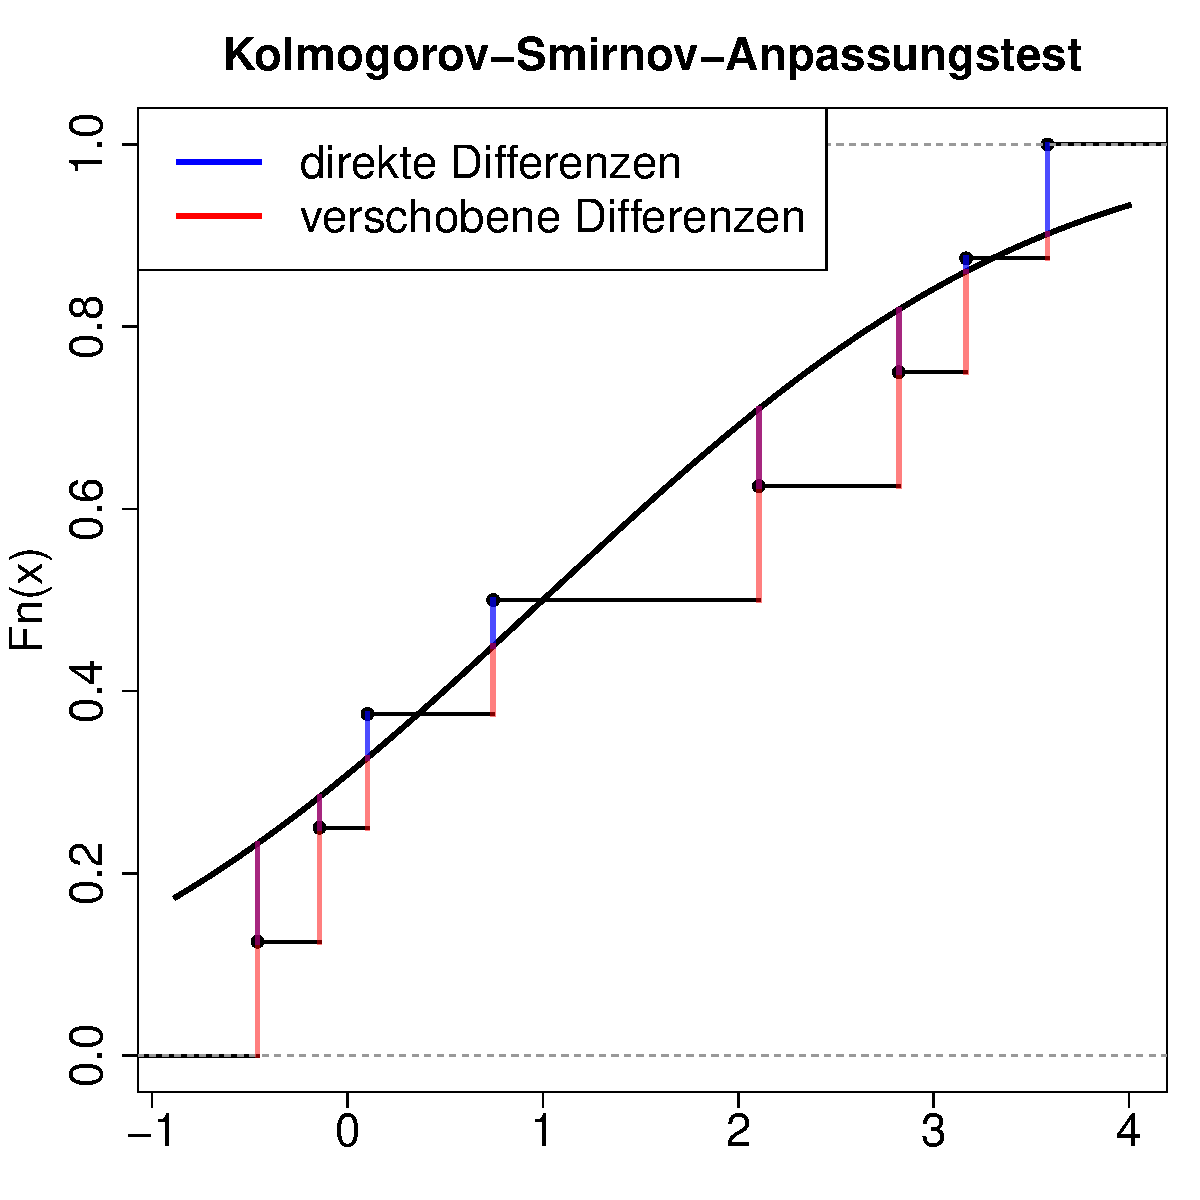
\includegraphics[width=8cm]{ks}
\vspace*{-1.5em}
\caption{Kolmogorov-Smirnov-Anpassungstest: Abweichungen zwischen kumulierten relativen Häufigkeiten der Daten und der Verteilungsfunktion der Normalverteilung $\mathcal{N}(\mu=1, \sigma=2)$}
\label{fig:ks}
\end{figure}

Der Kolmogorov-Smirnov-Test lässt sich auch verwenden, um die Daten einer stetigen Variable aus zwei Stichproben daraufhin zu prüfen, ob sie mit der $\text{H}_{0}$ verträglich sind, dass die Variable in beiden Bedingungen dieselbe Verteilung besitzt (Abschn.\ \ref{sec:ksoTest}).

%%%%%%%%%%%%%%%%%%%%%%%%%%%%%%%%%%%%%%%%%%%%%%%%%%%%%%%%%%%%%%%%%%
%%%%%%%%%%%%%%%%%%%%%%%%%%%%%%%%%%%%%%%%%%%%%%%%%%%%%%%%%%%%%%%%%%
\subsection[\texorpdfstring{$\chi^{2}$}{chi2}-Test auf eine feste Verteilung]{$\bm{\chi^{2}}$-Test auf eine feste Verteilung}
%%%%%%%%%%%%%%%%%%%%%%%%%%%%%%%%%%%%%%%%%%%%%%%%%%%%%%%%%%%%%%%%%%
%%%%%%%%%%%%%%%%%%%%%%%%%%%%%%%%%%%%%%%%%%%%%%%%%%%%%%%%%%%%%%%%%%

\index{Chi2-Test@$\chi^{2}$-Test!feste Verteilung}
Der $\chi^{2}$-Test auf eine feste Verteilung prüft Daten einer kategorialer Variable daraufhin, ob die empirischen Auftretenshäufigkeiten der einzelnen Kategorien verträglich mit einer theoretischen Verteilung unter $\text{H}_{0}$ sind, die die Wahrscheinlichkeit jeder Kategorie angibt.\footnote{Dieser Test ist auch bei quantitativen Variablen durchführbar, wobei zunächst eine Einteilung der Werte in disjunkte Klassen vorzunehmen ist. Die getestete $\text{H}_{0}$ ist dann in dem Sinne schwächer, dass alle Verteilungen äquivalent sind, die zu gleichen Klassenwahrscheinlichkeiten führen.} Als ungerichtete $\text{H}_{1}$ ergibt sich, dass die tatsächliche Verteilung nicht gleich der unter $\text{H}_{0}$ genannten\index[func]{chisq.test()@\lstinline{chisq.test()}} ist.
\begin{lstlisting}
chisq.test(x=<<Häufigkeiten>>, p=<<Wahrscheinlichkeiten>>,
           simulate.p.value=FALSE)
\end{lstlisting}

Unter \lstinline!x! ist der Vektor anzugeben, der die empirischen absoluten Auftretenshäufigkeiten der Kategorien beinhaltet. Dies kann z.\,B.\ eine Häufigkeitstabelle als Ergebnis von \lstinline!xtabs()! sein. Unter \lstinline!p! ist ein Vektor einzutragen, der die Wahrscheinlichkeiten für das Auftreten der Kategorien unter $\text{H}_{0}$ enthält und dieselbe Länge wie \lstinline!x! haben muss. Treten erwartete Häufigkeiten von Kategorien (das Produkt der Klassenwahrscheinlichkeiten mit der Stichprobengröße) $< 5$ auf, sollte das Argument \lstinline!simulate.p.value! auf \lstinline!TRUE! gesetzt werden. Andernfalls gibt R in einer solchen Situation die Warnung aus, dass die $\chi^{2}$-Approximation noch unzulänglich sein kann.

Als Beispiel soll ein empirischer Würfel daraufhin getestet werden, ob er fair ist. Die Auftretenswahrscheinlichkeit jeder Augenzahl unter $\text{H}_{0}$ beträgt $\frac{1}{6}$.
\begin{lstlisting}
> nRolls <- 50                                    # Anzahl Ziehungen
> nCateg <- 6                                     # Anzahl Kategorien
> pH0    <- rep(1/nCateg, nCateg)                 # Verteilung unter H0
> myData <- sample(1:nCateg, nRolls, replace=TRUE)   # simulierte Daten
> (tab   <- xtabs(~ myData))                      # Häufigkeiten
myData
1  2  3   4  5   6
8  8  4  14  3  13

> chisq.test(tab, p=pH0)
Chi-squared test for given probabilities
data: tab
X-squared = 12.16, df = 5, p-value = 0.03266
\end{lstlisting}

Die Ausgabe umfasst den Wert der mit wachsender Stichprobengröße asymptotisch $\chi^{2}$-verteilten Teststatistik (\lstinline!X-squared!) und ihre Freiheitsgrade (\lstinline!df!, nur wenn \lstinline!simulate.p.value! gleich \lstinline!FALSE! ist) samt zugehörigem $p$-Wert (\lstinline!p-value!). Das Ergebnis lässt sich manuell prüfen:
\begin{lstlisting}
> expected   <- pH0 * nRolls        # erwartete Häufigkeiten unter H0
> (statChisq <- sum((tab-expected)^2 / expected))   # Teststatistik
[1] 12.16

> (pVal <- pchisq(statChisq, nCateg-1, lower.tail=FALSE))   # p-Wert
[1] 0.03265998
\end{lstlisting}

%%%%%%%%%%%%%%%%%%%%%%%%%%%%%%%%%%%%%%%%%%%%%%%%%%%%%%%%%%%%%%%%%%
%%%%%%%%%%%%%%%%%%%%%%%%%%%%%%%%%%%%%%%%%%%%%%%%%%%%%%%%%%%%%%%%%%
\subsection[\texorpdfstring{$\chi^{2}$}{chi2}-Test auf eine Verteilungsklasse]{$\bm{\chi^{2}}$-Test auf eine Verteilungsklasse}
\label{sec:chisqGof}
%%%%%%%%%%%%%%%%%%%%%%%%%%%%%%%%%%%%%%%%%%%%%%%%%%%%%%%%%%%%%%%%%%
%%%%%%%%%%%%%%%%%%%%%%%%%%%%%%%%%%%%%%%%%%%%%%%%%%%%%%%%%%%%%%%%%%

\index{Chi2-Test@$\chi^{2}$-Test!Verteilungsklasse}
\index{Chi2-Test@$\chi^{2}$-Test!Normalverteilung}
\index{Verteilung!Normalverteilung!$\chi^{2}$-Test}
Als Spezialfall des $\chi^{2}$-Tests auf Gleichheit von Verteilungen (Abschn.\ \ref{sec:chisqEq}) kann die Verträglichkeit der Daten mit der $\text{H}_{0}$ getestet werden, dass die zugehörige theoretische Verteilung etwa aus der Familie der Normalverteilungen stammt -- andere Verteilungsfamilien lassen sich analog testen. Die $\text{H}_{1}$ ist ungerichtet, der Test asymptotisch korrekt bei wachsender Stichprobengröße und kann durch eine visuell-explorative Begutachtung eines Quantil-Quantil-Diagramms ergänzt werden (Abschn.\ \ref{sec:qq}).

Die Daten sind zunächst in disjunkte Klassen einzuteilen, deren empirische Auftretenshäufigkeiten mit den unter $\text{H}_{0}$ erwarteten verglichen werden.\footnote{Die Klassenbildung führt dazu, dass statt der Verträglichkeit mit einer bestimmten Verteilung die schwächere $\text{H}_{0}$ einer Verträglichkeit mit allen Verteilungen getestet wird, die zu denselben erwarteten Häufigkeiten führen.} Die Parameter der konkreten Normalverteilung unter $\text{H}_{0}$ folgen entweder aus theoretischen Erwägungen oder werden auf Basis der Daten geschätzt, häufig anhand des Mittelwertes und der korrigierten Stichprobenstreuung. Durch eine solche Schätzung beider Parameter aus den Daten reduziert sich die Anzahl der Freiheitsgrade beim Test um $2$.\footnote{Für eine korrekte Testkonstruktion wäre eigentlich eine feste Klasseneinteilung mit gruppierter Maximum-Likelihood- oder Minimum-$\chi^{2}$-Schätzung von $\mu$ und $\sigma$ notwendig, die in Abschn.\ \ref{sec:optim} demonstriert wird.}

Das Paket \lstinline!DescTools!\index[pack]{DescTools@\lstinline{DescTools}} enthält mit \lstinline!PearsonTest()!\index[func]{PearsonTest()@\lstinline{PearsonTest()}} eine Funktion für den $\chi^{2}$-Test auf Normalverteiltheit, über die sowohl die Klasseneinteilung wie auch die Korrektur der Freiheitsgrade per Argument festgelegt werden können.
\begin{lstlisting}
PearsonTest(x=<<Vektor>>, n.classes=<<Anzahl>>, adjust=TRUE)
\end{lstlisting}

Der Datenvektor wird der Funktion als Argument \lstinline!x! übergeben, \lstinline!n.classes! legt die Zahl der zu bildenden Klassen fest. Die Funktion wählt die genaue Lage der Klassengrenzen so, dass alle Klassen unter $\text{H}_{0}$ dieselbe Wahrscheinlichkeit besitzen. Über \lstinline!adjust! wird angegeben, ob die Zahl der Freiheitsgrade in Folge einer Schätzung der Parameter der Normalverteilung unter $\text{H}_{0}$ aus den Daten um $2$ nach unten zu korrigieren ist.

\begin{lstlisting}
> DV   <- rnorm(100, mean=100, sd=15)             # simulierte Daten
> nCls <- 6                                       # Anzahl Klassen
> library(DescTools)                              # für PearsonTest()
> PearsonTest(DV, n.classes=nCls, adjust=TRUE)
Pearson chi-square normality test
data: DV
P = 3.08, p-value = 0.3795
\end{lstlisting}

Die Ausgabe nennt den empirischen $\chi^{2}$-Wert unter \lstinline!P! zusammen mit dem zugehörigen $p$-Wert. Für einen manuellen Test sollen ebenfalls unter $\text{H}_{0}$ gleichwahrscheinliche Intervalle als Basis dienen. Deren innere Grenzen liefert \lstinline!qnorm()!, wobei Erwartungswert und Streuung aus den Daten geschätzt werden.
\begin{lstlisting}
# innere Intervallgrenzen für gleichwahrscheinliche Intervalle
> limits <- qnorm(seq(1/nCls, (nCls-1)/nCls, length.out=nCls-1),
+                 mean(DV), sd(DV))

> DVcut    <- cut(DV, c(-Inf, limits, Inf))  # +äußere Intervallgrenzen
> (intFreq <- xtabs(~ DVcut))                # beobachtete Häufigkeiten
DVcut
(-Inf,87.3]  (87.3,95.1]  (95.1,101]  (101,108]  (108,115]  (115, Inf]
         19           14          14         16         22          15
\end{lstlisting}

Beim Vergleich von beobachteten und erwarteten Klassenhäufigkeiten ist zu berücksichtigen, dass der von \lstinline!chisq.test()! ausgegebene $p$-Wert nicht die Reduktion der Freiheitsgrade widerspiegelt und deshalb für diesen Test nicht der richtige ist. Ist \lstinline!<<Objekt>>! das Ergebnis von \lstinline!chisq.test()!, muss die Bestimmung des korrekten $p$-Wertes manuell mit dem empirischen Wert der Teststatistik, den richtigen Freiheitsgraden und der Verteilungsfunktion \lstinline!pchisq(<<Quantil>>, <<Freiheitsgrade>>)! erfolgen.
\begin{lstlisting}
# Test für gleiche Klassenwahrscheinlichkeiten, falsche Freiheitsgrade
> (resChisq <- chisq.test(intFreq, p=rep(1/nCls, nCls)))
Chi-squared test for given probabilities
data: intFreq
X-squared = 3.08, df = 5, p-value = 0.6877

# Test mit den richtigen Freiheitsgraden
> statChisq <- resChisq$statistic          # Teststatistik chi^2
> realDf    <- resChisq$parameter - 2      # korrigierte Freiheitsgrade

# korrigierter p-Wert
> (realPval <- pchisq(statChisq, realDf, lower.tail=FALSE))
0.3794545
\end{lstlisting}

%%%%%%%%%%%%%%%%%%%%%%%%%%%%%%%%%%%%%%%%%%%%%%%%%%%%%%%%%%%%%%%%%%
%%%%%%%%%%%%%%%%%%%%%%%%%%%%%%%%%%%%%%%%%%%%%%%%%%%%%%%%%%%%%%%%%%
\section{Analyse von gemeinsamen Häufigkeiten kategorialer Variablen}
\label{sec:freqNonparam}
%%%%%%%%%%%%%%%%%%%%%%%%%%%%%%%%%%%%%%%%%%%%%%%%%%%%%%%%%%%%%%%%%%
%%%%%%%%%%%%%%%%%%%%%%%%%%%%%%%%%%%%%%%%%%%%%%%%%%%%%%%%%%%%%%%%%%

Inwieweit die gemeinsamen empirischen Auftretenshäufigkeiten der Ausprägungen kategorialer Variablen theoretischen Vorstellungen entsprechen, kann durch folgende Tests geprüft werden. Sie ergänzen die in Kap.\ \ref{sec:glm} vorgestellten Regressionsmodelle für bestimmte Spezialfälle.

%%%%%%%%%%%%%%%%%%%%%%%%%%%%%%%%%%%%%%%%%%%%%%%%%%%%%%%%%%%%%%%%%%
%%%%%%%%%%%%%%%%%%%%%%%%%%%%%%%%%%%%%%%%%%%%%%%%%%%%%%%%%%%%%%%%%%
\subsection[\texorpdfstring{$\chi^{2}$}{chi2}-Test auf Unabhängigkeit]{$\bm{\chi^{2}}$-Test auf Unabhängigkeit}
\label{sec:chisqInd}
%%%%%%%%%%%%%%%%%%%%%%%%%%%%%%%%%%%%%%%%%%%%%%%%%%%%%%%%%%%%%%%%%%
%%%%%%%%%%%%%%%%%%%%%%%%%%%%%%%%%%%%%%%%%%%%%%%%%%%%%%%%%%%%%%%%%%

\index{Chi2-Test@$\chi^{2}$-Test!Unabhängigkeit}
Beim $\chi^{2}$-Test auf Unabhängigkeit wird die empirische Kontingenztafel von zwei an derselben Stichprobe erhobenen kategorialen Variablen daraufhin geprüft, ob sie verträglich mit der $\text{H}_{0}$ ist, dass beide Variablen unabhängig sind.\footnote{Dieser Test ist auch bei quantitativen Variablen durchführbar, wobei zunächst eine Einteilung der Werte in disjunkte Klassen vorzunehmen ist. Die getestete $\text{H}_{0}$ ist dann in dem Sinne schwächer, dass nur die Unabhängigkeit bzgl.\ der vorgenommenen Klasseneinteilung getestet wird.} Die $\text{H}_{1}$ ist ungerichtet, der Test asymptotisch korrekt bei wachsender\index[func]{chisq.test()@\lstinline{chisq.test()}} Stichprobengröße.
\begin{lstlisting}
chisq.test(x, y=NULL, simulate.p.value=FALSE)
\end{lstlisting}

Unter \lstinline!x! kann eine zweidimensionale Kontingenztafel eingegeben werden -- etwa als Ergebnis von \lstinline!xtabs(~ <<Faktor1>> + <<Faktor2>>)!, oder als Matrix mit den Häufigkeiten der Stufenkombinationen zweier Variablen. Alternativ kann \lstinline!x! ein Objekt der Klasse \lstinline!factor! mit den Ausprägungen der ersten Variable sein. In diesem Fall muss auch \lstinline!y! angegeben werden, das dann ebenfalls ein Objekt der Klasse \lstinline!factor! derselben Länge wie \lstinline!x! mit an denselben Beobachtungsobjekten erhobenen Daten zu sein hat.

Unter $\text{H}_{0}$ ergeben sich die Zellwahrscheinlichkeiten jeweils als Produkt der zugehörigen Randwahrscheinlichkeiten, die über die relativen Randhäufigkeiten geschätzt werden. Das Argument \lstinline!simulate.p.value=TRUE! sollte gesetzt werden, wenn erwartete Zellhäufigkeiten $< 5$ auftreten. Andernfalls gibt R in einer solchen Situation die Warnung aus, dass die $\chi^{2}$-Approximation noch unzulänglich sein kann.

Als Beispiel sei eine Stichprobe von Studenten betrachtet, die angeben, ob sie rauchen und wie viele Geschwister sie haben.
\begin{lstlisting}
> N        <- 50                           # Stichprobengröße
> smokes   <- factor(sample(c("no", "yes"), N, replace=TRUE))
> siblings <- factor(round(abs(rnorm(N, 1, 0.5))))
> cTab     <- xtabs(~ smokes + siblings)   # Kontingenztafel
> addmargins(cTab)                         # Randsummen
           siblings
smokes  0   1  2  Sum
    no  6  18  1   25
   yes  2  18  5   25
   Sum  8  36  6   50

> chisq.test(cTab)
Pearson's Chi-squared test
data: cTab
X-squared = 4.6667, df = 2, p-value = 0.09697

Warning message:
In chisq.test(cTab) : Chi-squared approximation may be incorrect
\end{lstlisting}

Das Ergebnis lässt sich manuell kontrollieren:
\begin{lstlisting}
> P <- nlevels(smokes)                     # Anzahl smokes Kategorien
> Q <- nlevels(siblings)                   # Anzahl siblings Kategorien

# erwartete Häufigkeiten -> alle Produkte der Randhäufigkeiten
# relativiert an der Summe von Beobachtungen
> expected   <- outer(rowSums(cTab), colSums(cTab)) / sum(cTab)
> (statChisq <- sum((cTab-expected)^2 / expected))      # Teststatistik
[1] 4.666667

> (pVal <- pchisq(statChisq, (P-1)*(Q-1), lower.tail=FALSE))  # p-Wert
[1] 0.09697197
\end{lstlisting}

Siehe Abschn.\ \ref{sec:loglin} für eine Verallgemeinerung zur Analyse höherdimensionaler Kontingenztafeln absoluter Häufigkeiten mit Hilfe log-linearer Modelle.

%%%%%%%%%%%%%%%%%%%%%%%%%%%%%%%%%%%%%%%%%%%%%%%%%%%%%%%%%%%%%%%%%%
%%%%%%%%%%%%%%%%%%%%%%%%%%%%%%%%%%%%%%%%%%%%%%%%%%%%%%%%%%%%%%%%%%
\subsection[\texorpdfstring{$\chi^{2}$}{chi2}-Test auf Gleichheit von Verteilungen]{$\bm{\chi^{2}}$-Test auf Gleichheit von Verteilungen}
\label{sec:chisqEq}
%%%%%%%%%%%%%%%%%%%%%%%%%%%%%%%%%%%%%%%%%%%%%%%%%%%%%%%%%%%%%%%%%%
%%%%%%%%%%%%%%%%%%%%%%%%%%%%%%%%%%%%%%%%%%%%%%%%%%%%%%%%%%%%%%%%%%

\index{Chi2-Test@$\chi^{2}$-Test!Gleichheit von Verteilungen}
Beim $\chi^{2}$-Test auf Gleichheit von bedingten Verteilungen werden die empirischen eindimensionalen Häufigkeitsverteilungen einer kategorialen Variable in unterschiedlichen Stichproben daraufhin geprüft, ob sie mit der $\text{H}_{0}$ verträglich sind, dass ihre Stufen in allen Bedingungen jeweils dieselben Auftretenswahrscheinlichkeiten besitzen.\footnote{Dieser Test ist auch bei quantitativen Variablen durchführbar, wobei zunächst eine Einteilung der Werte in disjunkte Klassen vorzunehmen ist. Die getestete $\text{H}_{0}$ ist dann in dem Sinne schwächer, dass nur die Gleichheit der Verteilungen bzgl.\ der vorgenommenen Klasseneinteilung getestet wird.} Die $\text{H}_{1}$ ist ungerichtet, der Test asymptotisch korrekt bei wachsender Stichprobengröße. Getestet wird wie in Abschn.\ \ref{sec:chisqInd} mit \lstinline!chisq.test()! auf Basis der Kontingenztafel gemeinsamer Häufigkeiten.

Als Beispiel soll die politische Orientierung von $100$ Studenten aus zwei Studiengängen getestet werden. AV sei die gewählte von fünf Parteien.
\begin{lstlisting}
> voteX <- rep(LETTERS[1:5], c(3,  8, 12, 19, 8))   # Ergebnisse Fach X
> voteY <- rep(LETTERS[1:5], c(8, 17, 16,  7, 2))   # Ergebnisse Fach Y
> vote  <- c(voteX, voteY)                          # beide Ergebnisse

# entsprechender Faktor mit Gruppenzugehörigkeiten
> studies <- factor(rep(c("X", "Y"), c(length(voteX), length(voteY))))
> cTab    <- xtabs(~ studies + vote)                # Kontingenztafel
> addmargins(cTab)                                  # Randsummen
                vote
studies   A   B   C   D   E  Sum
      X   3   8  12  19   8   50
      Y   8  17  16   7   2   50
    Sum  11  25  28  26  10  100

# simulate.p.value=TRUE wegen geringen erwarteten Häufigkeiten
> chisq.test(cTab, simulate.p.value=TRUE)
Pearson's Chi-squared test with simulated p-value
(based on 2000 replicates)
data: cTab
X-squared = 15.2226, df = NA, p-value = 0.005497
\end{lstlisting}

%%%%%%%%%%%%%%%%%%%%%%%%%%%%%%%%%%%%%%%%%%%%%%%%%%%%%%%%%%%%%%%%%%
%%%%%%%%%%%%%%%%%%%%%%%%%%%%%%%%%%%%%%%%%%%%%%%%%%%%%%%%%%%%%%%%%%
\subsection[\texorpdfstring{$\chi^{2}$}{chi2}-Test für mehrere Auftretenswahrscheinlichkeiten]{$\bm{\chi^{2}}$-Test für mehrere Auftretenswahrscheinlichkeiten}
\label{sec:propTest}
%%%%%%%%%%%%%%%%%%%%%%%%%%%%%%%%%%%%%%%%%%%%%%%%%%%%%%%%%%%%%%%%%%
%%%%%%%%%%%%%%%%%%%%%%%%%%%%%%%%%%%%%%%%%%%%%%%%%%%%%%%%%%%%%%%%%%

\index{Chi2-Test@$\chi^{2}$-Test!Auftretenswahrscheinlichkeiten}
Für eine in mehr als einer Bedingung erhobene dichotome Variable prüft\index[func]{prop.test()@\lstinline{prop.test()}} \lstinline!prop.test()!, ob die Trefferwahrscheinlichkeit in allen Bedingungen dieselbe ist. Es handelt sich also um eine Hypothese zur Gleichheit von Verteilungen einer dichotomen Variable in mehreren Bedingungen. Der Test ist asymptotisch korrekt bei wachsender Stichprobengröße, die $\text{H}_{1}$ ist ungerichtet.
\begin{lstlisting}
prop.test(x=<<Erfolge>>, n=<<Stichprobenumfänge>>)
\end{lstlisting}

Die Argumente \lstinline!x! und \lstinline!n! beziehen sich auf die Anzahl der Treffer und die Stichprobengrößen in den Gruppen. Für sie können Vektoren gleicher Länge mit Einträgen für jede Gruppe angegeben werden. Anstelle von \lstinline!x! und \lstinline!n! ist auch eine Matrix mit zwei Spalten möglich, die in jeder Zeile die Zahl der Treffer und Nicht-Treffer für jeweils eine Gruppe enthält.
\begin{lstlisting}
> total <- c(5000, 5000, 5000)                      # Gruppengrößen
> hits  <- c(585, 610, 539)                         # Anzahl Treffer
> prop.test(hits, total)
3-sample test for equality of proportions without continuity correction
data: hits out of total
X-squared = 5.0745, df = 2, p-value = 0.07908
alternative hypothesis: two.sided
sample estimates:
prop 1  prop 2  prop 3
0.1170  0.1220  0.1078
\end{lstlisting}

Die Ausgabe berichtet den Wert der $\chi^{2}$-Teststatistik (\lstinline!X-squared!) samt des zugehörigen $p$-Wertes (\lstinline!p-value!) zusammen mit den Freiheitsgraden (\lstinline!df!) und schließlich die relativen Erfolgshäufigkeiten in den Gruppen (\lstinline!sample estimates!). Dasselbe Ergebnis lässt sich auch durch geeignete Anwendung des $\chi^{2}$-Tests auf Gleichheit von Verteilungen erzielen. Hierfür müssen zunächst für jede der drei Stichproben auch die Auftretenshäufigkeiten der zweiten Kategorie berechnet und zusammen mit jenen der ersten Kategorie in einer Matrix zusammengestellt werden.
\begin{lstlisting}
> (mat <- cbind(hits, total-hits))     # Matrix mit Treffern und Nieten
     [,1]  [,2]
[1,]  585  4415
[2,]  610  4390
[3,]  539  4461

> chisq.test(mat)
Pearson's Chi-squared test
data: mat
X-squared = 5.0745, df = 2, p-value = 0.07908
\end{lstlisting}

Ergeben sich die Gruppen durch Ausprägungen einer ordinalen Variable, ist mit \lstinline!prop.trend.test()!\index[func]{prop.trend.test()@\lstinline{prop.trend.test()}} ebenfalls über eine $\chi^{2}$-Teststatistik die spezialisiertere Prüfung möglich, ob die Erfolgswahrscheinlichkeiten der dichotomen Variable einem Trend bzgl.\ der ordinalen Variable folgen.

%%%%%%%%%%%%%%%%%%%%%%%%%%%%%%%%%%%%%%%%%%%%%%%%%%%%%%%%%%%%%%%%%%
%%%%%%%%%%%%%%%%%%%%%%%%%%%%%%%%%%%%%%%%%%%%%%%%%%%%%%%%%%%%%%%%%%
\subsection{Fishers exakter Test auf Unabhängigkeit}
\label{sec:fisherInd}
%%%%%%%%%%%%%%%%%%%%%%%%%%%%%%%%%%%%%%%%%%%%%%%%%%%%%%%%%%%%%%%%%%
%%%%%%%%%%%%%%%%%%%%%%%%%%%%%%%%%%%%%%%%%%%%%%%%%%%%%%%%%%%%%%%%%%

\index{Fishers exakter Test!Unabhängigkeit}
Werden zwei dichotome Variablen in einer Stichprobe erhoben, kann mit Fishers exaktem Test die $\text{H}_{0}$ geprüft werden, dass beide Variablen unabhängig sind.\footnote{\label{ftn:oddsRatio}Die $\text{H}_{0}$ ist äquivalent zur Hypothese, dass das wahre \emph{odds ratio} der Kontingenztafel beider Variablen gleich $1$ ist (Abschn.\ \ref{sec:confMat}). Der Test lässt sich auf Variablen mit mehr als zwei Stufen verallgemeinern, vgl.\ \lstinline!?fisher.test!.} Anders als beim $\chi^{2}$-Test zur selben Hypothese sind hier auch gerichtete Alternativhypothesen über den Zusammenhang\index[func]{fisher.test()@\lstinline{fisher.test()}} möglich.
\begin{lstlisting}
fisher.test(x, y=NULL, conf.level=0.95,
            alternative=c("two.sided", "less", "greater"))
\end{lstlisting}

Unter \lstinline!x! ist entweder die $(2 \times 2)$-Kontingenztafel zweier dichotomer Variablen oder ein Objekt der Klasse \lstinline!factor! mit zwei Stufen anzugeben, das die Ausprägungen der ersten dichotomen Variable enthält. In diesem Fall muss auch ein Faktor \lstinline!y! mit zwei Stufen und derselben Länge wie \lstinline!x! angegeben werden, der Daten derselben Beobachtungsobjekte beinhaltet. Das Argument \lstinline!alternative! bestimmt, ob zweiseitig, links- oder rechtsseitig getestet werden soll. Die Richtung der Fragestellung bezieht sich dabei auf die Größe des \emph{odds ratio} (OR) in der theoretischen Kontingenztafel. Linksseitiges Testen bedeutet, dass unter $\text{H}_{1}$ OR $< 1$ ist (negativer Zusammenhang), rechtsseitiges Testen entsprechend, OR $> 1$ (positiver Zusammenhang). Mit dem Argument \lstinline!conf.level! wird die Breite des Konfidenzintervalls für das OR festgelegt.

Im Beispiel soll geprüft werden, ob das Ergebnis eines diagnostischen Instruments für eine bestimmte Krankheit wie gewünscht positiv mit dem Vorliegen dieser Krankheit zusammenhängt.
\begin{lstlisting}
# Gruppenzugehörigkeit: 10 Gesunde, 5 Kranke
> disease <- factor(rep(c("no", "yes"), c(10, 5)))
> diagN   <- rep(c("isHealthy", "isIll"), c(8, 2)) # Diagnose für Gesunde
> diagY   <- rep(c("isHealthy", "isIll"), c(1, 4)) # Diagnose für Kranke
> diagT   <- factor(c(diagN, diagY))               # alle Diagnosen
> contT1  <- xtabs(~ disease + diagT)              # Kontingenztafel
> addmargins(contT1)                               # Randsummen
                 diagT
disease  isHealthy  isIll  Sum
     no          8      2   10
    yes          1      4    5
    Sum          9      6   15

> fisher.test(contT1, alternative="greater")
Fisher's Exact Test for Count Data
data: contT1
p-value = 0.04695
alternative hypothesis: true odds ratio is greater than 1
95 percent confidence interval:
1.031491  Inf
sample estimates:
odds ratio
12.49706
\end{lstlisting}

Die Ausgabe enthält neben dem $p$-Wert (\lstinline!p-value!) das Konfidenzintervall für das OR in der gewünschten Breite sowie die bedingte Maximum-Likelihood-Schätzung des OR für die gegebenen Randhäufigkeiten (\lstinline!sample estimates!). Der $p$-Wert lässt sich manuell nachprüfen: Als Variante eines Permutationstests (Abschn.\ \ref{sec:permTests}) müssen hierfür die Punktwahrscheinlichkeiten für die vorliegende sowie für i.\,S.\ der $\text{H}_{1}$ extremere Kontingenztafeln bei gleichen Randhäufigkeiten mit der hypergeometrischen Verteilung ermittelt und summiert werden. Im gegebenen Fall besteht nur eine Möglichkeit, die Kontingenztafel extremer zu machen, ohne die Randhäufigkeiten zu ändern.
\begin{lstlisting}
# Punktwahrscheinlichkeit für die gegebene Kontingenztafel
> (p1 <- dhyper(8, 8+2, 1+4, 8+1))
[1] 0.04495504

# Punktwahrscheinlichkeit für extremere Kontingenztafel
> (p2 <- dhyper(9, 9+1, 0+5, 9+0))
[1] 0.001998002

> (pVal <- p1 + p2)     # Summe der Punktwahrscheinlichkeiten -> p-Wert
[1] 0.04695305
\end{lstlisting}

Die $\text{H}_{0}$, dass zwei dichotome Variablen in mehreren, durch eine dritte kategoriale Variable gebildeten Bedingungen jeweils unabhängig sind, prüft der\index{Cochran-Mantel-Hänszel-Test} Cochran-Mantel-Hänszel-Test, für den die Funktion\index[func]{mantelhaen.test()@\lstinline{mantelhaen.test()}} \lstinline!mantelhaen.test()! existiert. Sie ist auch im allgemeineren Fall anwendbar, dass die Unabhängigkeit kategorialer Variablen mit mehr als zwei Stufen zu testen ist.

%%%%%%%%%%%%%%%%%%%%%%%%%%%%%%%%%%%%%%%%%%%%%%%%%%%%%%%%%%%%%%%%%%
%%%%%%%%%%%%%%%%%%%%%%%%%%%%%%%%%%%%%%%%%%%%%%%%%%%%%%%%%%%%%%%%%%
\subsection{Fishers exakter Test auf Gleichheit von Verteilungen}
\label{sec:fisherEq}
%%%%%%%%%%%%%%%%%%%%%%%%%%%%%%%%%%%%%%%%%%%%%%%%%%%%%%%%%%%%%%%%%%
%%%%%%%%%%%%%%%%%%%%%%%%%%%%%%%%%%%%%%%%%%%%%%%%%%%%%%%%%%%%%%%%%%

\index{Fishers exakter Test!Gleichheit von Verteilungen}
Für Daten einer dichotomen Variable aus zwei unabhängigen Stichproben prüft Fishers exakter Test die $\text{H}_{0}$, dass die Variablen in beiden Bedingungen identische Erfolgswahrscheinlichkeit besitzen. Anders als beim $\chi^{2}$-Test zur selben Hypothese sind hier auch gerichtete Alternativhypothesen möglich.

Der Aufruf von \lstinline!fisher.test()!\index[func]{fisher.test()@\lstinline{fisher.test()}} ist identisch zu jenem beim Test auf Unabhängigkeit (vgl.\ auch Fußnote \ref{ftn:oddsRatio}). Unter \lstinline!x! ist hier entweder die $(2 \times 2)$-Kontingenztafel einer dichotomen Zufallsvariable und eines Gruppierungsfaktors mit zwei Ausprägungen anzugeben oder ein Objekt der Klasse \lstinline!factor! mit zwei Stufen, das die Ausprägungen der Variable in der ersten Stichprobe enthält. In letzterem Fall muss auch ein Faktor \lstinline!y! mit zwei Stufen und derselben Länge wie \lstinline!x! angegeben werden, der Daten derselben Variable aus einer zweiten Stichprobe beinhaltet.

Im Beispiel sei an je einer Stichprobe aus der Population der Frauen und der Männer erhoben worden, ob die Person raucht. Geprüft wird die $\text{H}_{0}$, dass der Anteil der Raucher in beiden Populationen gleich ist, wobei als $\text{H}_{1}$ hier vermutet wird, dass Frauen generell häufiger rauchen. Der Aufbau der Kontingenztafel verlangt nach einem linksseitigen Test.
\begin{lstlisting}
> N          <- 20                                # Stichprobengröße
> smokesFem  <- rbinom(N, size=1, p=0.6)          # Daten Frauen
> smokesMale <- rbinom(N, size=1, p=0.4)          # Daten Männer

# Faktoren, die Rauchverhalten und Geschlecht codieren
> smokes <- factor(c(smokesFem, smokesMale), labels=c("no", "yes"))
> sex    <- factor(rep(c("f", "m"), each=N))      # Faktor Geschlecht
> contT2 <- xtabs(~ sex + smokes)                 # Kontingenztafel
> addmargins(contT2)                              # Randsummen
        smokes
sex  no  yes  Sum
  f   8   12   20
  m  16    4   20
Sum  24   16   40

> fisher.test(contT2, alternative="less")
Fisher's Exact Test for Count Data
data: contT2
p-value = 0.01124
alternative hypothesis: true odds ratio is less than 1
95 percent confidence interval:
0.0000000  0.6668953
sample estimates:
odds ratio
0.1751986
\end{lstlisting}

%%%%%%%%%%%%%%%%%%%%%%%%%%%%%%%%%%%%%%%%%%%%%%%%%%%%%%%%%%%%%%%%%%
%%%%%%%%%%%%%%%%%%%%%%%%%%%%%%%%%%%%%%%%%%%%%%%%%%%%%%%%%%%%%%%%%%
\subsection[Kennwerte von \texorpdfstring{$(2 \times 2)$}{(2x2)}-Konfusionsmatrizen]{Kennwerte von \bm{$(2 \times 2)$}-Konfusionsmatrizen}
\label{sec:confMat}
%%%%%%%%%%%%%%%%%%%%%%%%%%%%%%%%%%%%%%%%%%%%%%%%%%%%%%%%%%%%%%%%%%
%%%%%%%%%%%%%%%%%%%%%%%%%%%%%%%%%%%%%%%%%%%%%%%%%%%%%%%%%%%%%%%%%%

\index{2x2@$(2 \times 2)$-Kontingenztafel}
\index{Konfusionsmatrix}
$(2 \times 2)$-Kontingenztafeln als Ergebnis einer zweifachen dichotomen Klassifikation (\emph{Konfusionsmatrizen}) erlauben die Berechnung mehrerer Kennwerte, um Eigenschaften der Klassifikation zu beschreiben. Hierzu zählen die Sensitivität, Spezifität und Relevanz sowie das odds ratio und das relative Risiko.\footnote{Das Paket\index[pack]{riskyr@\lstinline{riskyr}} \lstinline!riskyr! \cite{Neth2019} stellt eine Vielzahl von Auswertungsfunktionen und Diagrammen zur Analyse sowie zum besseren Verständnis von Konfusionsmatrizen bereit.}

Als Beispiel seien die Daten herangezogen, die bereits für Fishers exakten Test auf Unabhängigkeit verwendet wurden. Dabei sollen die Abkürzungen TP (\emph{true positive, hit}) für richtig positive, TN (\emph{true negative}) für richtig negative, FP (\emph{false positive}) für falsch positive und FN (\emph{false negative, miss}) für falsch negative Diagnosen stehen.
\begin{lstlisting}
> addmargins(contT1)
                 diagT              #              Diagnose
disease  isHealthy  isIll  Sum      # krank?  "gesund"   "krank"
     no          8      2   10      #   nein     TN         FP
    yes          1      4    5      #     ja     FN         TP
    Sum          9      6   15

> TN <- contT1[1, 1]                # true negative
> TP <- contT1[2, 2]                # true positive / hit
> FP <- contT1[1, 2]                # false positive
> FN <- contT1[2, 1]                # false negative / miss
\end{lstlisting}

%%%%%%%%%%%%%%%%%%%%%%%%%%%%%%%%%%%%%%%%%%%%%%%%%%%%%%%%%%%%%%%%%%
%%%%%%%%%%%%%%%%%%%%%%%%%%%%%%%%%%%%%%%%%%%%%%%%%%%%%%%%%%%%%%%%%%
\subsubsection{Sensitivität, Spezifität und Relevanz}
%%%%%%%%%%%%%%%%%%%%%%%%%%%%%%%%%%%%%%%%%%%%%%%%%%%%%%%%%%%%%%%%%%
%%%%%%%%%%%%%%%%%%%%%%%%%%%%%%%%%%%%%%%%%%%%%%%%%%%%%%%%%%%%%%%%%%

Der Basisumfang von R stellt zur Ermittlung der folgenden Kennwerte keine eigene Funktion bereit, eine manuelle Berechnung ist jedoch unkompliziert. Die Prävalenz\index{Prävalenz|see{$(2 \times 2)$-Kontingenztafel}} der Krankheit ist der Anteil der Kranken an der Gesamtzahl von Beobachtungen. Im Kontext des Satzes von Bayes entspricht dies der a-priori Wahrscheinlichkeit eines Merkmals.
\begin{lstlisting}
> (prevalence <- sum(contT1[2, ]) / sum(contT1))
[1] 0.3333333
\end{lstlisting}

Die\index{Sensitivität|see{$(2 \times 2)$-Kontingenztafel}} Sensitivität, in anderem Kontext auch \emph{recall}\index{recall|see{$(2 \times 2)$-Kontingenztafel}} genannt, ist TP / (TP + FN), also das Verhältnis von richtig entdeckten zu allen zu entdeckenden Elementen. In der Sprechweise inferenzstatistischer Tests wäre dies auf theoretischer Ebene die power eines Tests. Entsprechend wäre die Wahrscheinlichkeit eines Fehlers zweiter Art ($\beta$) gleich $1-\text{Sensitivität}$.
\begin{lstlisting}
> (sensitivity <- recall <- TP / (TP+FN))
[1] 0.8
\end{lstlisting}

Die Spezifität\index{Spezifität|see{$(2 \times 2)$-Kontingenztafel}} ist TN / (TN + FP), also hier das Verhältnis von richtig als gesund Eingestuften zu allen Gesunden. In der Sprechweise inferenzstatistischer Tests wäre $1 - \text{Spezifität}$ auf theoretischer Ebene gleich der Wahrscheinlichkeit eines Fehlers erster Art ($\alpha$), dem somit $\frac{\text{FP}}{\text{TN} + \text{FP}}$ entspräche.
\begin{lstlisting}
> (specificity <- TN / (TN+FP))
[1] 0.8
\end{lstlisting}

Die\index{Relevanz|see{$(2 \times 2)$-Kontingenztafel}} Relevanz, je nach Kontext auch als\index{Präzision|see{$(2 \times 2)$-Kontingenztafel}} Präzision oder\index{positiver Vorhersagewert|see{$(2 \times 2)$-Kontingenztafel}} positiver Vorhersagewert bezeichnet, ist TP / (TP + FP). Er gibt damit hier an, welcher Anteil der als krank Diagnostizierten tatsächlich krank ist. Im Kontext des Satzes von Bayes entspricht dies der a-posteriori Wahrscheinlichkeit eines Merkmals gegeben die positive Diagnose.
\begin{lstlisting}
> (relevance <- precision <- ppv <- TP / (TP+FP))
[1] 0.6666667
\end{lstlisting}

Der Anteil richtiger Diagnosen an allen Diagnosen wird auch als Rate der korrekten Klassifikation\index{Rate der korrekten Klassifikation|see{$(2 \times 2)$-Kontingenztafel}} bezeichnet und ist der Quotient aus der Summe der Diagonalelemente und der Summe aller Elemente.
\begin{lstlisting}
> (CCR <- sum(diag(contT1)) / sum(contT1))
[1] 0.8
\end{lstlisting}

Das\index{F-Mass@$F$-Maß|see{$(2 \times 2)$-Kontingenztafel}} $F$-Maß als harmonisches Mittel von Präzision und recall wird bisweilen als integriertes Gütemaß für eine Klassifikation herangezogen. Er ist nicht mit Werten einer $F$-Verteilung zu verwechseln.
\begin{lstlisting}
> (Fval <- 1 / mean(1 / c(precision, recall)))
[1] 0.7272727
\end{lstlisting}

%%%%%%%%%%%%%%%%%%%%%%%%%%%%%%%%%%%%%%%%%%%%%%%%%%%%%%%%%%%%%%%%%%
%%%%%%%%%%%%%%%%%%%%%%%%%%%%%%%%%%%%%%%%%%%%%%%%%%%%%%%%%%%%%%%%%%
\subsubsection{Odds ratio, Yules $\bm{Q}$ und relatives Risiko}
%%%%%%%%%%%%%%%%%%%%%%%%%%%%%%%%%%%%%%%%%%%%%%%%%%%%%%%%%%%%%%%%%%
%%%%%%%%%%%%%%%%%%%%%%%%%%%%%%%%%%%%%%%%%%%%%%%%%%%%%%%%%%%%%%%%%%

\index{odds ratio}
\index{Chancenverhältnis}
\index{Yules Q-Koeffizient@Yules $Q$-Koeffizient}
\index{Q-Koeffizient@$Q$-Koeffizient|see{Yules $Q$-Koeffizient}}
Das odds ratio (OR, Chancenverhältnis) ist ein Zusammenhangsmaß für zwei dichotome Variablen und ergibt sich aus der $(2 \times 2)$-Kontingenztafel ihrer gemeinsamen Häufigkeiten: $\left( \begin{smallmatrix} a & b\\ c & d \end{smallmatrix} \right)$. %
%$\left( \begin{array}{cc} a & b\\ c & d \end{array} \right)$.%
Das OR berechnet sich durch Division der \emph{Wettquotienten} (Chancen) $\frac{a}{b}$ und $\frac{c}{d}$, also als $\frac{a \cdot d}{b \cdot c}$. Repräsentieren die Zeilen der Kontingenztafel zwei Bedingungen und die Spalten die An- bzw.\ Abwesenheit eines Merkmals, drückt das OR die multiplikative Änderung der bedingten Verteilung des Merkmals beim Wechsel der Bedingungen aus.

Das OR lässt sich manuell, oder alternativ über\index[func]{OddsRatio()@\lstinline{OddsRatio()}} \lstinline!OddsRatio()! aus dem Paket\index[pack]{DescTools@\lstinline{DescTools}} \lstinline!DescTools! ermitteln. Diese Funktion akzeptiert als Argument die Kontingenztafel absoluter Häufigkeiten und gibt ein über das Argument \lstinline!conf.level! wählbares Konfidenzintervall für unterschiedliche Berechnungsmethoden aus. Das logarithmierte $\text{OR}_{ln}$ ist die Differenz der logits $\ln \frac{\hat{P_{j}}}{1-\hat{P_{j}}}$, wenn $\hat{P_{j}}$ die geschätzte Auftretenswahrscheinlichkeit des Merkmals in der Zeile $j$ ist. Ist eine Zelle der empirischen Kontingenztafel gleich $0$, wird vor der OR-Berechnung üblicherweise $0.5$ zu allen Zellen addiert.
\begin{lstlisting}
> library(DescTools)                          # für OddsRatio()
> OddsRatio(contT1, conf.level=0.95)          # odds ratio + Wald CI
odds ratio    lwr.ci      upr.ci
 16.000000  1.092859  234.247896

> aa  <- contT1[1, 1]                         # manuelle Kontrolle
> bb  <- contT1[1, 2]
> cc  <- contT1[2, 1]
> dd  <- contT1[2, 2]
> (OR <- (aa/bb) / (cc/dd))                   # odds ratio
[1] 16
\end{lstlisting}

%$\text{OR}_{ln}$ lässt sich mit \lstinline!summary(oddsratio(...))! einem zweiseitigen Signifikanztest auf Übereinstimmung der Chancen unterziehen: Unter $\text{H}_{0}$ gilt $\text{OR} = 1$, also $\text{OR}_{ln} = 0$. Das zugehörige Konfidenzintervall für $\text{OR}_{ln}$ liefert \lstinline!confint()!.
%\begin{lstlisting}
%> ORln <- oddsratio(contT1)   # logarithmiertes odds ratio
%> summary(ORln)               # Signifikanztest logarithmiertes OR
%     Log Odds Ratio  Std. Error  z value  Pr(>|z|)
%[1,]         2.7726      1.1860   2.3378  0.009698 **
%
%> (CIln <- confint(ORln))     # Konfidenzintervall logarithmiertes OR
%           lwr       upr
%[1,] 0.4481211  5.097056
%
%> exp(CIln)                   # Konfidenzintervall nicht logarithm. OR
%          lwr       upr
%[1,] 1.565368  163.5398
%\end{lstlisting}

Auch Yules $Q$-Koeffizient bezieht sich auf die $(2 \times 2)$-Kontingenztafel der gemeinsamen Häufigkeiten zweier dichotomer Variablen und lässt sich als Maß ihres Zusammenhangs interpretieren. $Q$ ist mit\index[func]{YuleQ()@\lstinline{YuleQ()}} \lstinline!YuleQ()! aus dem Paket\index[pack]{DescTools@\lstinline{DescTools}} \lstinline!DescTools! oder manuell als $\frac{a \cdot d - b \cdot c}{a \cdot d + b \cdot c}$ zu berechnen. Wurde das OR bereits ermittelt, gilt alternativ $Q = \frac{OR-1}{OR+1}$.
\begin{lstlisting}
> library(DescTools)                          # für YuleQ()
> YuleQ(contT1)                               # Yules Q
[1] 0.8823529

> (OR-1) / (OR+1)                             # Kontrolle
[1] 0.882353
\end{lstlisting}

Das ebenfalls aus einer $(2 \times 2)$-Kontingenztafel berechnete relative Risiko bezeichnet das Verhältnis der bedingten relativen Häufigkeiten $\frac{a}{a+b}$ und $\frac{c}{c+d}$. Im Fall der vorliegenden Daten wäre dies das Verhältnis der (auf die Zeilen) bedingten relativen Häufigkeiten, dass Gesunde bzw.\ Kranke als gesund diagnostiziert werden. Die Berechnung übernimmt \index[func]{RelRisk()@\lstinline{RelRisk()}} \lstinline!RelRisk()! aus dem Paket\index[pack]{DescTools@\lstinline{DescTools}} \lstinline!DescTools!.
\begin{lstlisting}
# "Risiko", dass Gesunde bzw. Kranke als gesund diagnostiziert werden
> (risk <- proportions(contT1, margin="disease"))
                 diagT
disease  isHealthy  isIll
    no         0.8    0.2
    yes        0.2    0.8

> library(DescTools)                           # für RelRisk()
> RelRisk(contT1)                              # relatives Risiko
[1] 4

> risk[1, 1] / risk[2, 1]                      # Kontrolle
[1] 4
\end{lstlisting}

%%%%%%%%%%%%%%%%%%%%%%%%%%%%%%%%%%%%%%%%%%%%%%%%%%%%%%%%%%%%%%%%%%
%%%%%%%%%%%%%%%%%%%%%%%%%%%%%%%%%%%%%%%%%%%%%%%%%%%%%%%%%%%%%%%%%%
\subsection{ROC-Kurve und AUC}
\label{sec:rocAuc}
%%%%%%%%%%%%%%%%%%%%%%%%%%%%%%%%%%%%%%%%%%%%%%%%%%%%%%%%%%%%%%%%%%
%%%%%%%%%%%%%%%%%%%%%%%%%%%%%%%%%%%%%%%%%%%%%%%%%%%%%%%%%%%%%%%%%%

\index{ROC-Kurve}
\index{area under the curve (AUC)}
Das Paket \lstinline!pROC!\index[pack]{pROC@\lstinline{pROC}} \cite{Robin2011} ermöglicht die Berechnung von ROC-Kurven bei einer dichotomen Klassifikation auf Basis einer logistischen Regression (Abschn.\ \ref{sec:regrLog}). ROC-Kurven stellen die Sensitivität gegen $1 - \text{Spezifität}$ der Klassifikation dar, wenn die Klassifikationsschwelle für die vorhergesagte Trefferwahrscheinlichkeit variiert. \lstinline!roc(<<glm-Fit>>$y ~ <<glm-Fit>>$fitted.values)!\index[func]{roc()@\lstinline{roc()}} berechnet zudem die Fläche unter der ROC-Kurve (AUC) als integriertes Gütemaß der Klassifikation. Dabei ist \lstinline!<<glm-Fit>>! das Ergebnis der Anpassung einer logistischen Regression. Weitere Optionen und Funktionen erlauben es, den Konfidenzbereich etwa für die Sensitivität aus Bootstrap-Replikationen (Abschn.\ \ref{sec:boot}) zu ermitteln und grafisch darzustellen (Abb.\ \ref{fig:ROC}).
\begin{lstlisting}
> N      <- 100                               # Stichprobengröße
> height <- rnorm(N, 175, 7)                  # Körpergröße
> age    <- rnorm(N, 30, 8)
> weight <- 0.4*height + 0.3*age + rnorm(N, 0, 3)  # Gewicht

# Median-Split Gewicht
> wFac <- cut(weight, breaks=c(-Inf, median(weight), Inf),
+             labels=c("lo", "hi"))

> regDf <- data.frame(wFac, height, age)      # Datensatz

# logistische Regression
> fit_glm <- glm(wFac ~ height + age, family=binomial(link="logit"),
+                data=regDf)

> library(pROC)                               # für roc(), ci.se()
> (rocRes <- roc(fit_glm$y, fit_glm$fitted.values,
+                plot=TRUE, ci=TRUE,
+                main="ROC-Kurve",
+                xlab="1-Spezifität (TN / (TN+FP))",
+                ylab="Sensitivität (TP / (TP+FN))"))
# ... (gekürzte Ausgabe)
Data: fit_glm$fitted.values in 50 controls (fit_glm$y 0)
      < 50 cases (fit_glm$y 1).
Area under the curve: 0.9132
95% CI: 0.8586-0.9678 (DeLong)

# stelle Konfidenzbereich für die Sensitivität dar
> rocCI <- ci.se(rocRes)                      # CIs für Sensitivität
> plot(rocCI, type="shape")
\end{lstlisting}

\begin{figure}[ht]
\centering
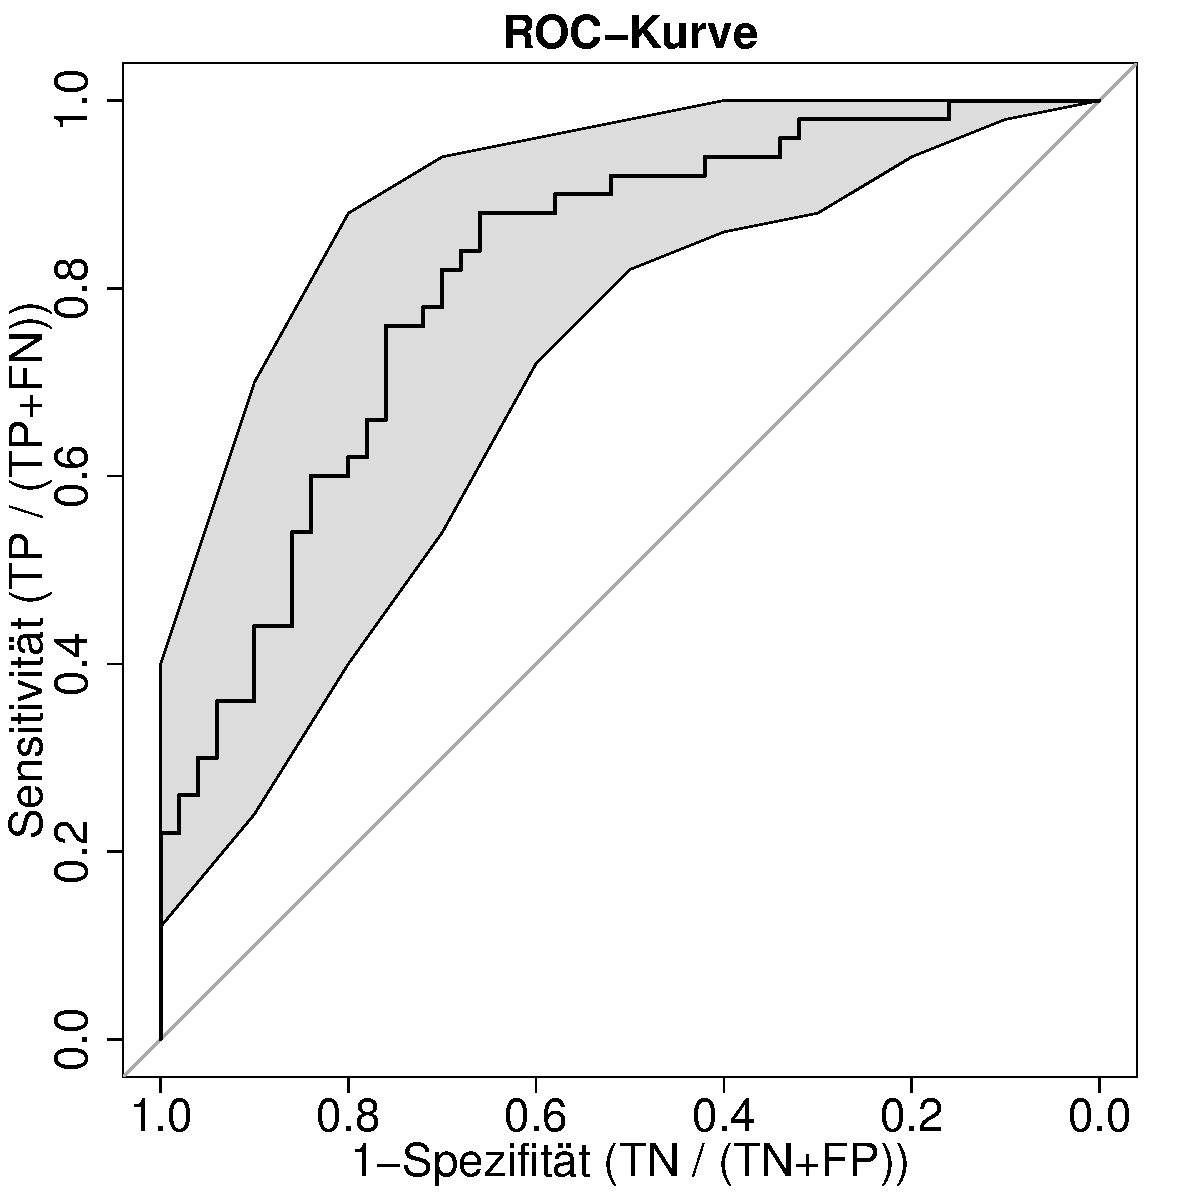
\includegraphics[width=8cm]{ROC}
\vspace*{-0.5em}
\caption{ROC-Kurve für eine dichotome Klassifikation samt Konfidenzbereich für die Sensitivität}
\label{fig:ROC}
\end{figure}

%%%%%%%%%%%%%%%%%%%%%%%%%%%%%%%%%%%%%%%%%%%%%%%%%%%%%%%%%%%%%%%%%%
%%%%%%%%%%%%%%%%%%%%%%%%%%%%%%%%%%%%%%%%%%%%%%%%%%%%%%%%%%%%%%%%%%
\section{Maße für Zusammenhang und Übereinstimmung}
%%%%%%%%%%%%%%%%%%%%%%%%%%%%%%%%%%%%%%%%%%%%%%%%%%%%%%%%%%%%%%%%%%
%%%%%%%%%%%%%%%%%%%%%%%%%%%%%%%%%%%%%%%%%%%%%%%%%%%%%%%%%%%%%%%%%%

%%%%%%%%%%%%%%%%%%%%%%%%%%%%%%%%%%%%%%%%%%%%%%%%%%%%%%%%%%%%%%%%%%
%%%%%%%%%%%%%%%%%%%%%%%%%%%%%%%%%%%%%%%%%%%%%%%%%%%%%%%%%%%%%%%%%%
\subsection[Spearmans \texorpdfstring{$\rho$}{rho} und Kendalls \texorpdfstring{$\tau$}{tau}]{Zusammenhang stetiger ordinaler Variablen: Spearmans $\bm{\rho}$ und Kendalls $\bm{\tau$}}
\label{sec:rhoTau}
%%%%%%%%%%%%%%%%%%%%%%%%%%%%%%%%%%%%%%%%%%%%%%%%%%%%%%%%%%%%%%%%%%
%%%%%%%%%%%%%%%%%%%%%%%%%%%%%%%%%%%%%%%%%%%%%%%%%%%%%%%%%%%%%%%%%%

\index{Korrelation!Rangkorrelation}
\index{Zusammenhangsmasse@Zusammenhangsmaße!Rangkorrelation}
\index{Kovarianz!Rangkovarianz}
\index{Korrelation!Spearmans $\rho$}
\index{Spearmans rho@Spearmans $\rho$}
\index[func]{cov()@\lstinline{cov()}}
\index[func]{cor()@\lstinline{cor()}}
Zur Berechnung der Kovarianz und Korrelation zweier stetiger ordinaler Variablen nach Spearman bzw.\ nach Kendall dienen die Funktionen \lstinline!cov()! und \lstinline!cor()!, für die dann das Argument \lstinline!method! auf \lstinline!"spearman"! bzw.\ auf \lstinline!"kendall"! zu setzen ist. Spearmans $\rho$ ist gleich der gewöhnlichen Pearson-Korrelation beider Variablen, nachdem ihre Werte durch die zugehörigen Ränge ersetzt wurden.\footnote{Für die polychorische und polyseriale Korrelation s.\ Abschn.\ \ref{sec:covCor}, Fußnote \ref{ftn:polycor}.}
\begin{lstlisting}
> DV1 <- c(100, 76, 56, 99, 50, 62, 36, 69, 55,  17)
> DV2 <- c(42,  74, 22, 99, 73, 44, 10, 68, 19, -34)
> cor(DV1, DV2, method="spearman")            # Spearmans rho
[1] 0.6727273

> cor(rank(DV1), rank(DV2))                   # Korrelation der Ränge
[1] 0.6727273
\end{lstlisting}

\index{Korrelation!Kendalls $\tau$}
\index{Kendalls tau@Kendalls $\tau$}
Für Kendalls $\tau_{a}$ ist die Differenz der Anzahl konkordanter Paare $n_{\text{CP}}$ und diskonkordanter Paare $n_{\text{DP}}$ von je zwei abhängigen Messwerten zu bilden und an der Gesamtzahl möglicher Paare ${n \choose 2} = \frac{n (n-1)}{2}$ zu relativieren. Sind $X$ und $Y$ die Variablen aus den abhängigen Stichproben vom Umfang $n$, ist ein Paar $\{(x_{i}, y_{i}), (x_{j}, y_{j})\}$ mit $i \neq j$ dann konkordant, wenn $x_{i}$ und $x_{j}$ dieselbe Rangordnung aufweisen wie $y_{i}$ und $y_{j}$.

Kendalls $\tau_{b}$ unterscheidet sich von $\tau_{a}$, wenn jeweils innerhalb von $X$ und $Y$ identische Werte (Bindungen) vorliegen können, wobei $n_{\text{TX}}$ die Anzahl der Bindungen in $X$ und $n_{\text{TY}}$ die Anzahl der Bindungen in $Y$ angibt. Dann relativiert $\tau_{b}$ die Differenz $n_{\text{CP}} - n_{\text{DP}}$ am geometrischen Mittel $\sqrt{(n_{\text{CP}} + n_{\text{DP}} + n_{\text{TX}}) \cdot (n_{\text{CP}} + n_{\text{DP}} + n_{\text{TY}})}$. \lstinline!cor(..., method="kendall")! berechnet bei Bindungen $\tau_{b}$.
\begin{lstlisting}
> cor(DV1, DV2, method="kendall")             # Kendalls tau-b
[1] 0.6

# Matrizen der paarweisen Rangvergleiche jeweils in X und Y
> cmpMat1 <- outer(DV1, DV1, ">")             # Vergleiche in X
> cmpMat2 <- outer(DV2, DV2, ">")             # Vergleiche in Y
> selMat  <- upper.tri(cmpMat1)     # relevant nur obere Dreiecksmatrix

# Anzahl konkordanter Paare -> Rangordnung in X und Y identisch
# setzt voraus, dass keine Bindungen existieren
> nCP <- sum((cmpMat1 == cmpMat2)[selMat])

# Anzahl diskonkordanter Paare -> Rangordnung in X und Y verschieden
> nDP    <- sum((cmpMat1 != cmpMat2)[selMat])
> N      <- length(DV1)                       # Anzahl Versuchspersonen
> nPairs <- choose(N, 2)                      # Anzahl möglicher Paare
> (tau   <- (nCP-nDP) / nPairs)               # Kendalls tau-a
[1] 0.6
\end{lstlisting}

Spearmans und Kendalls empirische Maße des Zusammenhangs lassen sich mit \lstinline!cor.test()!\index[func]{cor.test()@\lstinline{cor.test()}} inferenzstatistisch daraufhin prüfen, ob sie mit der $\text{H}_{0}$ verträglich sind, dass der theoretische Zusammenhang $0$ ist.
\begin{lstlisting}
cor.test(x=<<Vektor1>>, y=<<Vektor2>>, 
         alternative=c("two.sided", "less", "greater"),
         method=c("pearson", "kendall", "spearman"), use)
\end{lstlisting}

Die Daten beider Variablen sind als Vektoren derselben Länge über die Argumente \lstinline!x! und \lstinline!y! anzugeben. Ob die $\text{H}_{1}$ zwei- (\lstinline!"two.sided"!), links- (negativer Zusammenhang, \lstinline!"less"!) oder rechtsseitig (positiver Zusammenhang, \lstinline!"greater"!) ist, legt das Argument \lstinline!alternative! fest. Für den Test ordinaler Daten nach Spearman und Kendall ist das Argument \lstinline!method! auf \lstinline!"spearman"! bzw.\ \lstinline!"kendall"! zu setzen. Über das Argument \lstinline!use! können verschiedene Strategien zur Behandlung fehlender Werte ausgewählt werden (Abschn.\ \ref{sec:naMat}).
\begin{lstlisting}
> cor.test(DV1, DV2, method="spearman")
Spearman's rank correlation rho
data: DV1 and DV2
S = 54, p-value = 0.03938
alternative hypothesis: true rho is not equal to 0
sample estimates:
      rho
0.6727273
\end{lstlisting}

Die Ausgabe des Spearman-Tests beinhaltet den Wert der Hotelling-Pabst-Teststatistik (\lstinline!S!) nebst zugehörigem $p$-Wert (\lstinline!p-value!) und Spearmans $\rho$ (\lstinline!rho!). $S$ ergibt sich als Summe der quadrierten Differenzen zwischen den Rängen zugehöriger Messwerte in beiden Stichproben.\footnote{\label{ftn:pKendall}Die Berechnung des zugehörigen $p$-Wertes ist nur über eine intern definierte Funktion möglich, die Verteilungsfunktion der Teststatistik ist nicht direkt als R-Funktion vorhanden.}
\begin{lstlisting}
> sum((rank(DV1) - rank(DV2))^2)                  # Teststatistik S
[1] 54

> cor.test(DV1, DV2, method="kendall")            # Test nach Kendall
Kendall's rank correlation tau
data: DV1 and DV2
T = 36, p-value = 0.01667
alternative hypothesis: true tau is not equal to 0
sample estimates:
tau
0.6
\end{lstlisting}

Die Ausgabe des Kendall-Tests berichtet den Wert der Teststatistik (\lstinline!T!) gemeinsam mit dem zugehörigen $p$-Wert (\lstinline!p-value!) sowie Kendalls $\tau_{b}$ (\lstinline!tau!). $T$ ist hier als Anzahl konkordanter Paare definiert -- die Differenz der Anzahl konkordanter und diskonkordanter Paare wäre gleichermaßen geeignet, da sich beide zur festen Anzahl möglicher Paare addieren, sofern keine Bindungen vorliegen (Fußnote \ref{ftn:pKendall}).

Goodman und Kruskals $\gamma$\index{Zusammenhangsmasse@Zusammenhangsmaße!Goodman und Kruskals $\gamma$}\index{Goodman und Kruskals Gamma@Goodman und Kruskals $\gamma$} basiert ebenfalls auf der Anzahl konkordanter und diskonkordanter Paare. $\gamma$ stimmt mit Kendalls $\tau_{a}$ und $\tau_{b}$ überein, wenn keine Rangbindungen vorliegen. Bei Bindungen unterscheidet sich $\gamma$ jedoch darin, dass es die Differenz $n_{\text{CP}} - n_{\text{DP}}$ an der Summe $n_{\text{CP}} + n_{\text{DP}}$ relativiert. $\gamma$ lässt sich über \lstinline!GoodmanKruskalGamma()!\index[func]{GoodmanKruskalGamma()@\lstinline{GoodmanKruskalGamma()}} aus dem Paket \lstinline!DescTools!\index[pack]{DescTools@\lstinline{DescTools}} berechnen. Ebenfalls aus diesem Paket stammt die Funktion\index[func]{SomersDelta()@\lstinline{SomersDelta()}} \lstinline!SomersDelta()!, die\index{Zusammenhangsmasse@Zusammenhangsmaße!Somers' $d$}\index{Somers d@Somers' $d$} Somers' $d$ ausgibt -- ein weiteres Zusammenhangsmaß kategorialer Variablen, das die Anzahl konkordanter und diskonkordanter Paare berücksichtigt.

%%%%%%%%%%%%%%%%%%%%%%%%%%%%%%%%%%%%%%%%%%%%%%%%%%%%%%%%%%%%%%%%%%
%%%%%%%%%%%%%%%%%%%%%%%%%%%%%%%%%%%%%%%%%%%%%%%%%%%%%%%%%%%%%%%%%%
\subsection[Zusammenhang kategorialer Variablen]{Zusammenhang kategorialer Variablen: $\bm{\phi}$, Cramérs $\bm{V}$, Kontingenzkoeffizient}
\label{sec:assocMisc}
%%%%%%%%%%%%%%%%%%%%%%%%%%%%%%%%%%%%%%%%%%%%%%%%%%%%%%%%%%%%%%%%%%
%%%%%%%%%%%%%%%%%%%%%%%%%%%%%%%%%%%%%%%%%%%%%%%%%%%%%%%%%%%%%%%%%%

\index{Zusammenhangsmasse@Zusammenhangsmaße}
Als Maße des Zusammenhangs von zwei ungeordneten kategorialen Variablen mit $P$ bzw. mit $Q$ Kategorien dienen
\index{Zusammenhangsmasse@Zusammenhangsmaße!$\phi$-Koeffizient}
\index{Zusammenhangsmasse@Zusammenhangsmaße!Matthews-Korrelationskoeffizient}
\index{phi-Koeffizient@$\phi$-Koeffizient}
\index{Matthews-Korrelationskoeffizient}
\index{Zusammenhangsmasse@Zusammenhangsmaße!Kontingenzkoeffizient}
\index{Kontingenzkoeffizient}
\index{Zusammenhangsmasse@Zusammenhangsmaße!Cramérs $V$}
\index{Cramers V@Cramérs $V$}
\index{Zusammenhangsmasse@Zusammenhangsmaße!Tschuprows $T$}
\index{Tschuprows T@Tschuprows $T$}
\begin{itemize}
\item der $\phi$-Koeffizient (bei dichotomen Variablen gleich deren Korrelation, auch als \emph{Matthews}-Korrelationskoeffizient bezeichnet),
\item dessen Verallgemeinerung Cramérs $V$ (für dichotome Variablen identisch mit $|\phi|$),
\item der Pearson-Kontingenzkoeffizient $CC$
\item und Tschuprows $T$ (identisch zu Cramérs $V$ für quadratische Kontingenztafeln).
\end{itemize}

Diese Kennwerte basieren auf dem $\chi^{2}$-Wert der Kontingenztafel der gemeinsamen Häufigkeiten beider Variablen. Beruht die Kontingenztafel auf $n$ Beobachtungen, und ist $L = \min({P, Q})$ der kleinere Wert der Anzahl ihrer Zeilen und Spalten, gelten folgende Zusammenhänge: $n (L-1)$ ist der größtmögliche $\chi^{2}$-Wert. Weiterhin gilt $\phi = \sqrt{\frac{\chi^{2}}{n}}$, $V = \sqrt{\frac{\chi^{2}}{n (L-1)}}$, $CC = \sqrt{\frac{\chi^{2}}{n + \chi^{2}}}$ und $T = \sqrt{\frac{\phi^{2}}{\sqrt{(P-1) \cdot (Q-1)}}}$. Die Kennwerte (und einige weitere) lassen sich mit \lstinline!Assocs()!\index[func]{Assocs()@\lstinline{Assocs()}} aus dem Paket \lstinline!DescTools!\index[pack]{DescTools@\lstinline{DescTools}} ermitteln, Tschuprows $T$ mit \lstinline!TschuprowT()!\index[func]{TschuprowT()@\lstinline{TschuprowT()}} aus demselben Paket.
\begin{lstlisting}
> P    <- 2
> Q    <- 3
> DV1  <- cut(c(100, 76, 56, 99, 50, 62, 36, 69, 55,  17), breaks=P)
> DV2  <- cut(c(42,  74, 22, 99, 73, 44, 10, 68, 19, -34), breaks=Q)
> cTab <- xtabs(~ DV1 + DV2)              # Kontingenztafel
> N    <- sum(cTab)                       # Anzahl Beobachtungen
> library(DescTools)                      # für Assocs()
> Assocs(cTab)
                       estimate  lwr.ci  upr.ci
Phi Coeff.               0.5477       -       -
Contingency Coeff.       0.4804       -       -
Cramer V                 0.5477  0.0000  1.0000
Goodman Kruskal Gamma    0.7778  0.2679  1.0000
Kendall Tau-b            0.4950  0.0499  0.9401
Stuart Tau-c             0.5600  0.0423  1.0000
Somers D C|R             0.5600  0.0423  1.0000
Somers D R|C             0.4375  0.0296  0.8454
Pearson Correlation      0.5345 -0.1433  0.8710
Spearman Correlation     0.5217 -0.1607  0.8667
Lambda C|R               0.1667  0.0000  1.0000
Lambda R|C               0.4000  0.0000  1.0000
Lambda sym               0.2727  0.0000  0.9457
Uncertainty Coeff. C|R   0.1754 -0.0578  0.4087
Uncertainty Coeff. R|C   0.2671 -0.1107  0.6450
Uncertainty Coeff. sym   0.2118 -0.0766  0.5001
Mutual Information       0.2755       -       -

> TschuprowT(cTab)                        # Tschuprows T
[1] 0.4605779

# erwartete Zellhäufigkeiten
> expected <- outer(rowSums(cTab), colSums(cTab)) / N
> chisqVal <- sum((cTab-expected)^2 / expected)   # chi^2-Wert
> (phiVal  <- sqrt(chisqVal / N))         # phi-Koeffizient
[1] 0.5477226

> L        <- min(dim(cTab))              # Minimum von Zeilen, Spalten
> phisqMax <- L-1                         # maximaler phi^2-Wert
> chisqMax <- N*phisqMax                  # maximaler chi^2-Wert
> (CrV     <- sqrt(chisqVal / chisqMax))  # Cramérs V
[1] 0.5477226

> (CC <- sqrt(chisqVal / (N+chisqVal)))   # Kontingenzkoeffizient
[1] 0.4803845

> (TschT <- sqrt((chisqVal/N) / sqrt((P-1)*(Q-1))))   # Tschuprows T
[1] 0.4605779
\end{lstlisting}

Für ordinale kategoriale Variablen wird etwa von \citeA{Agresti2007} der \emph{linear-by-linear} Test auf Zusammenhang vorgeschlagen. Das Paket\index[pack]{coin@\lstinline{coin}} \lstinline!coin! stellt für seine Umsetzung\index[func]{lbl_test()@\lstinline{lbl_test()}} \lstinline!lbl_test()! bereit.

%%%%%%%%%%%%%%%%%%%%%%%%%%%%%%%%%%%%%%%%%%%%%%%%%%%%%%%%%%%%%%%%%%
%%%%%%%%%%%%%%%%%%%%%%%%%%%%%%%%%%%%%%%%%%%%%%%%%%%%%%%%%%%%%%%%%%
\subsection{Inter-Rater-Übereinstimmung}
\label{sec:irr}
%%%%%%%%%%%%%%%%%%%%%%%%%%%%%%%%%%%%%%%%%%%%%%%%%%%%%%%%%%%%%%%%%%
%%%%%%%%%%%%%%%%%%%%%%%%%%%%%%%%%%%%%%%%%%%%%%%%%%%%%%%%%%%%%%%%%%

\index{Beobachterübereinstimmung|see{Inter-Rater-Übereinstimmung}}
\index{Inter-Rater-Ubereinstimmung@Inter-Rater-Übereinstimmung}
\index{Zusammenhangsmasse@Zusammenhangsmaße!$r_{WG}$-Koeffizienten}
\index{r_WG-Koeffizienten@$r_{WG}$-Koeffizienten}
\index{Inter-Rater-Ubereinstimmung@Inter-Rater-Übereinstimmung!$r_{WG}$-Koeffizienten}
Wenn mehrere Personen (\emph{rater}) dieselben Objekte in Kategorien einordnen oder auf einer Skala bewerten, ist häufig die Inter-Rater-Übereinstimmung bzw.\ -Reliabilität als Grad der Ähnlichkeit der Urteile relevant \cite{Wirtz2002}. Hierbei lassen sich zum einen Fälle unterscheiden, bei denen entweder nur zwei oder auch mehr rater vorhanden sind. Zum anderen ist zu differenzieren, ob kontinuierliche Bewertungen oder ungeordnete bzw.\ geordnete Kategorien zum Einsatz kommen. Das im Folgenden verwendete Paket\index[pack]{DescTools@\lstinline{DescTools}} \lstinline!DescTools! bringt neben den beschriebenen noch weitere Funktionen zur Analyse der Inter-Rater-Übereinstimmung mit, etwa für Krippendorffs $\alpha$. Für den Stuart-Maxwell-Test, ob zwei rater die Kategorien einer mehrstufigen Variable mit denselben Grundwahrscheinlichkeiten verwenden, s.\ Abschn.\ \ref{sec:stuartMaxwell}.

%%%%%%%%%%%%%%%%%%%%%%%%%%%%%%%%%%%%%%%%%%%%%%%%%%%%%%%%%%%%%%%%%%
%%%%%%%%%%%%%%%%%%%%%%%%%%%%%%%%%%%%%%%%%%%%%%%%%%%%%%%%%%%%%%%%%%
\subsubsection{Prozentuale Übereinstimmung}
%%%%%%%%%%%%%%%%%%%%%%%%%%%%%%%%%%%%%%%%%%%%%%%%%%%%%%%%%%%%%%%%%%
%%%%%%%%%%%%%%%%%%%%%%%%%%%%%%%%%%%%%%%%%%%%%%%%%%%%%%%%%%%%%%%%%%

\index{Inter-Rater-Ubereinstimmung@Inter-Rater-Übereinstimmung!prozentuale Übereinstimmung}
Die relative Übereinstimmung der Urteile zweier oder mehr Personen, die dieselben Beobachtungsobjekte in mehrere Kategorien einteilen, kann mit der Funktion \lstinline!Agree()!\index[func]{Agree()@\lstinline{Agree()}} aus dem Paket \lstinline!DescTools!\index[pack]{DescTools@\lstinline{DescTools}} berechnet werden. Sie erwartet als Argument eine spaltenweise aus den Urteilen der Rater zusammengestellte Matrix. Als Beispiel diene jenes aus \citeA[p.~458~ff.]{Bortz2008a}, in dem zwei rater $100$ Beobachtungsobjekte in drei Kategorien einteilen.
\begin{lstlisting}
> categ <- c("V", "N", "P")                   # Rating-Kategorien
> lvls  <- factor(categ, levels=categ)        # Kategorien als Faktor
> rtr1  <- rep(lvls, c(60, 30, 10))           # Urteile rater 1, 2
> rtr2  <- rep(rep(lvls, nlevels(lvls)), c(53,5,2, 11,14,5, 1,6,3))
> cTab  <- xtabs(~ rtr1 + rtr2)               # Kontingenztafel
> addmargins(cTab)                            # Randsummen
           rtr2
rtr1   V   N   P  Sum
   V  53   5   2   60
   N  11  14   5   30
   P   1   6   3   10
 Sum  65  25  10  100

# relative Übereinstimmung
> library(DescTools)                          # für Agree()
> Agree(cbind(rtr1, rtr2))                    # Ausgabe gekürzt ...
[1] 0.7
\end{lstlisting}

Zur manuellen Kontrolle dient die mit \lstinline!xtabs()! ermittelte Kontingenztafel der gemeinsamen Häufigkeiten der Urteile. Übereinstimmend vergebene Kategorien stehen in der Diagonale, sofern Zeilen und Spalten dieselben Kategorien in derselben Reihenfolge umfassen.
\begin{lstlisting}
> (agree <- sum(diag(proportions(cTab))))
[1] 0.7
\end{lstlisting}

Im Anschluss soll das Beispiel um die Urteile eines dritten raters erweitert werden.
\begin{lstlisting}
> rtr3 <- rep(rep(lvls, nlevels(lvls)), c(48,8,3, 15,10,7, 3,4,2))
> Agree(cbind(rtr1, rtr2, rtr3))              # Ausgabe gekürzt ...
[1] 0.6
\end{lstlisting}

Die manuelle Kontrolle benötigt zunächst die 3D Kontingenztafel der Urteile.
\begin{lstlisting}
> cTab3 <- xtabs(~ rtr1 + rtr2 + rtr3)
> sum(diag(apply(proportions(cTab3), 3, diag)))
[1] 0.6
\end{lstlisting}

%%%%%%%%%%%%%%%%%%%%%%%%%%%%%%%%%%%%%%%%%%%%%%%%%%%%%%%%%%%%%%%%%%
%%%%%%%%%%%%%%%%%%%%%%%%%%%%%%%%%%%%%%%%%%%%%%%%%%%%%%%%%%%%%%%%%%
\subsubsection[Cohens \texorpdfstring{$\kappa$}{kappa}]{Cohens $\bm{\kappa}$}
%%%%%%%%%%%%%%%%%%%%%%%%%%%%%%%%%%%%%%%%%%%%%%%%%%%%%%%%%%%%%%%%%%
%%%%%%%%%%%%%%%%%%%%%%%%%%%%%%%%%%%%%%%%%%%%%%%%%%%%%%%%%%%%%%%%%%

\index{Inter-Rater-Ubereinstimmung@Inter-Rater-Übereinstimmung!Cohens $\kappa$}
\index{Cohens kappa@Cohens $\kappa$|see{Inter-Rater-Übereinstimmung}}
Der Grad, mit dem die Urteile zweier rater übereinstimmen, die dieselben Beobachtungsobjekte in mehrere ungeordnete Kategorien einteilen, kann mit Cohens $\kappa$-Koeffizient ausgedrückt werden. Er zielt darauf ab, den Anteil beobachteter Übereinstimmungen mit dem Anteil auch zufällig erwartbarer Übereinstimmungen in Beziehung zu setzen. Cohens $\kappa$ lässt sich mit der Funktion \lstinline!CohenKappa()!\index[func]{CohenKappa()@\lstinline{CohenKappa()}} aus dem Paket \lstinline!DescTools!\index[pack]{DescTools@\lstinline{DescTools}} berechnen, die als Argument die Kontingenztafel der Urteile beider rater erwartet. Mit \lstinline!conf.level! lässt sich zusätzlich die Breite des Konfidenzintervalls für $\kappa$ festlegen.
\begin{lstlisting}
> cTab <- xtabs(~ rtr1 + rtr2)                  # Kontingenztafel
> library(DescTools)                            # für CohenKappa()
> CohenKappa(cTab, conf.level=0.95)
    kappa     lwr.ci     upr.ci
0.4285714  0.2574917  0.5996511

# beobachteter Anteil an Übereinstimmungen (Diagonalelemente)
> fObs <- sum(diag(proportions(cTab)))

# zufällig erwartbarer Anteil an Übereinstimmungen
> fExp <- sum(rowSums(proportions(cTab)) * colSums(proportions(cTab)))
> (Ckappa <- (fObs-fExp) / (1-fExp))            # Cohens kappa
[1] 0.4285714
\end{lstlisting}

%%%%%%%%%%%%%%%%%%%%%%%%%%%%%%%%%%%%%%%%%%%%%%%%%%%%%%%%%%%%%%%%%%
%%%%%%%%%%%%%%%%%%%%%%%%%%%%%%%%%%%%%%%%%%%%%%%%%%%%%%%%%%%%%%%%%%
\subsubsection[Fleiss' \texorpdfstring{$\kappa$}{kappa}]{Fleiss' $\bm{\kappa}$}
\label{sec:kappaFleiss}
%%%%%%%%%%%%%%%%%%%%%%%%%%%%%%%%%%%%%%%%%%%%%%%%%%%%%%%%%%%%%%%%%%
%%%%%%%%%%%%%%%%%%%%%%%%%%%%%%%%%%%%%%%%%%%%%%%%%%%%%%%%%%%%%%%%%%

\index{Inter-Rater-Ubereinstimmung@Inter-Rater-Übereinstimmung!Fleiss' $\kappa$}
\index{Fleiss kappa@Fleiss' $\kappa$|see{Inter-Rater-Übereinstimmung}}
\lstinline!KappaM()!\index[func]{KappaM()@\lstinline{KappaM()}} aus dem Paket \lstinline!DescTools!\index[pack]{DescTools@\lstinline{DescTools}} ermittelt den $\kappa$-Koeffizienten nach Fleiss als Maß der Übereinstimmung von mehr als zwei ratern, die dieselben Objekte in mehrere ungeordnete Kategorien einteilen. Dafür ist die spaltenweise aus den Urteilen der rater zusammengestellte Matrix als Argument zu übergeben.

Als Beispiel diene jenes aus \citeA[p.~460~ff.]{Bortz2008a}, in dem sechs rater dieselben $30$ Begriffe einer von fünf Kategorien (a--e) zuordnen (für das Erstellen eigener Funktionen s.\ Abschn.\ \ref{sec:function}).
\begin{lstlisting}
> rtr1 <- letters[c(4,2,2,5,2, 1,3,1,1,5, 1,1,2,1,2, 3,1,1,2,1,
+                   5,2,2,1,1, 2,1,2,1,5)]
> rtr2 <- letters[c(4,2,3,5,2, 1,3,1,1,5, 4,2,2,4,2, 3,1,1,2,3,
+                   5,4,2,1,4, 2,1,2,3,5)]
> rtr3 <- letters[c(4,2,3,5,2, 3,3,3,4,5, 4,4,2,4,4, 3,1,1,4,3,
+                   5,4,4,4,4, 2,1,4,3,5)]
> rtr4 <- letters[c(4,5,3,5,4, 3,3,3,4,5, 4,4,3,4,4, 3,4,1,4,5,
+                   5,4,5,4,4, 2,1,4,3,5)]
> rtr5 <- letters[c(4,5,3,5,4, 3,5,3,4,5, 4,4,3,4,4, 3,5,1,4,5,
+                   5,4,5,4,4, 2,5,4,3,5)]
> rtr6 <- letters[c(4,5,5,5,4, 3,5,4,4,5, 4,4,3,4,5, 5,5,2,4,5,
+                   5,4,5,4,5, 4,5,4,3,5)]

# Matrix der ratings: rater in den Spalten, Objekte in den Zeilen
> rateMat <- cbind(rtr1, rtr2, rtr3, rtr4, rtr5, rtr6)
> library(DescTools)                            # für KappaM
> KappaM(rateMat, conf.level=0.95)
    kappa     lwr.ci     upr.ci
0.4302445  0.3824725  0.4780165

# manuelle Berechnung
> nRtr <- ncol(rateMat)                         # Anzahl rater
> nObs <- nrow(rateMat)                         # Anzahl Objekte

# Vektor aller Urteile
> ratings <- c(rtr1, rtr2, rtr3, rtr4, rtr5, rtr6)

# zugehöriger Faktor, welches Objekt beurteilt wurde
> obsFac <- factor(rep(1:nObs, nRtr))

# Kontingenztafel der Häufigkeiten, wie oft jedes Objekt (Zeilen)
# einer Kategorie (Spalten) zugeordnet wurde
> cTab <- xtabs(~ obsFac + ratings)

# relative Häufigkeit jeder Beurteilungskategorie
> rateTab <- proportions(xtabs(~ ratings))

# per Zufall erwartbarer Anteil an Übereinstimmungen
> fExp <- sum(rateTab^2)

# beobachtete paarweise Übereinstimmung pro Objekt
> fObsAll <- apply(cTab, 1, function(x) {
+                  sum(x*(x-1)) / (nRtr*(nRtr-1)) } )

# mittlere beobachtete paarweise Übereinstimmung
> fObs    <- mean(fObsAll)
> (Fkappa <- (fObs-fExp) / (1-fExp))            # Fleiss' kappa
[1] 0.4302445
\end{lstlisting}

%%%%%%%%%%%%%%%%%%%%%%%%%%%%%%%%%%%%%%%%%%%%%%%%%%%%%%%%%%%%%%%%%%
%%%%%%%%%%%%%%%%%%%%%%%%%%%%%%%%%%%%%%%%%%%%%%%%%%%%%%%%%%%%%%%%%%
\subsubsection[Gewichtetes Cohens \texorpdfstring{$\kappa$}{kappa}]{Gewichtetes Cohens $\bm{\kappa}$}
%%%%%%%%%%%%%%%%%%%%%%%%%%%%%%%%%%%%%%%%%%%%%%%%%%%%%%%%%%%%%%%%%%
%%%%%%%%%%%%%%%%%%%%%%%%%%%%%%%%%%%%%%%%%%%%%%%%%%%%%%%%%%%%%%%%%%

\index{Inter-Rater-Ubereinstimmung@Inter-Rater-Übereinstimmung!Cohens $\kappa$}
Liegen geordnete Kategorien vor, kann nicht nur berücksichtigt werden, ob Übereinstimmung vorliegt oder nicht, sondern auch, wie stark ggf.\ die Diskrepanz der Urteile ist. Für die Situation mit zwei ratern stehen in \lstinline!CohenKappa()!\index[func]{CohenKappa()@\lstinline{CohenKappa()}} aus dem Paket \lstinline!DescTools!\index[pack]{DescTools@\lstinline{DescTools}} mehrere Gewichtungen zur Verfügung: Wird das Argument \lstinline!weights="Equal-Spacing"! gesetzt, gilt jede Kategorie als im selben Maße unterschiedlich zu den jeweiligen Nachbarkategorien -- es soll also von gleichabständigen Kategorien ausgegangen werden.

Als Beispiel diene jenes aus \citeA[p.~484~ff.]{Bortz2008a}, in dem zwei rater die jeweils zu erwartende Einschaltquote von $100$ Fernsehsendungen einschätzen.
\begin{lstlisting}
# Beurteilungskategorien
> categ <- c("<10%", "11-20%", "21-30%", "31-40%", "41-50%", ">50%")
> lvls  <- factor(categ, levels=categ)          # Kategorien als Faktor
> tv1   <- rep(lvls, c(22, 21, 23, 16, 10, 8))  # Urteile rater 1

# Urteile rater2
> tv2 <- rep(rep(lvls, nlevels(lvls)), c(5,8,1,2,4,2, 3,5,3,5,5,0,
+            1,2,6,11,2,1,  0,1,5,4,3,3, 0,0,1,2,5,2, 0,0,1, 2,1,4))

> cTab <- xtabs(~ tv1 + tv2)                    # Kontingenztafel rater
> addmargins(cTab)                              # Randsummen
                             tv2
tv1    <10%  11-20%  21-30%  31-40%  41-50%  >50%  Sum
<10%      5       8       1       2       4     2   22
11-20%    3       5       3       5       5     0   21
21-30%    1       2       6      11       2     1   23
31-40%    0       1       5       4       3     3   16
41-50%    0       0       1       2       5     2   10
>50%      0       0       1       2       1     4    8
Sum       9      16      17      26      20    12  100

> library(DescTools)                            # für CohenKappa()
> CohenKappa(cTab, weights="Equal-Spacing", conf.level=0.95)
     kappa      lwr.ci      upr.ci
0.31566846  0.07905284  0.55228407
\end{lstlisting}

Für die manuelle Berechnung muss für jede Zelle der Kontingenztafel beider rater ein Gewicht angegeben werden, das der Ähnlichkeit der von den ratern verwendeten Kategorien entspricht. Die Gewichte bilden eine Toeplitz-Matrix mit konstanten Diagonalen, wenn sie in die Kontingenztafel eingetragen werden. Übereinstimmende Kategorien (Haupt-Diagonale) haben dabei eine Ähnlichkeit von $1$, die minimale Ähnlichkeit ist $0$. Bei gleichabständigen Kategorien sind die Gewichte dazwischen linear zu wählen (s.\ Abschn.\ \ref{sec:function} für selbst erstellte Funktionen).
\begin{lstlisting}
> P <- ncol(cTab)                               # Anzahl Kategorien

# bei Unabhängigkeit erwartete Häufigkeiten
> expected <- outer(rowSums(cTab), colSums(cTab)) / sum(cTab)

# gleichabständige Gewichtungsfaktoren für Ähnlichkeit der Kategorien
> (myWeights <- seq(0, 1, length.out=P))
[1] 0.0 0.2 0.4 0.6 0.8 1.0

# Toeplitz-Matrix der Ähnlichkeits-Gewichte
> (weightsMat <- outer(1:P, 1:P, function(x, y) {
+                      1 - ((abs(x-y)) / (P-1)) } ))
     [,1]  [,2]  [,3]  [,4]  [,5]  [,6]
[1,]  1.0   0.8   0.6   0.4   0.2   0.0
[2,]  0.8   1.0   0.8   0.6   0.4   0.2
[3,]  0.6   0.8   1.0   0.8   0.6   0.4
[4,]  0.4   0.6   0.8   1.0   0.8   0.6
[5,]  0.2   0.4   0.6   0.8   1.0   0.8
[6,]  0.0   0.2   0.4   0.6   0.8   1.0

# Summe der gewichteten beobachteten relativen Häufigkeiten
> wfObs <- sum(cTab * weightsMat) / sum(cTab)

# Summe der gewichteten erwarteten relativen Häufigkeiten
> wfExp <- sum(expected * weightsMat) / sum(cTab)

# gewichtetes Cohens kappa
> (wKappa <- (wfObs-wfExp) / (1-wfExp))
[1] 0.3156685
\end{lstlisting}

%%%%%%%%%%%%%%%%%%%%%%%%%%%%%%%%%%%%%%%%%%%%%%%%%%%%%%%%%%%%%%%%%%
%%%%%%%%%%%%%%%%%%%%%%%%%%%%%%%%%%%%%%%%%%%%%%%%%%%%%%%%%%%%%%%%%%
\subsubsection[Kendalls \texorpdfstring{$W$}{W}]{Kendalls $\bm{W}$}
%%%%%%%%%%%%%%%%%%%%%%%%%%%%%%%%%%%%%%%%%%%%%%%%%%%%%%%%%%%%%%%%%%
%%%%%%%%%%%%%%%%%%%%%%%%%%%%%%%%%%%%%%%%%%%%%%%%%%%%%%%%%%%%%%%%%%

\index{Inter-Rater-Ubereinstimmung@Inter-Rater-Übereinstimmung!Kendalls $W$}
\index{Kendalls W@Kendalls $W$|see{Inter-Rater-Übereinstimmung}}
Für stetige ordinale Urteile von mehr als zwei ratern kann Kendalls $W$ von der Funktion \lstinline!KendallW()!\index[func]{KendallW()@\lstinline{KendallW()}} aus dem Paket \lstinline!DescTools!\index[pack]{DescTools@\lstinline{DescTools}} ermittelt werden, die als Argument eine spaltenweise aus den Urteilen der rater zusammengesetzte Matrix erwartet.\footnote{Der zugehörige Signifikanztest ist äquivalent zum Friedman-Test (Abschn.\ \ref{sec:friedman}), wobei den ratern die Beobachtungsobjekte bzw.\ Blöcke entsprechen und den Objekten die unterschiedlichen Bedingungen.} Als Beispiel diene jenes aus \citeA[p.~466~ff.]{Bortz2008a}, in dem drei rater sechs Beobachtungsobjekte entsprechend der Ausprägung eines Merkmals in eine Rangreihe bringen.
\begin{lstlisting}
> rtr1    <- c(1, 6, 3, 2, 5, 4)                # Urteile rater 1
> rtr2    <- c(1, 5, 6, 2, 4, 3)                # Urteile rater 2
> rtr3    <- c(2, 3, 6, 5, 4, 1)                # Urteile rater 3
> ratings <- cbind(rtr1, rtr2, rtr3)            # Matrix der Urteile
> library(DescTools)                            # für KendallW()
> KendallW(ratings, test=TRUE)
Kendall's coefficient of concordance W
data:  ratings
Kendall chi-squared=8.5238, df=5, subjects=6, raters=3, p-value=0.1296
alternative hypothesis: W is greater 0
sample estimates:
       W
0.568254
\end{lstlisting}

Für die manuelle Berechnung wird zunächst die Matrix der Beurteiler-weisen Ränge benötigt, die im konkreten Beispiel bereits vorliegt, da Rangurteile abgegeben wurden. Bei anderen ordinalen Urteilen wäre sie aus der Matrix der ratings mit \lstinline!apply(<<ratings>>, 2, rank)! zu bilden.
\begin{lstlisting}
> rankMat  <- ratings                           # Matrix der Ränge
> nObj     <- nrow(rankMat)                     # Anzahl Objekte
> nRtr     <- ncol(rankMat)                     # Anzahl rater
> (rankSum <- rowSums(rankMat))                 # Rangsumme pro Objekt
[1] 4 14 15 9 13 8

# Summe der quadrierten Abweichungen der Rangsummen vom Erwartungswert
> (S <- sum((rankSum - (nRtr*(nObj+1) / 2))^2))
[1] 89.5

> (W <- (12 / (nRtr^2 * nObj*(nObj^2 - 1))) * S)    # Kendalls W
[1] 0.568254

> (chisqVal <- nRtr * (nObj-1) * W)                 # Teststatistik
[1] 8.52381

> (pVal <- pchisq(chisqVal, nObj-1, lower.tail=FALSE))    # p-Wert
[1] 0.1296329
\end{lstlisting}

%%%%%%%%%%%%%%%%%%%%%%%%%%%%%%%%%%%%%%%%%%%%%%%%%%%%%%%%%%%%%%%%%%
%%%%%%%%%%%%%%%%%%%%%%%%%%%%%%%%%%%%%%%%%%%%%%%%%%%%%%%%%%%%%%%%%%
\subsubsection{Intra-Klassen-Korrelation}
%%%%%%%%%%%%%%%%%%%%%%%%%%%%%%%%%%%%%%%%%%%%%%%%%%%%%%%%%%%%%%%%%%
%%%%%%%%%%%%%%%%%%%%%%%%%%%%%%%%%%%%%%%%%%%%%%%%%%%%%%%%%%%%%%%%%%

\index{Inter-Rater-Ubereinstimmung@Inter-Rater-Übereinstimmung!Intra-Klassen-Korrelation}
\index{Intra-Klassen-Korrelation|see{Inter-Rater-Übereinstimmung}}
\index{ICC|see{Inter-Rater-Übereinstimmung}}
Die Intra-Klassen-Korrelation (ICC) wird von \lstinline!ICC()!\index[func]{ICC()@\lstinline{ICC()}} aus dem Paket \lstinline!DescTools!\index[pack]{DescTools@\lstinline{DescTools}} ermittelt. Als Argument ist die Matrix der Urteile zu übergeben, wobei jede Spalte die Urteile eines raters umfasst. Die sich auf ein Objekt beziehenden Urteile befinden sich in jeweils einer Zeile.

Die ICC findet in verschiedenen Bereichen der Statistik Anwendung, u.\,a.\ eignet sie sich zur Quantifizierung der Übereinstimmung von ratern, die intervallskalierte Urteile über dieselben Objekte abgeben.\footnote{Die ICC ist kein nonparametrisches Verfahren, soll aber als Maß der Inter-Rater-Reliabilität dennoch hier aufgeführt werden.} Diese Situation lässt sich auch als Fall eines varianzanalytischen SPF-$p \cdot q$-Designs mit einem Zwischen-Gruppen-Faktor (den ratern) und einem Intra-Gruppen-Faktor (den Objekten) betrachten (Abschn.\ \ref{sec:SPFpq}). Unterschiedliche ICC-Varianten resultieren in Abhängigkeit davon, ob zum einen rater bzw.\ Objekte als feste Faktoren oder als Random-Faktoren zu betrachten sind, und ob zum anderen Einzeldaten oder bereits aggregierte Werte vorliegen.
\begin{lstlisting}
> nRtr <- 4                                 # Anzahl rater
> nObs <- 6                                 # Beobachtungen pro rater
> rtr1 <- c(9, 6, 8, 7, 10, 6)              # ratings rater 1
> rtr2 <- c(2, 1, 4, 1,  5, 2)              # " 2
> rtr3 <- c(5, 3, 6, 2,  6, 4)              # " 3
> rtr4 <- c(8, 2, 8, 6,  9, 7)              # " 4
> library(DescTools)                        # für ICC()
> ICC(cbind(rtr1, rtr2, rtr3, rtr4))
Call: ICC(x = cbind(rtr1, rtr2, rtr3, rtr4))

Intraclass correlation coefficients
                     type   ICC    F df1 df2    p lowerBound upperBound
Single_raters_abs    ICC1  0.17  1.8   5  18 0.16      -0.13       0.72
Single_random_raters ICC2  0.29 11.0   5  15 0.00       0.02       0.76
Single_fixed_raters  ICC3  0.71 11.0   5  15 0.00       0.34       0.95
Avg_raters_absolute  ICC1k 0.44  1.8   5  18 0.16      -0.88       0.91
Avg_random_raters    ICC2k 0.62 11.0   5  15 0.00       0.07       0.93
Avg_fixed_raters     ICC3k 0.91 11.0   5  15 0.00       0.68       0.99
\end{lstlisting}

Die Ausgabe nennt den Wert von sechs ICC-Varianten samt der $p$-Werte ihres jeweiligen Signifikanztests und der Grenzen des zugehörigen zweiseitigen Vertrauensintervalls. Die Varianten ICC1--ICC3 gehen davon aus, dass jeder Wert ein Einzelurteil darstellt, während die Varianten ICC1k--ICC3k für den Fall gedacht sind, dass jeder Wert seinerseits bereits ein Mittelwert mehrerer Urteile desselben raters über dasselbe Objekt ist. Welcher ICC-Wert der zu einer konkreten Untersuchung passende ist, hat der Nutzer selbst zu entscheiden, wobei eine nähere Erläuterung über \lstinline!?ICC! zu finden ist.

Für die manuelle Berechnung sind Effekt- und Residual-Quadratsummen aus zwei Varianzanalysen notwendig: zum einen aus der einfaktoriellen ANOVA (Abschn.\ \ref{sec:CRp}) mit nur den Objekten als UV, zum anderen aus der zweifaktoriellen ANOVA (Abschn.\ \ref{sec:CRFpq}) mit Objekten und ratern als Faktoren.
\begin{lstlisting}
> ratings <- c(rtr1, rtr2, rtr3, rtr4)                  # alle ratings

# zugehöriger Faktor, von welchem rater ein rating stammt
> rateFac <- factor(rep(paste("rater", 1:nRtr, sep=""), each=nObs))

# zugehöriger Faktor, zu welchem Objekt ein rating gehört
> obsFac <- factor(rep(paste("obj", 1:nObs, sep=""), times=nRtr))

# Varianzanalyse nur mit Faktor Beobachtungsobjekt
> (anObs <- anova(lm(ratings ~ obsFac)))                # ...

# zweifaktorielle Varianzanalyse: Beobachtungsobjekt und rater
> (anBoth <- anova(lm(ratings ~ obsFac + rateFac)))     # ...

# relevante mittlere Quadratsummen extrahieren
> MSobs   <-  anObs["obsFac",    "Mean Sq"] # Effekt Objekt 1fakt. ANOVA
> MSEobs  <-  anObs["Residuals", "Mean Sq"] # Residuen 1fakt. ANOVA
> MSrtr   <- anBoth["rateFac",   "Mean Sq"] # Effekt rater 2fakt. ANOVA
> MSEboth <- anBoth["Residuals", "Mean Sq"] # Residuen 2fakt. ANOVA

> (ICC1 <- (MSobs-MSEobs)   / (MSobs + (nRtr-1)*MSEobs))
[1] 0.1657418

> (ICC2 <- (MSobs-MSEboth)  / (MSobs + (nRtr-1)*MSEboth
+            + ((nRtr/nObs) * (MSrtr - MSEboth))))
[1] 0.2897638

> (ICC3 <- (MSobs-MSEboth)  / (MSobs + (nRtr-1)*MSEboth))
[1] 0.7148407

> (ICC1k <- (MSobs-MSEobs)  / (MSobs))
[1] 0.4427971

> (ICC2k <- (MSobs-MSEboth) / (MSobs + ((1/nObs) * (MSrtr-MSEboth))))
[1] 0.6200505

> (ICC3k <- (MSobs-MSEboth) /  MSobs)
[1] 0.9093155
\end{lstlisting}

%%%%%%%%%%%%%%%%%%%%%%%%%%%%%%%%%%%%%%%%%%%%%%%%%%%%%%%%%%%%%%%%%%
%%%%%%%%%%%%%%%%%%%%%%%%%%%%%%%%%%%%%%%%%%%%%%%%%%%%%%%%%%%%%%%%%%
\subsubsection{Bland-Altman Diagramm}
%%%%%%%%%%%%%%%%%%%%%%%%%%%%%%%%%%%%%%%%%%%%%%%%%%%%%%%%%%%%%%%%%%
%%%%%%%%%%%%%%%%%%%%%%%%%%%%%%%%%%%%%%%%%%%%%%%%%%%%%%%%%%%%%%%%%%

\index{Bland-Altman Diagramm}
\index{Tukey Mean Difference Plot}
Ein Bland-Altman Diagramm (auch: Tukey \emph{mean difference} Diagramm) erlaubt es, die Übereinstimmung von zwei ratern oder Messmethoden bzgl.\ einer and denselben Objekten $i$ erhobenen quantitativen Variable zu beurteilen. Dafür trägt ein Streudiagramm (Abschn.\ \ref{sec:distr2var}) die paarweise gebildeten Differenzen $d_{i}$ der Werte auf der $y$-Achse gegen ihren jeweiligen Mittelwert $m_{i}$ auf der $x$-Achse auf (Abb. \ref{fig:blandAltman}). Eine rudimentäre Version kann mit\index[func]{tmd()@\lstinline{tmd()}} \lstinline!tmd()! aus dem im Basisumfang von R enthaltenen Paket\index[pack]{lattice@\lstinline{lattice}|textbf} \lstinline!lattice! \cite{Sarkar2008} erstellt werden -- eine reichhaltigere Variante ist manuell möglich.

\begin{figure}[ht]
\centering
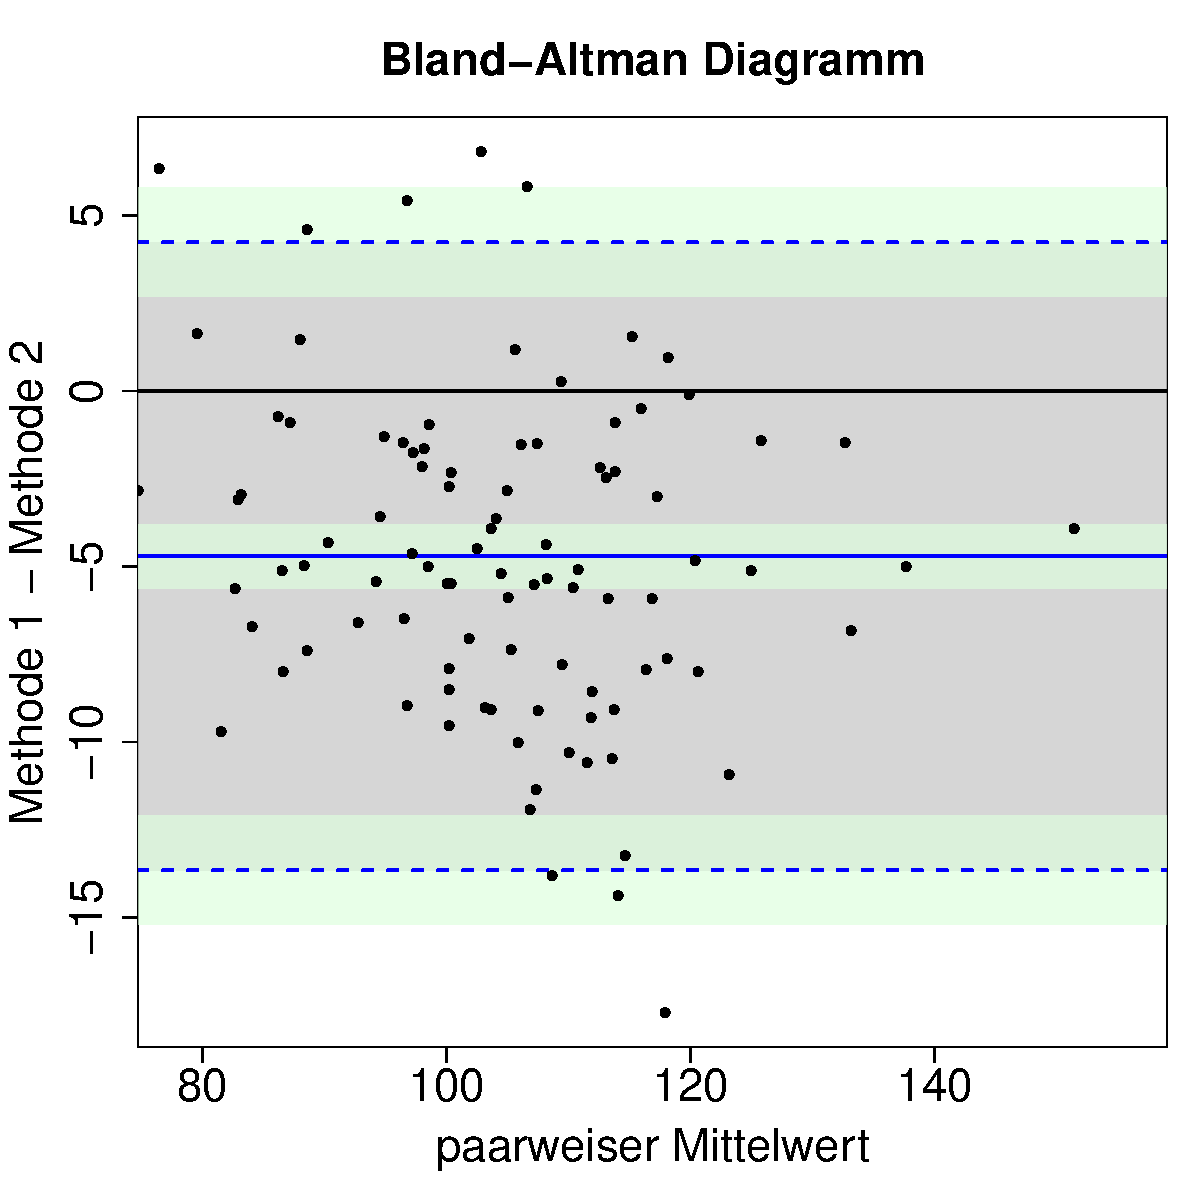
\includegraphics[width=8cm]{blandAltman}
\vspace*{-0.5em}
\caption{Bland-Altman Diagramm der paarweisen Differenzen gegen die paarweisen Mittelwerte mit \emph{bias} und \emph{limits of agreement} samt Konfidenzintervallen}
\label{fig:blandAltman}
\end{figure}

\begin{lstlisting}
> N       <- 100                        # Anzahl Messungen
> method1 <- rnorm(N, 100, 15)          # Messwerte Methode 1
> method2 <- method1 + rnorm(N, 5, 5)   # Messwerte Methode 2 (bias +5)
> m_i     <- (method1 + method2) / 2    # paarweise Mittelwerte
> d_i     <- method1 - method2          # paarweise Differenzen

# Streudiagramm paarweise Differenzen gegen paarweise Mittelwerte
> xLo <- 1.05*min(m_i)                  # x-Achse untere Grenze
> xUp <- 1.05*max(m_i)                  # x-Achse obere Grenze
> plot(m_i, d_i, pch=16, main="Bland-Altman Diagramm",
+      xlab="paarweiser Mittelwert", ylab="Methode 1 - Methode 2",
+      xlim=c(xLo, xUp), xaxs="i")
\end{lstlisting}

Eine horizontale Linie auf Höhe des Mittelwerts $\bar{d}$ der paarweisen Differenzen dient als Maß für die systematische Verzerrung (\emph{bias}). Der bias $\bar{d} \pm z_{0.975} \cdot s_{d}$ markiert den Bereich der \emph{limits of agreement}, wobei $z_{0.975}$ das 97,5\%-Quantil der Standardormalverteilung (1,96) und $s_{d}$ die Streuung der Differenzen ist. In diesem Bereich werden bei normalverteilten Differenzen 95\% der $d_{i}$ erwartet. Die limits of agreement sollten deshalb innerhalb des aus inhaltlicher Sicht noch akzeptablen Abweichungsbereichs liegen.
\begin{lstlisting}
> m_di   <- mean(d_i)                   # Mittelwert der Differenzen
> var_di <- var(d_i)                    # Varianz der Differenzen
> alpha  <- 0.05                        # Signifikanzniveau
> LoA_z  <- qnorm(1-(alpha/2), 0, 1)    # 97,5% z-Wert Standard-NV
> LoAlo  <- m_di - LoA_z*sqrt(var_di)   # LoA unten
> LoAup  <- m_di + LoA_z*sqrt(var_di)   # LoA oben

# limits of agreement-Bereich, bias und 0-bias Referenz darstellen
> rect(xLo, LoAlo, xUp, LoAup, col="#cccccccc", border=NA) # LoA Bereich
> abline(h=c(LoAlo, LoAup), col="darkgreen", lwd=2, lty=2) # LoA
> abline(h=m_di, col="blue", lwd=2)     # geschätzter bias
> abline(h=0, col="darkgray", lwd=2)    # Referenzlinie 0 = kein bias
\end{lstlisting}

Als Maß für die Präzision des berechneten bias $\bar{d}$ sowie der limits of agreement lassen sich zudem $t$-Konfidenzintervalle unter Annahme von Normalverteiltheit der Differenzen berechnen.
\begin{lstlisting}
# t-Konfidenzintervall für Erwartungswert Differenzvariable
> tCrit    <- qt(alpha/2, df=N-1, lower.tail=FALSE) # kritischer t-Wert
> mdi_CIlo <- m_di - tCrit*sqrt(var_di/N)
> mdi_CIup <- m_di + tCrit*sqrt(var_di/N)

# t-Konfidenzintervall für untere LoA-Grenze, zunächst LoA Varianz
> var_LoA    <- (var(d_i) / N) + (LoA_z^2 * var_di / (2*(N-1)))
> LoAlo_CIlo <- LoAlo - tCrit*sqrt(var_LoA)
> LoAlo_CIup <- LoAlo + tCrit*sqrt(var_LoA)

# t-Konfidenzintervall für obere LoA-Grenze
> LoAup_CIlo <- LoAup - tCrit*sqrt(var_LoA)
> LoAup_CIup <- LoAup + tCrit*sqrt(var_LoA)

# Konfidenzbereiche darstellen
> rect(xLo, LoAlo_CIlo, xUp, LoAlo_CIup, col="#ddffddaa", border=NA)
> rect(xLo, mdi_CIlo,   xUp, mdi_CIup,   col="#ddffddaa", border=NA)
> rect(xLo, LoAup_CIlo, xUp, LoAup_CIup, col="#ddffddaa", border=NA)
> points(m_i, d_i, pch=16)    # wiederhole Datenpunkte für Sichtbarkeit
\end{lstlisting}

%%%%%%%%%%%%%%%%%%%%%%%%%%%%%%%%%%%%%%%%%%%%%%%%%%%%%%%%%%%%%%%%%%
%%%%%%%%%%%%%%%%%%%%%%%%%%%%%%%%%%%%%%%%%%%%%%%%%%%%%%%%%%%%%%%%%%
\section{Tests auf gleiche Variabilität}
\label{sec:dispHom}
%%%%%%%%%%%%%%%%%%%%%%%%%%%%%%%%%%%%%%%%%%%%%%%%%%%%%%%%%%%%%%%%%%
%%%%%%%%%%%%%%%%%%%%%%%%%%%%%%%%%%%%%%%%%%%%%%%%%%%%%%%%%%%%%%%%%%

Die in Abschn.\ \ref{sec:wilcoxRankSum} und \ref{sec:kruskal} vorgestellten Tests prüfen, ob eine Variable in zwei oder mehr unabhängigen Bedingungen denselben Median besitzt. Dafür setzen sie u.\,a.\ voraus, dass die Variable in allen Bedingungen dieselbe Variabilität hat, die Verteilungen also gleich breit sind. Wird untersucht, ob die erhobenen Werte mit dieser Annahme konsistent sind, ist zu berücksichtigen, dass i.\,d.\,R.\ die $\text{H}_{0}$ den gewünschten Zustand darstellt.\footnote{Für die zugehörigen parametrischen Tests und den Fall mit mehr als zwei Gruppen s.\ Abschn.\ \ref{sec:varHom}.} Mitunter wird als informelle ad-hoc Strategie deshalb ein höher als übliches $\alpha$-Niveau in der Größenordnung von $0.2$ gewählt. Angemessenere Herangehensweisen beschreibt \citeA[Kap.~9]{Wellek2010}.

%%%%%%%%%%%%%%%%%%%%%%%%%%%%%%%%%%%%%%%%%%%%%%%%%%%%%%%%%%%%%%%%%%
%%%%%%%%%%%%%%%%%%%%%%%%%%%%%%%%%%%%%%%%%%%%%%%%%%%%%%%%%%%%%%%%%%
\subsection{Mood-Test}
\label{sec:mood}
%%%%%%%%%%%%%%%%%%%%%%%%%%%%%%%%%%%%%%%%%%%%%%%%%%%%%%%%%%%%%%%%%%
%%%%%%%%%%%%%%%%%%%%%%%%%%%%%%%%%%%%%%%%%%%%%%%%%%%%%%%%%%%%%%%%%%

\index{Mood-Test}
\index{Varianzhomogenitat@Varianzhomogenität!Mood-Test}
\index[func]{mood.test()@\lstinline{mood.test()}}
Mit dem Mood-Test lässt sich prüfen, ob die empirische Variabilität einer stetigen ordinalen Variable in zwei unabhängigen Stichproben mit der $\text{H}_{0}$ verträglich ist, dass die Variable in beiden Bedingungen dieselbe theoretische Variabilität besitzt.\footnote{\label{ftn:mood}Vorauszusetzen ist, dass die Verteilung in beiden Stichproben denselben theoretischen Median hat. Bei Zweifeln daran können die Daten zuvor gruppenweise zentriert werden, indem man von jedem Wert den Gruppenmedian abzieht.}
\begin{lstlisting}
mood.test(x=<<Vektor>>, y=<<Vektor>>,
          alternative=c("two.sided", "less", "greater"))
\end{lstlisting}

Unter \lstinline!x! und \lstinline!y! sind die Daten aus beiden Stichproben einzutragen. Alternativ zu \lstinline!x! und \lstinline!y! kann auch eine Modellformel \lstinline!<<AV>> ~ <<UV>>! eingegeben werden. Stammen die in der Modellformel verwendeten Variablen aus einem Datensatz, ist dieser unter \lstinline!data! zu nennen. Das Argument \lstinline!alternative! bezieht sich auf die Variabilität von \lstinline!x! im Vergleich zu jener von \lstinline!y!.

\begin{lstlisting}
> DV1 <- c(12, 13, 29, 30)                        # Daten Gruppe 1
> DV2 <- c(15, 17, 18, 24, 25, 26)                # Daten Gruppe 2
> Nj  <- c(length(DV1), length(DV2))              # Gruppengrößen
> DV  <- c(DV1, DV2)                              # Gesamt-Daten
> IV  <- factor(rep(1:2, Nj), labels=c("A", "B")) # welche Gruppe
> mood.test(DV ~ IV, alternative="greater")
Mood two-sample test of scale
data: DV by IV
Z = 2.6968, p-value = 0.003500
alternative hypothesis: greater
\end{lstlisting}

Die Ausgabe des Tests umfasst den Wert der $z$-transformierten Teststatistik (\lstinline!Z!), wofür Erwartungswert und Varianz einer asymptotisch gültigen Normalverteilung verwendet werden. Der $p$-Wert wird unter \lstinline!p-value! ausgegeben. Das Ergebnis lässt sich manuell prüfen, wobei auf die enge Verwandtschaft zum Wilcoxon-Rangsummen-Test hingewiesen sei (Abschn.\ \ref{sec:wilcoxRankSum}): Lediglich die Wahl der Gewichte ist hier eine andere.
\begin{lstlisting}
# Gewichte: quadrierte Differenzen der Ränge zu ihrem Mittelwert
> gX <- (rank(DV) - mean(rank(DV)))^2
> MN <- sum(gX[IV == "A"])    # Teststat.: Summe Gewichte der 1. Gruppe

# Erwartungswert und theoretische Varianz der Teststatistik
> N     <- sum(Nj)                      # Anzahl Beobachtungsobjekte
> muMN  <- (Nj[1] * (N^2 - 1)) / 12     # Erwartungswert
> varMN <- (Nj[1]*Nj[2] * (N+1) * (N^2 - 4)) / 180      # Varianz
> (MNz  <- (MN-muMN) / sqrt(varMN))     # theoretische z-Transformation
[1] 2.696799

> (pVal <- pnorm(MNz, 0, 1, lower.tail=FALSE))  # p-Wert einseitig
[1] 0.003500471
\end{lstlisting}

%%%%%%%%%%%%%%%%%%%%%%%%%%%%%%%%%%%%%%%%%%%%%%%%%%%%%%%%%%%%%%%%%%
%%%%%%%%%%%%%%%%%%%%%%%%%%%%%%%%%%%%%%%%%%%%%%%%%%%%%%%%%%%%%%%%%%
\subsection{Ansari-Bradley-Test}
%%%%%%%%%%%%%%%%%%%%%%%%%%%%%%%%%%%%%%%%%%%%%%%%%%%%%%%%%%%%%%%%%%
%%%%%%%%%%%%%%%%%%%%%%%%%%%%%%%%%%%%%%%%%%%%%%%%%%%%%%%%%%%%%%%%%%

\index{Ansari-Bradley-Test}
\index{Varianzhomogenitat@Varianzhomogenität!Ansari-Bradley-Test}
\index[func]{ansari.test()@\lstinline{ansari.test()}}
Der Ansari-Bradley-Test stellt eine Alternative zum Mood-Test dar und ist ebenfalls für den Vergleich der Variabilität von stetigen, ordinalen Daten aus zwei unabhängigen Stichproben geeignet (Fußnote \ref{ftn:mood}).
\begin{lstlisting}
ansari.test(x=<<Vektor>>, y=<<Vektor>>, exact=NULL,
            alternative=c("two.sided", "less", "greater"))
\end{lstlisting}

Unter \lstinline!x! und \lstinline!y! sind die Daten aus beiden Stichproben einzutragen. Alternativ zu \lstinline!x! und \lstinline!y! kann auch eine Modellformel \lstinline!<<AV>> ~ <<UV>>! eingegeben werden. Stammen die in der Modellformel verwendeten Variablen aus einem Datensatz, ist dieser unter \lstinline!data! zu nennen. Das Argument \lstinline!alternative! bezieht sich auf die Variabilität \lstinline!x! im Vergleich zu jener von \lstinline!y!. Für die (bei großen Stichproben u.\,U.\ etwas zeitaufwendigere) Berechnung auf Basis der exakten anstatt asymptotisch gültigen Normalverteilung ist \lstinline!exact=TRUE! zu setzen. Das folgende Beispiel verwendet die Daten aus Abschn.\ \ref{sec:mood}.
\begin{lstlisting}
> ansari.test(DV ~ IV, alternative="greater", exact=FALSE)
Ansari-Bradley test
data: DV by IV
AB = 6, p-value = 0.004687
alternative hypothesis: true ratio of scales is greater than 1
\end{lstlisting}

Die Ausgabe des Tests umfasst den Wert der Teststatistik (\lstinline!AB!) sowie den zugehörigen $p$-Wert (\lstinline!p-value!). Das Ergebnis lässt sich manuell bestätigen, wobei sich die Teststatistik lediglich in der Wahl der Gewichte von jener des Mood-Tests unterscheidet.
\begin{lstlisting}
# Gewichtung: mittlere absolute Abweichung der Ränge zu ihrem Mittel
> gX  <- mean(rank(DV)) - abs(rank(DV) - mean(rank(DV)))
> (AB <- sum(gX[IV == "A"]))  # Teststat.: Summe Gewichte der 1. Gruppe
[1] 6

# Erwartungswert und theoretische Varianz der Teststatistik
# abhängig davon, ob Gesamt-N gerade oder ungerade ist
> muABe  <- (Nj[1] * (N+2)) / 4                           # gerades N
> muABo  <- (Nj[1] * (N+1)^2) / (4*N)                     # ungerades N
> varABe <- (Nj[1]*Nj[2] * (N^2 - 4)) / (48 * (N-1))      # gerades N
> varABo <- (Nj[1]*Nj[2] * (N+1) * (3 + N^2)) / (48*N^2)  # ungerades N
> muAB   <- ifelse(N %% 2, muABo,  muABe)      # hier passender EW
> varAB  <- ifelse(N %% 2, varABo, varABe)     # hier passende Varianz
> ABz    <- (AB-muAB) / sqrt(varAB)            # theo. z-Transformation
> pnorm(ABz, 0, 1)                             # p-Wert linksseitig
[1] 0.004687384
\end{lstlisting}

%%%%%%%%%%%%%%%%%%%%%%%%%%%%%%%%%%%%%%%%%%%%%%%%%%%%%%%%%%%%%%%%%%
%%%%%%%%%%%%%%%%%%%%%%%%%%%%%%%%%%%%%%%%%%%%%%%%%%%%%%%%%%%%%%%%%%
%\newpage
\section{Tests auf Übereinstimmung von Verteilungen}
\label{sec:distrEq}
%%%%%%%%%%%%%%%%%%%%%%%%%%%%%%%%%%%%%%%%%%%%%%%%%%%%%%%%%%%%%%%%%%
%%%%%%%%%%%%%%%%%%%%%%%%%%%%%%%%%%%%%%%%%%%%%%%%%%%%%%%%%%%%%%%%%%

Die im Folgenden aufgeführten Tests lassen sich mit Werten von stetigen ordinalen (aber nicht notwendigerweise metrischen und normalverteilten) Variablen durchführen und testen Hypothesen über die Lage ihrer Verteilungen. Eine Alternative stellen die in Abschn.\ \ref{sec:permTests} vorgestellten Permutationstests dar.

%%%%%%%%%%%%%%%%%%%%%%%%%%%%%%%%%%%%%%%%%%%%%%%%%%%%%%%%%%%%%%%%%%
%%%%%%%%%%%%%%%%%%%%%%%%%%%%%%%%%%%%%%%%%%%%%%%%%%%%%%%%%%%%%%%%%%
\subsection{Kolmogorov-Smirnov-Test für zwei Stichproben}
\label{sec:ksoTest}
%%%%%%%%%%%%%%%%%%%%%%%%%%%%%%%%%%%%%%%%%%%%%%%%%%%%%%%%%%%%%%%%%%
%%%%%%%%%%%%%%%%%%%%%%%%%%%%%%%%%%%%%%%%%%%%%%%%%%%%%%%%%%%%%%%%%%

\index{Kolmogorov-Smirnov-Test!Gleichheit von Verteilungen}
Der Kolmogorov-Smirnov-Test prüft die Daten einer stetigen Variable aus zwei unabhängigen Stichproben daraufhin, ob sie mit der Nullhypothese verträglich sind, dass die Variable in beiden Bedingungen dieselbe Verteilung besitzt (für den Anpassungstest s.\ Abschn.\ \ref{sec:ksTest}). Als \emph{Omnibus}-Test prüft er gleichzeitig, ob Lage und Form beider Verteilungen übereinstimmen. Dazu wird sowohl für das Argument \lstinline!x! von \lstinline!ks.test()!\index[func]{ks.test()@\lstinline{ks.test()}} als auch für \lstinline!y! ein Datenvektor angegeben. Über das Argument \lstinline!alternative! sind ungerichtete wie gerichtete Alternativhypothesen prüfbar, wobei sich letztere darauf beziehen, ob \lstinline!y! stochastisch kleiner (\lstinline!"less"!) oder größer (\lstinline!"greater"!) als \lstinline!x! ist (Abschn.\ \ref{sec:ksTest}, Fußnote \ref{ftn:stochDom}).
\begin{lstlisting}
> DV1 <- round(rnorm(8, mean=1, sd=2), 2)         # Daten Stichprobe 1
> DV2 <- round(rnorm(8, mean=3, sd=2), 2)         # Daten Stichprobe 2
> ks.test(DV1, DV2, alternative="greater")
Two-sample Kolmogorov-Smirnov test
data: DV1 and DV2
D^+ = 0.5, p-value = 0.1353
alternative hypothesis: the CDF of x lies above that of y
\end{lstlisting}

Die Teststatistiken werden wie im Anpassungstest gebildet, wobei alle möglichen absoluten Differenzen zwischen den kumulierten relativen Häufigkeiten der Daten beider Stichproben in die Teststatistiken einfließen (Abb.\ \ref{fig:ksTwo}).
\begin{lstlisting}
> sortBoth <- sort(c(DV1, DV2))       # kombinierte sortierte Daten
> both1    <- ecdf(DV1)(sortBoth)     # kumulierte rel. Häufigkeiten 1
> both2    <- ecdf(DV2)(sortBoth)     # kumulierte rel. Häufigkeiten 2
> diff1    <- both1 - both2           # Differenzen 1
> diff2    <- c(0, both1[-length(both1)]) - both2       # Differenzen 2
> diffBoth <- c(diff1, diff2)         # kombinierte Differenzen
> (DtwoS   <- max(abs(diffBoth)))     # Teststatistik zweiseitig
[1] 0.5

> (Dless   <- abs(min(diffBoth)))     # Teststatistik "less"
[1] 0

> (Dgreat  <- abs(max(diffBoth)))     # Teststatistik "greater"
[1] 0.5

# Kontrolle über Ausgabe von ks.test()
> ks.test(DV1, DV2, alternative="less")$statistic
D^-
  0

> ks.test(DV1, DV2, alternative="two.sided")$statistic
  D
0.5

# grafische Darstellung: lege Wertebereich der x-Achse fest
> xRange <- c(min(sortBoth)-1, max(sortBoth)+1)

# zeichne kumulierte relative Häufigkeiten 1 ein
> plot(ecdf(DV1), xlim=xRange, main="Kolmogorov-Smirnov-Test für zwei
+      Stichproben", xlab=NA, col.points="blue", col.hor="blue", lwd=2)

# füge kumulierte relative Häufigkeiten 2 hinzu
> par(new=TRUE)
> plot(ecdf(DV2), xlim=xRange, main=NA, xaxt="n", xlab=NA, ylab=NA,
+      lwd=2, col.points="red", col.hor="red")

# zeichne alle möglichen Abweichungen ein
> X   <- rbind(sortBoth, sortBoth)
> Y1  <- rbind(both1, both2)
> Y2  <- rbind(c(0, both1[1:(length(both1)-1)]), both2)
> matlines(X, Y1, col="darkgray", lty=1, lwd=2)
> matlines(X, Y2, col="darkgray", lty=1, lwd=2)
> legend(x="bottomright", legend=c("kumulierte rel. Häufigkeiten 1",
+       "kumulierte rel. Häufigkeiten 2"), col=c("blue", "red"), lwd=2)
\end{lstlisting}

\begin{figure}[ht]
\centering
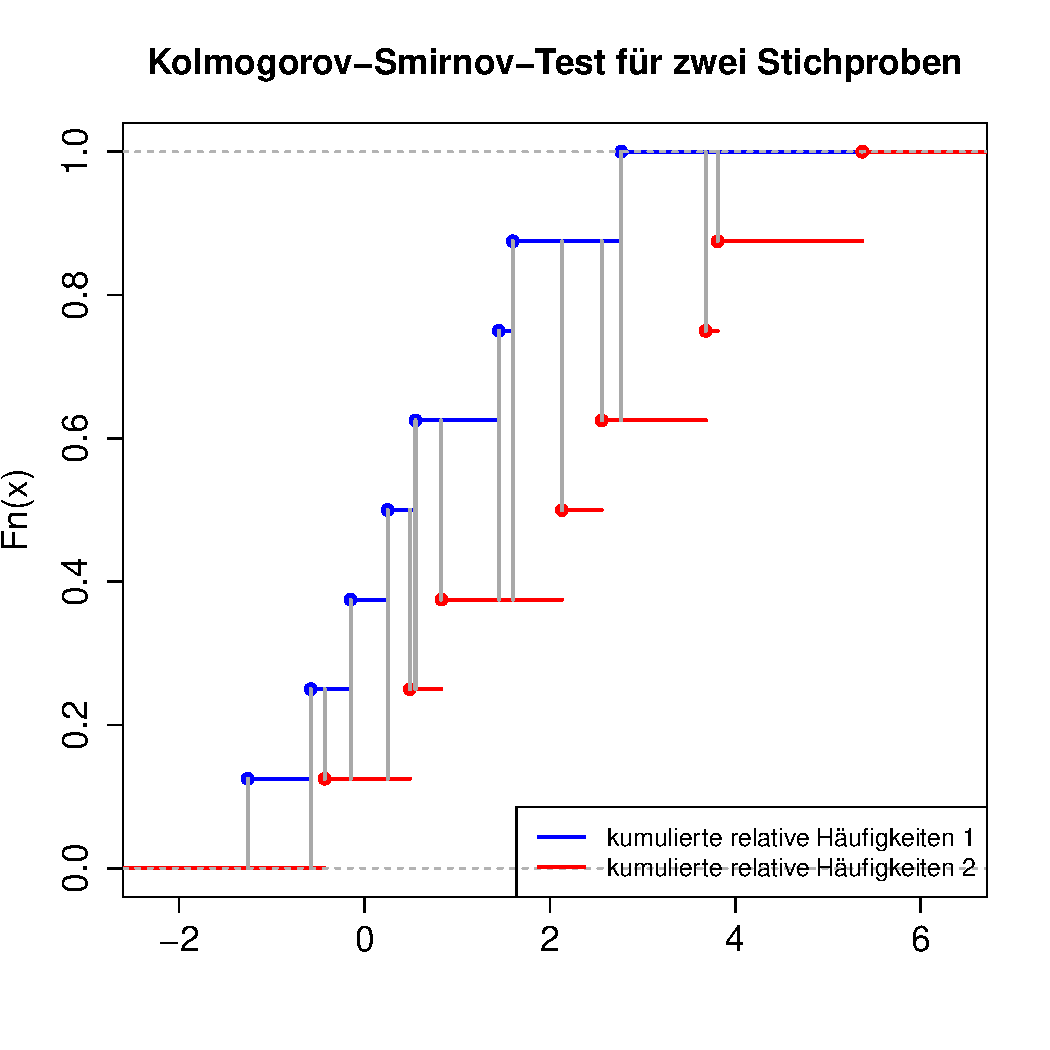
\includegraphics[width=8cm]{ksTwo}
\vspace*{-1.5em}
\caption{Kolmogorov-Smirnov-Test für zwei Stichproben: Abweichungen zwischen kumulierten relativen Häufigkeiten der Daten aus beiden Bedingungen.}
\label{fig:ksTwo}
\end{figure}

%%%%%%%%%%%%%%%%%%%%%%%%%%%%%%%%%%%%%%%%%%%%%%%%%%%%%%%%%%%%%%%%%%
%%%%%%%%%%%%%%%%%%%%%%%%%%%%%%%%%%%%%%%%%%%%%%%%%%%%%%%%%%%%%%%%%%
\subsection{Vorzeichen-Test}
\label{sec:signTest}
%%%%%%%%%%%%%%%%%%%%%%%%%%%%%%%%%%%%%%%%%%%%%%%%%%%%%%%%%%%%%%%%%%
%%%%%%%%%%%%%%%%%%%%%%%%%%%%%%%%%%%%%%%%%%%%%%%%%%%%%%%%%%%%%%%%%%

\index{Vorzeichen-Test}
\index{Binomialtest}
\index{Sign-Test|see{Vorzeichen-Test}}
Der Vorzeichen-Test für den Median ist anwendbar, wenn eine Variable eine symmetrische Verteilung unbekannter Form besitzt. Es wird die $\text{H}_{0}$ getestet, dass der Median der Verteilung gleich einem bestimmten Wert $m_{0}$ ist.\footnote{Bei Variablen mit symmetrischer Verteilung und eindeutig bestimmtem Median ist dieser gleich dem Erwartungswert, sofern letzterer existiert.} Sowohl gerichtete wie ungerichtete Alternativhypothesen sind möglich. Eine Umsetzung liefert \index[func]{SignTest()@\lstinline{SignTest()}} \lstinline!SignTest()! aus dem Paket\index[pack]{DescTools@\lstinline{DescTools}} \lstinline!DescTools!.
\begin{lstlisting}
SignTest(<<Vektor>>, mu=<<Median unter H0>>, conf.level=0.95,
         alternative=c("two.sided", "less", "greater"))
\end{lstlisting}

Neben dem Vektor der Daten ist für das Argument \lstinline!mu! der Median unter $\text{H}_{0}$ anzugeben. Die Argumente \lstinline!alternative! und \lstinline!conf.level! beziehen sich auf die Größe des Medians unter $\text{H}_{1}$ im Vergleich zu seiner Größe unter $\text{H}_{0}$ bzw.\ auf die Breite seines Vertrauensintervalls.
\begin{lstlisting}
> medH0 <- 30                               # Median unter H0
> DV    <- sample(0:100, 20, replace=TRUE)  # Daten
> library(DescTools)                        # für SignTest()
> SignTest(DV, mu=medH0)
One-sample Sign-Test
data:  DV
S = 15, number of differences = 20, p-value = 0.04139
alternative hypothesis: true median is not equal to 30
95.9 percent confidence interval:
 34 74
sample estimates:
median of the differences
                       45
\end{lstlisting}

Für die manuelle Kontrolle werden zunächst aus der Stichprobe diejenigen Werte eliminiert, die gleich $m_{0}$ sind.\footnote{Auch andere Vorgehensweisen werden diskutiert, insbesondere wenn es viele Werte gleich $m_{0}$ gibt. So können im Fall geradzahlig vieler Werte gleich $m_{0}$ die Hälfte dieser Werte als $< m_{0}$, die andere Hälfte als $> m_{0}$ codiert werden. Im Fall ungeradzahlig vieler Werte gleich $m_{0}$ wird ein Wert eliminiert und dann wie für geradzahlig viele Werte beschrieben verfahren.} Teststatistik ist die Anzahl der beobachteten Werte $> m_{0}$ -- bei intervallskalierten Daten wird also die Anzahl positiver Differenzen der Werte zu $m_{0}$ gezählt. Diese Anzahl besitzt unter $\text{H}_{0}$ eine Binomialverteilung mit der Trefferwahrscheinlichkeit $0.5$. Um den $p$-Wert der Teststatistik zu berechnen, dient \lstinline!pbinom()! für die Verteilungsfunktion der Binomialverteilung. Da die Binomialverteilung unter $\text{H}_{0}$ symmetrisch ist, kann der $p$-Wert des zweiseitigen Binomialtests als das Doppelte des einseitigen $p$-Wertes gebildet werden.
\begin{lstlisting}
> N    <- length(DV)                        # Anzahl an Beobachtungen
> DV   <- DV[DV != medH0]                   # Werte = medH0 eliminieren
> (obs <- sum(DV > medH0))                  # Teststatistik
[1] 15

# rechtsseitiger Test
> (pGreater <- pbinom(obs-1, N, 0.5, lower.tail=FALSE))
[1] 0.02069473

> (pTwoSided <- 2 * pGreater)
[1] 0.04138947
\end{lstlisting}

Der Vorzeichentest lässt sich ebenso auf Daten einer Variable aus zwei abhängigen Stichproben anwenden, deren zugehörige Verteilungen darauf getestet werden sollen, ob ihre Lageparameter identisch sind. Hierfür ist ebenfalls \lstinline!SignTest()! geeignet, wobei die Funktion intern die paarweisen Differenzen bildet und wie beschrieben mit $m_{0}=0$ testet.

%%%%%%%%%%%%%%%%%%%%%%%%%%%%%%%%%%%%%%%%%%%%%%%%%%%%%%%%%%%%%%%%%%
%%%%%%%%%%%%%%%%%%%%%%%%%%%%%%%%%%%%%%%%%%%%%%%%%%%%%%%%%%%%%%%%%%
\subsection{Wilcoxon-Vorzeichen-Rang-Test für eine Stichprobe}
\label{sec:wilcoxSignRank}
%%%%%%%%%%%%%%%%%%%%%%%%%%%%%%%%%%%%%%%%%%%%%%%%%%%%%%%%%%%%%%%%%%
%%%%%%%%%%%%%%%%%%%%%%%%%%%%%%%%%%%%%%%%%%%%%%%%%%%%%%%%%%%%%%%%%%

\index{Wilcoxon-Test!Vorzeichen-Rang-Test}
Der Wilcoxon-Vorzeichen-Rang-Test prüft, ob die in einer Stichprobe ermittelten Werte einer Variable mit symmetrischer Verteilung mit der $\text{H}_{0}$ verträglich sind, dass der Median der Verteilung gleich einem bestimmten Wert $m_{0}$ ist. Anders als beim $t$-Test für eine Stichprobe (Abschn.\ \ref{sec:tOne}) wird nicht vorausgesetzt, dass die Variable normalverteilt ist. Im Vergleich zum Vorzeichen-Test für den Median wird neben der Anzahl der Werte $> m_{0}$ auch das Ausmaß ihrer Differenz zu $m_{0}$\index[func]{wilcox.test()@\lstinline{wilcox.test()}|textbf} berücksichtigt.
\begin{lstlisting}
wilcox.test(x=<<Vektor>>, alternative=c("two.sided", "less", "greater"),
            mu=0, conf.int=FALSE)
\end{lstlisting}

Unter \lstinline!x! ist der Datenvektor einzutragen. Alternativ zu \lstinline!x! kann auch eine Modellformel \lstinline!<<AV>> ~ 1! angegeben werden. Stammt dabei die Variable \lstinline!<<AV>>! aus einem Datensatz, ist dieser unter \lstinline!data! zu nennen. Mit \lstinline!alternative! wird festgelegt, ob die $\text{H}_{1}$ bzgl.\ des Vergleichs mit dem unter $\text{H}_{0}$ angenommenen Median \lstinline!mu! gerichtet oder ungerichtet ist. \lstinline!"less"! und \lstinline!"greater"! beziehen sich dabei auf die Reihenfolge Median unter $\text{H}_{1}$ \lstinline!"less"! bzw.\ \lstinline!"greater"! $m_{0}$. Um ein Konfidenzintervall für den Median zu erhalten, ist \lstinline!conf.int=TRUE! zu setzen.

Als Beispiel diene jenes aus \citeA[p.~90~ff.]{Buning1994}: An Studenten einer Fachrichtung sei der IQ-Wert erhoben worden. Diese Werte sollen daraufhin geprüft werden, ob sie mit der $\text{H}_{0}$ verträglich sind, dass der theoretische Median $110$ beträgt. Unter $\text{H}_{1}$ sei der Median größer.
\begin{lstlisting}
> IQ    <- c(99, 131, 118, 112, 128, 136, 120, 107, 134, 122)
> medH0 <- 110                           # Median unter H0
> wilcox.test(IQ, alternative="greater", mu=medH0, conf.int=TRUE)
Wilcoxon signed rank test
data: IQ
V = 48, p-value = 0.01855
alternative hypothesis: true location is greater than 110
95 percent confidence interval:
113.5  Inf
sample estimates:
(pseudo)median
121

# alternativer Aufruf mit Modellformel für Variable aus Datensatz
> IQdat <- data.frame(IQ=IQ)
> wilcox.test(IQ ~ 1, alternative="greater", data=IQdat,
+             mu=medH0, conf.int=TRUE)   # ...
\end{lstlisting}

Die Ausgabe liefert die Teststatistik (\lstinline!V!) und den $p$-Wert (\lstinline!p-value!). Das Ergebnis lässt sich manuell nachvollziehen. Die diskret verteilte Teststatistik berechnet sich dabei als Summe der Ränge der absoluten Differenzen zu $m_{0}$, wobei nur die Ränge von Werten aufsummiert werden, die $> m_{0}$ sind. Um den $p$-Wert der Teststatistik zu erhalten, dient \lstinline!psignrank()! als Verteilungsfunktion der Teststatistik (Abschn.\ \ref{sec:distrFunc}, Fußnote \ref{ftn:distrFuncDiscr}). Wurde \lstinline!conf.int=TRUE! gesetzt, enthält die Ausgabe neben dem Konfidenzintervall für den Pseudo-Median \index{Pseudo-Median}\index{Median!Pseudo-Median} unter \lstinline!(pseudo)median! den zugehörigen\index{Hodges-Lehmann-Schatzer@Hodges-Lehmann-Schätzer} Hodges-Lehmann-Schätzer (Abschn.\ \ref{sec:meanRob}).
\begin{lstlisting}
> (diffIQ <- IQ-medH0)            # Differenzen zum Median unter H0
[1] -11 21 8 2 18 26 10 -3 24 12

> (idx <- diffIQ > 0)             # Wert > Median unter H0?
[1] FALSE TRUE TRUE TRUE TRUE TRUE TRUE FALSE TRUE TRUE

# Ränge der absoluten Differenzen zum Median unter H0
> (rankDiff <- rank(abs(diffIQ)))
[1] 5 8 3 1 7 10 4 2 9 6

# Teststatistik: Summe über die Ränge von Werten > Median unter H0
> (V <- sum(rankDiff[idx]))
[1] 48

# p-Wert einseitig
> (pVal <- psignrank(V-1, length(IQ), lower.tail=FALSE))
[1] 0.01855469

# Hodges-Lehmann-Schätzer: Median der Mittelwerte aller Wertepaare
> pairM  <- outer(IQ, IQ, FUN="+") / 2        # Mittelwerte aller Paare
> (HLloc <- median(pairM[lower.tri(pairM, diag=TRUE)]))  # deren Median
[1] 121
\end{lstlisting}

%%%%%%%%%%%%%%%%%%%%%%%%%%%%%%%%%%%%%%%%%%%%%%%%%%%%%%%%%%%%%%%%%%
%%%%%%%%%%%%%%%%%%%%%%%%%%%%%%%%%%%%%%%%%%%%%%%%%%%%%%%%%%%%%%%%%%
\subsection[Wilcoxon-Rangsummen-Test / Mann-Whitney-\texorpdfstring{$U$}{U}-Test]{Wilcoxon-Rangsummen-Test / Mann-Whitney-$\bm{U}$-Test für zwei unabhängige Stichproben}
\label{sec:wilcoxRankSum}
%%%%%%%%%%%%%%%%%%%%%%%%%%%%%%%%%%%%%%%%%%%%%%%%%%%%%%%%%%%%%%%%%%
%%%%%%%%%%%%%%%%%%%%%%%%%%%%%%%%%%%%%%%%%%%%%%%%%%%%%%%%%%%%%%%%%%

\index{Wilcoxon-Test!Rangsummen-Test}
Im Wilcoxon-Rangsummen-Test für unabhängige Stichproben werden die in zwei Stichproben ermittelten Werte einer stetigen ordinalen Variable daraufhin miteinander verglichen, ob sie mit der $\text{H}_{0}$ verträglich sind, dass die Verteilungen der Variable in den zugehörigen Bedingungen identisch sind. Anders als im analogen $t$-Test (Abschn.\ \ref{sec:tTwoInd}) wird nicht vorausgesetzt, dass die Variable in den Gruppen normalverteilt ist. Gefordert wird jedoch, dass die Verteilungen in ihrer Form in beiden Bedingungen übereinstimmen, d.\,h.\ lediglich ggf.\ horizontal verschobene Versionen voneinander sind. Es kann sowohl gegen eine ungerichtete wie gerichtete $\text{H}_{1}$ getestet werden, die sich auf den Lageparameter der Verteilungen (etwa den Median)\index[func]{wilcox.test()@\lstinline{wilcox.test()}} bezieht.\footnote{Ohne Annahme gleicher Verteilungsform beziehen sich Null- und Alternativhypothese auf die Wahrscheinlichkeit dafür, dass eine zufällige Beobachtung aus der ersten Gruppe größer bzw.\ kleiner als eine zufällig gezogene Beobachtung aus der zweiten Gruppe ist.}
\begin{lstlisting}
wilcox.test(x=<<Vektor>>, y=<<Vektor>>, paired=FALSE, conf.int=FALSE,
            alternative=c("two.sided", "less", "greater"))
\end{lstlisting}

Unter \lstinline!x! sind die Daten der ersten Stichprobe einzutragen, unter \lstinline!y! entsprechend die der zweiten. Alternativ zu \lstinline!x! und \lstinline!y! kann auch eine Modellformel \lstinline!<<AV>> ~ <<UV>>! angegeben werden. Dabei ist \lstinline!<<UV>>! ein Gruppierungsfaktor derselben Länge wie \lstinline!<<AV>>! und gibt für jede Beobachtung in \lstinline!<<AV>>! die Gruppenzugehörigkeit an. Geschieht dies mit Variablen, die aus einem Datensatz stammen, muss dieser unter \lstinline!data! eingetragen werden. Mit \lstinline!alternative! wird festgelegt, ob die $\text{H}_{1}$ gerichtet oder ungerichtet ist. \lstinline!"less"! und \lstinline!"greater"! beziehen sich dabei auf den Lageparameter in der Reihenfolge \lstinline!x! \lstinline!"less"! bzw.\ \lstinline!"greater"! \lstinline!y!. Das Argument \lstinline!paired=FALSE! bestimmt, dass es sich um unabhängige Stichproben handelt. Um ein Konfidenzintervall für die Differenz der Lageparameter zu erhalten, ist \lstinline!conf.int=TRUE! zu setzen.

Als Beispiel diene jenes aus \citeA[p.~201~ff.]{Bortz2008a}: Es wird vermutet, dass sich durch die Einnahme eines Medikaments die Reaktionszeit im Vergleich zu einer Kontrollgruppe verkürzen lässt.
\begin{lstlisting}
> rtCtrl <- c(85,106,118,81,138,90,112,119,107,95,88,103)
> rtDrug <- c(96,105,104,108,86,84,99,101,78,124,121,97,129,87,109)
> Nj     <- c(length(rtCtrl), length(rtDrug))   # Gruppengrößen

# Faktor der Gruppenzugehörigkeiten
> IV    <- factor(rep(1:2, Nj), labels=c("control", "drug"))
> rtAll <- c(rtCtrl, rtDrug)                    # Gesamtstichprobe
> wilcox.test(rtAll ~ IV, alternative="greater", conf.int=TRUE)
Wilcoxon rank sum test
data: rtAll by IV
W = 94, p-value = 0.4333
alternative hypothesis: true location shift is greater than 0
95 percent confidence interval:
-11 Inf
sample estimates:
difference in location
                     2
\end{lstlisting}

Die Ausgabe nennt den Wert der Teststatistik (\lstinline!W!) gefolgt vom $p$-Wert (\lstinline!p-value!). Das Ergebnis lässt sich manuell nachvollziehen. Dazu muss für die Daten der ersten Stichprobe die Summe ihrer Ränge in der Gesamtstichprobe ermittelt werden. Die diskret verteilte Teststatistik ergibt sich, indem von dieser Rangsumme ihr theoretisches Minimum $\sum_{i=1}^{n_{1}} i = \frac{n_{1} (n_{1} + 1)}{2}$ abgezogen wird. Um den $p$-Wert zu erhalten, dient \lstinline!pwilcox()! als Verteilungsfunktion der Teststatistik (Abschn.\ \ref{sec:distrFunc}, Fußnote \ref{ftn:distrFuncDiscr}). Wurde \lstinline!conf.int=TRUE! gesetzt, enthält die Ausgabe neben dem Konfidenzintervall für die Differenz der Lageparameter unter \lstinline!difference in location! den zugehörigen\index{Hodges-Lehmann-Schatzer@Hodges-Lehmann-Schätzer} Hodges-Lehmann-Schätzer (Abschn.\ \ref{sec:meanRob}).
\begin{lstlisting}
> gX <- rank(rtAll)                       # Gewichte = Ränge
> (W <- sum(gX[IV == "control"]) - sum(1:Nj[1]))    # Teststatistik
[1] 94

# p-Wert einseitig
> (pVal <- pwilcox(W-1, Nj[1], Nj[2], lower.tail=FALSE))
[1] 0.433342

# Hodges-Lehmann-Schätzer der Differenz der Lageparameter
> pairD <- outer(rtCtrl, rtDrug, "-")     # alle paarweisen Differenzen
> (HLdl <- median(pairD))                 # deren Median
[1] 2
\end{lstlisting}

\index{alpha-Adjustierung@$\alpha$-Adjustierung}
\index[func]{pairwise.wilcox.test()@\lstinline{pairwise.wilcox.test()}}
Die Funktion \lstinline!pairwise.wilcox.test()! dient dazu, simultan alle paarweisen Vergleiche zwischen jeweils zwei von insgesamt mehreren Gruppen mit dem Wilcoxon-Rangsummen-Test durchzuführen. Sie bietet mit dem Argument \lstinline!p.adjust.method! verschiedene Möglichkeiten zur Adjustierung des $\alpha$-Niveaus.

\index{Mann-Whitney-U-Test@Mann-Whitney-$U$-Test}
Der Mann-Whitney-$U$-Test zählt für jeden Wert der ersten Stichprobe, wie viele Werte der zweiten Stichprobe kleiner als er sind. Die Teststatistik $U$ ist die Summe dieser Häufigkeiten und führt zum selben Wert wie die oben definierte Teststatistik des Wilcoxon-Tests, besitzt also auch dieselbe Verteilung.
\begin{lstlisting}
> (U <- sum(outer(rtCtrl, rtDrug, ">=")))
[1] 94
\end{lstlisting}

%%%%%%%%%%%%%%%%%%%%%%%%%%%%%%%%%%%%%%%%%%%%%%%%%%%%%%%%%%%%%%%%%%
%%%%%%%%%%%%%%%%%%%%%%%%%%%%%%%%%%%%%%%%%%%%%%%%%%%%%%%%%%%%%%%%%%
\subsection{Wilcoxon-Test für zwei abhängige Stichproben}
\label{sec:wilcox_two_dep}
%%%%%%%%%%%%%%%%%%%%%%%%%%%%%%%%%%%%%%%%%%%%%%%%%%%%%%%%%%%%%%%%%%
%%%%%%%%%%%%%%%%%%%%%%%%%%%%%%%%%%%%%%%%%%%%%%%%%%%%%%%%%%%%%%%%%%

\index{Wilcoxon-Test!abhängige Stichproben}
Der Wilcoxon-Test für zwei abhängige Stichproben wird wie jener für unabhängige Stichproben durchgeführt, jedoch ist hier das Argument \lstinline!paired=TRUE! von \lstinline!wilcox.test()!\index[func]{wilcox.test()@\lstinline{wilcox.test()}} zu verwenden. Der Test setzt voraus, dass sich die in \lstinline!x! und \lstinline!y! angegebenen Daten einander paarweise zuordnen lassen, weshalb \lstinline!x! und \lstinline!y! dieselbe Länge besitzen müssen. Alternativ kann auch eine Modellformel \lstinline!Pair(x, y) ~ 1! verwendet werden, wobei dann das Argument \lstinline!paired=TRUE! entfällt. Sind \lstinline!x! und \lstinline!y! aus der Modellformel Teil eines Datensatzes, ist dieser unter \lstinline!data! zu nennen.

Bei im Long-Format vorliegenden Daten kann analog zum Test für zwei unabhängige Stichproben eine Modellformel \lstinline!<<AV>> ~ <<UV>>! angegeben werden -- ggf.\ zusammen mit einem Datensatz \lstinline!data!, aus dem die Variablen stammen. Die Daten in \lstinline!<<AV>>! müssen so geordnet sein, dass innerhalb jeder von \lstinline!<<UV>>! definierten Gruppe dieselbe Reihenfolge von Beobachtungsobjekten vorliegt, um die paarweise Zuordnung sicherzustellen. Zudem dürfen keine fehlenden Werte vorhanden sein.

Nach Bildung der paarweisen Differenzen einander zugeordneter Werte wird im Wilcoxon-Vorzeichen-Rang-Test für eine Stichprobe die $\text{H}_{0}$ getestet, dass der theoretische Median der Differenzwerte gleich $0$ ist.
\begin{lstlisting}
> N      <- 20                                # Stichprobengröße
> DVpre  <- rnorm(N, mean=90,  sd=15)         # Daten prä
> DVpost <- rnorm(N, mean=100, sd=15)         # Daten post
> DV     <- c(DVpre, DVpost)                  # Gesamt-Daten

# Faktor, der jedem Wert von DV Messzeitpunkt zuordnet
# dabei Kontrolle der Reihenfolge der Faktorstufen: pre vor post
> IV <- factor(rep(0:1, each=N), labels=c("pre", "post"))
> wilcox.test(DV ~ IV, alternative="less", paired=TRUE)
Wilcoxon signed rank test
data:  DV by IV
V = 28, p-value = 0.001356
alternative hypothesis: true location shift is less than 0

# äquivalent: 1-Stichproben Test der Differenzvariable
> DVdiff <- DVpre - DVpost                    # Differenzvariable
> wilcox.test(DVdiff, alternative="less")     # ...
\end{lstlisting}

%%%%%%%%%%%%%%%%%%%%%%%%%%%%%%%%%%%%%%%%%%%%%%%%%%%%%%%%%%%%%%%%%%
%%%%%%%%%%%%%%%%%%%%%%%%%%%%%%%%%%%%%%%%%%%%%%%%%%%%%%%%%%%%%%%%%%
\subsection[Kruskal-Wallis-\texorpdfstring{$H$}{H}-Test für unabhängige Stichproben]{Kruskal-Wallis-$\bm{H}$-Test für unabhängige Stichproben}
\label{sec:kruskal}
%%%%%%%%%%%%%%%%%%%%%%%%%%%%%%%%%%%%%%%%%%%%%%%%%%%%%%%%%%%%%%%%%%
%%%%%%%%%%%%%%%%%%%%%%%%%%%%%%%%%%%%%%%%%%%%%%%%%%%%%%%%%%%%%%%%%%

\index{Kruskal-Wallist-H-Test@Kruskal-Wallis-$H$-Test}
Der Kruskal-Wallis-$H$-Test verallgemeinert die Fragestellung eines Wilcoxon-Tests auf Situationen, in denen Werte einer Variable in mehr als zwei unabhängigen Stichproben ermittelt wurden. Unter $\text{H}_{0}$ sind die Verteilungen der Variable in den zugehörigen Bedingungen identisch. Die unspezifische $\text{H}_{1}$ besagt, dass sich mindestens zwei Lageparameter unterscheiden. Anders als in der einfaktoriellen Varianzanalyse (Abschn.\ \ref{sec:CRp}) wird nicht vorausgesetzt, dass die Variable in den Bedingungen normalverteilt ist. Gefordert wird jedoch, dass die Form der Verteilungen in allen Bedingungen übereinstimmt, die Verteilungen also lediglich ggf.\ horizontal verschobene Versionen voneinander\index[func]{kruskal.test()@\lstinline{kruskal.test()}} darstellen.
\begin{lstlisting}
kruskal.test(formula=<<Modellformel>>, data=<<Datensatz>>)
\end{lstlisting}

Unter \lstinline!formula! sind Daten und Gruppierungsvariable als Modellformel \lstinline!<<AV>> ~ <<UV>>! zu nennen, wobei \lstinline!<<UV>>! ein Gruppierungsfaktor derselben Länge wie \lstinline!<<AV>>! ist und für jede Beobachtung in \lstinline!<<AV>>! die Gruppenzugehörigkeit angibt. Geschieht dies mit Variablen, die aus einem Datensatz stammen, muss dieser unter \lstinline!data! eingetragen werden.

Als Beispiel diene jenes aus \citeA[p.~183~ff.]{Buning1994}: Es wird vermutet, dass der IQ-Wert in vier Studiengängen einen unterschiedlichen Erwartungswert besitzt.
\begin{lstlisting}
# IQ-Werte in den einzelnen Studiengängen
> IQ1 <- c(99, 131, 118, 112, 128, 136, 120, 107, 134, 122)
> IQ2 <- c(134, 103, 127, 121, 139, 114, 121, 132)
> IQ3 <- c(120, 133, 110, 141, 118, 124, 111, 138, 120)
> IQ4 <- c(117, 125, 140, 109, 128, 137, 110, 138, 127, 141, 119, 148)
> DV  <- c(IQ1, IQ2, IQ3, IQ4)                    # kombinierte Daten

# Stichprobengrößen
> Nj <- c(length(IQ1), length(IQ2), length(IQ3), length(IQ4))
> N  <- sum(Nj)                                   # Gesamt-N

# Faktor der Gruppenzugehörigkeiten
> IV   <- factor(rep(1:4, Nj), labels=c("I", "II", "III", "IV"))
> KWdf <- data.frame(IV, DV)                      # Datensatz
> kruskal.test(DV ~ IV, data=KWdf)
Kruskal-Wallis rank sum test
data: DV by IV
Kruskal-Wallis chi-squared = 1.7574, df = 3, p-value = 0.6242
\end{lstlisting}

Die Ausgabe nennt den Wert der asymptotisch $\chi^{2}$-verteilten $H$-Teststatistik gefolgt von den Freiheitsgraden (\lstinline!df!) und dem $p$-Wert (\lstinline!p-value!). Das Ergebnis lässt sich manuell nachvollziehen, wobei das zentrale Element der Teststatistik das Quadrat der pro Gruppe gebildeten Summe der Ränge in der Gesamtstichprobe ist, das jeweils an der zugehörigen Gruppengröße relativiert wird.\footnote{Im gewählten Beispiel sind die Ränge nicht eindeutig, es treten also Bindungen auf. Für diesen Fall gibt \lstinline!rank()! in der Voreinstellung mittlere Ränge aus, was vom Vorgehen in \lstinline!kruskal.test()! abweicht. Die manuell berechnete Teststatistik und der $p$-Wert stimmen deshalb nicht exakt mit jenen aus \lstinline!kruskal.test()! überein.}
\begin{lstlisting}
> (rankSumI <- tapply(rank(DV), IV, sum))       # Rangsumme pro Gruppe
    I     II    III     IV
168.5  160.0  173.0  278.5

> (H <- (12 / (N*(N+1))) * sum(rankSumI^2/Nj) - 3*(N+1))   # Teststat.
[1] 1.75531

> (pVal <- pchisq(H, nlevels(IV)-1, lower.tail=FALSE))     # p-Wert
[1] 0.624708
\end{lstlisting}

\index{Jonckheere-Terpstra-Test}
Für den Jonckheere-Terpstra-Trend-Test für geordnete Gruppen s.\ \index[func]{JonckheereTerpstraTest()@\lstinline{JonckheereTerpstraTest()}} \lstinline!JonckheereTerpstraTest()! aus dem Paket \index[pack]{DescTools@\lstinline{DescTools}} \lstinline!DescTools!. Tests nach Dunn bzw.\ Conover-Iman sind post-hoc Paarvergleiche auf Basis von Rangsummen, deren Testlogik zum Kruskal-Wallis-$H$-Test passen. Sie lassen sich mit \index[func]{DunnTest()@\lstinline{DunnTest()}} \lstinline!DunnTest()! bzw.\ \index[func]{ConoverTest()@\lstinline{ConoverTest()}} \lstinline!ConoverTest()! ebenfalls aus dem Paket \index[pack]{DescTools@\lstinline{DescTools}} \lstinline!DescTools! durchführen.

%%%%%%%%%%%%%%%%%%%%%%%%%%%%%%%%%%%%%%%%%%%%%%%%%%%%%%%%%%%%%%%%%%
%%%%%%%%%%%%%%%%%%%%%%%%%%%%%%%%%%%%%%%%%%%%%%%%%%%%%%%%%%%%%%%%%%
\subsection{Friedman-Rangsummen-Test für abhängige Stichproben}
\label{sec:friedman}
%%%%%%%%%%%%%%%%%%%%%%%%%%%%%%%%%%%%%%%%%%%%%%%%%%%%%%%%%%%%%%%%%%
%%%%%%%%%%%%%%%%%%%%%%%%%%%%%%%%%%%%%%%%%%%%%%%%%%%%%%%%%%%%%%%%%%

\index{Friedman-Test}
Der Rangsummen-Test nach Friedman dient der Analyse von Daten einer Variable, die in $p$ abhängigen Stichproben erhoben wurde. Jede Menge von $p$ abhängigen Beobachtungen (eine aus jeder Bedingung) wird dabei als Block bezeichnet und stammt entweder vom selben Beobachtungsobjekt (Messwiederholung) oder von mehreren homogenen (gematchten) Beobachtungsobjekten. Wie im Kruskal-Wallis-$H$-Test wird die $\text{H}_{0}$ geprüft, dass die Verteilung der Variable in allen Bedingungen identisch ist. Die unspezifische $\text{H}_{1}$ besagt, dass sich mindestens zwei Lageparameter unterscheiden. Anders als in der einfaktoriellen Varianzanalyse für abhängige Gruppen (Abschn.\ \ref{sec:RBp}) wird nicht vorausgesetzt, dass die blockweise als Vektor zusammengefasste Variable gemeinsam normalverteilt\index[func]{friedman.test()@\lstinline{friedman.test()}} ist.
\begin{lstlisting}
friedman.test(y=<<Daten>>, groups=<<Faktor>>, blocks=<<Faktor>>)
\end{lstlisting}

Die Daten müssen im Long-Format vorliegen (Abschn.\ \ref{sec:reshape}): Unter \lstinline!y! ist der Vektor aller Daten anzugeben. Als zweites Argument wird für \lstinline!groups! ein Faktor derselben Länge wie \lstinline!y! übergeben, der die Gruppenzugehörigkeit jeder Beobachtung in \lstinline!y! codiert. \lstinline!blocks! ist ebenfalls ein Faktor derselben Länge wie \lstinline!y! und gibt für jede Beobachtung in \lstinline!y! an, zu welchem Block sie gehört -- z.\,B.\ von welchem Beobachtungsobjekt sie stammt, wenn Messwiederholung vorliegt. Alternativ lässt sich auch eine Modellformel der Form \lstinline!y ~ groups | blocks! mit denselben Bedeutungen nennen. Stammen die in der Modellformel verwendeten Variablen aus einem Datensatz, muss dieser für das Argument \lstinline!data! eingetragen werden.

Als Beispiel diene jenes aus \citeA[p.~269~ff.]{Bortz2008a}: An Ratten wird die Auswirkung von zentralnervös anregenden Präparaten erhoben, wobei die Anzahl der pro Zeiteinheit gemessenen Umdrehungen in einem Laufrad gemessen wird. Aus jeweils vier hinsichtlich verschiedener Störvariablen homogenen Ratten werden fünf Blöcke gebildet und jeder Block in allen vier Bedingungen beobachtet.
\begin{lstlisting}
# Daten in den einzelnen Bedingungen
> DVcaff <- c(14, 13, 12, 11, 10)          # Koffein
> DVds   <- c(11, 12, 13, 14, 15)          # Medikament einfache Dosis
> DVdd   <- c(16, 15, 14, 13, 12)          # Medikament doppelte Dosis
> DVplac <- c(13, 12, 11, 10,  9)          # Placebo
> DV     <- c(DVcaff, DVds, DVdd, DVplac)  # Gesamt-Daten
> nBl    <- length(DVcaff)                 # Anzahl Blöcke
> P      <- 4                              # Anzahl Bedingungen

# Faktor Gruppenzugehörigkeit
> IV <- factor(rep(1:P, each=nBl),
+              labels=c("Caffeine", "Single", "Double", "Placebo"))

> blocks <- factor(rep(1:nBl, times=P))    # Faktor Blockzugehörigkeit
> fDf    <- data.frame(IV, DV, blocks)     # Datensatz
> friedman.test(DV ~ IV | blocks, data=fDf)
Friedman rank sum test
data: DV and IV and blocks
Friedman chi-squared = 8.2653, df = 3, p-value = 0.04084
\end{lstlisting}

Die Ausgabe nennt den Wert der asymptotisch $\chi^{2}$-verteilten Teststatistik gefolgt von den Freiheitsgraden (\lstinline!df!) und dem $p$-Wert (\lstinline!p-value!). Das Ergebnis lässt sich manuell nachvollziehen, wobei das zentrale Element der Teststatistik das Quadrat der pro Gruppe gebildeten Summe der Ränge innerhalb jedes Blocks ist.\footnote{Im gewählten Beispiel sind die Ränge im zweiten Block nicht eindeutig, es treten also Bindungen auf. Deshalb wird die Teststatistik $S$ in \lstinline!friedman.test()! weiter korrigiert und stimmt nicht exakt mit der hier berechneten überein.}
\begin{lstlisting}
> (DVmat <- cbind(DVcaff, DVds, DVdd, DVplac))    # Datenmatrix
     DVcaff  DVds  DVdd  DVplac
[1,]    14     11    16      13
[2,]    13     12    15      12
[3,]    12     13    14      11
[4,]    11     14    13      10
[5,]    10     15    12       9

> (rankMat <- t(apply(DVmat, 1, rank)))   # Matrix blockweise Ränge
     DVcaff  DVds  DVdd  DVplac
[1,]      3   1.0     4     2.0
[2,]      3   1.5     4     1.5
[3,]      2   3.0     4     1.0
[4,]      2   4.0     3     1.0
[5,]      2   4.0     3     1.0

> (rankSumJ <- colSums(rankMat))          # gruppenweise Rangsummen
DVcaff  DVds  DVdd  DVplac
  12.0  13.5  18.0     6.5

# Teststatistik
> (S <- (12 / (nBl*P*(P+1))) * sum(rankSumJ^2) - 3*nBl*(P+1))
[1] 8.1

> (pVal <- pchisq(S, P-1, lower.tail=FALSE))    # p-Wert
[1] 0.04398959
\end{lstlisting}

\index{Page-Trend-Test}
Für den Page-Trend-Test für geordnete abhängige Gruppen s.\ \index[func]{PageTest()@\lstinline{PageTest()}} \lstinline!PageTest()! aus dem Paket \index[pack]{DescTools@\lstinline{DescTools}} \lstinline!DescTools!.

%%%%%%%%%%%%%%%%%%%%%%%%%%%%%%%%%%%%%%%%%%%%%%%%%%%%%%%%%%%%%%%%%%
%%%%%%%%%%%%%%%%%%%%%%%%%%%%%%%%%%%%%%%%%%%%%%%%%%%%%%%%%%%%%%%%%%
\subsection[Cochran-\texorpdfstring{$Q$}{Q}-Test für abhängige Stichproben]{Cochran-$\bm{Q}$-Test für abhängige Stichproben}
\label{sec:cochranQ}
%%%%%%%%%%%%%%%%%%%%%%%%%%%%%%%%%%%%%%%%%%%%%%%%%%%%%%%%%%%%%%%%%%
%%%%%%%%%%%%%%%%%%%%%%%%%%%%%%%%%%%%%%%%%%%%%%%%%%%%%%%%%%%%%%%%%%

\index{Cochran-Q-Test@Cochran-$Q$-Test}
\index{Q-Test@$Q$-Test|see{Cochran-$Q$-Test}}
Cochrans $Q$-Test ist analog zum Friedman-Test für den Fall, dass die Messwerte dichotom sind. Bei diesem Test werden die Messwerte nicht zunächst in Ränge umgewandelt, sondern bei der Codierung mit $0$ und $1$ belassen. Es liegen abhängige Daten aus $p$ Bedingungen vor: Entweder liefert jedes Beobachtungsobjekt Werte aus jeder Bedingung (Messwiederholung), oder aber $p$ homogene (gematchte) Beobachtungsobjekte werden zu einem Block zusammengefasst, von dem dann $p$ abhängige Werte aus den Bedingungen stammen. Der $Q$-Test wird mit \lstinline!symmetry_test()!\index[func]{symmetry_test()@\lstinline{symmetry_test()}} aus dem Paket\index[pack]{coin@\lstinline{coin}} \lstinline!coin! durchgeführt und prüft die $\text{H}_{0}$, dass die Trefferwahrscheinlichkeit in allen Bedingungen identisch ist.
\begin{lstlisting}
symmetry_test(formula=<<Modellformel>>, data=<<Daten>>, teststat="quad")
\end{lstlisting}

Die Daten müssen im Long-Format vorliegen (Abschn.\ \ref{sec:reshape}). Unter \lstinline!formula! ist eine Modellformel der Form \lstinline!<<AV>> ~ <<UV>> | <<BlockId>>! zu nennen, wobei \lstinline!<<UV>>! ein Faktor derselben Länge wie \lstinline!<<AV>>! ist und für jede Beobachtung in \lstinline!<<AV>>! die Gruppenzugehörigkeit angibt. \lstinline!<<BlockId>>! ist ebenfalls ein Faktor derselben Länge wie \lstinline!<<AV>>! und enthält die Blockzugehörigkeit jedes Wertes. Stammen die verwendeten Variablen aus einem Datensatz, muss dieser unter \lstinline!data! eingetragen werden. Für den $Q$-Test ist zudem das Argument \lstinline!teststat="quad"! zu setzen, da \lstinline!symmetry_test()! es erlaubt, verschiedene Testverfahren für dieselbe Hypothese anzuwenden.

Als Beispiel diene jenes aus \citeA[p.~208~ff.]{Buning1994}: Über fünf Jahre hinweg geben dieselben zehn Wahlberechtigten als dichotomes Präferenzurteil an, ob sie eine bestimmte Partei den anderen vorziehen.
\begin{lstlisting}
# Präferenzurteile der 10 Blöcke in den 5 Jahren
> pref <- c(1,1,0,1,0, 0,1,0,0,1, 1,0,1,0,0, 1,1,1,1,1, 0,1,0,0,0,
+           1,0,1,1,1, 0,0,0,0,0, 1,1,1,1,0, 0,1,0,1,1, 1,0,1,0,0)

> N    <- 10                                # Anzahl Blöcke
> year <- factor(rep(1981:1985, times=N))   # Faktor Messzeitpunkt
> P    <- nlevels(year)                     # Anzahl Messzeitpunkte
> id   <- factor(rep(1:N, each=P))          # Faktor Blockzugehörigkeit
> library(coin)                             # für symmetry_test()
> symmetry_test(pref ~ year | id, teststat="quad")
Asymptotic General Independence Test
data: pref by year (1981, 1982, 1983, 1984, 1985)
stratified by id
chi-squared = 1.3333, df = 4, p-value = 0.8557
\end{lstlisting}

Die Ausgabe nennt den Wert der asymptotisch $\chi^{2}$-verteilten Teststatistik gefolgt von den Freiheitsgraden (\lstinline!df!) und dem $p$-Wert (\lstinline!p-value!). Das Ergebnis lässt sich manuell nachvollziehen, wobei die Messwerte zunächst als Datenmatrix im Wide-Format zusammenzufassen sind. Das zentrale Element der Teststatistik sind die Abweichungen der Zeilen- und Spaltensummen in dieser Matrix von ihrem jeweiligen Mittel.
\begin{lstlisting}
# Datenmatrix im Wide-Format
> prefMat <- matrix(pref, nrow=N, ncol=P, byrow=TRUE)
> rSum    <- rowSums(prefMat)                   # Zeilensummen
> cSum    <- colSums(prefMat)                   # Spaltensummen

# Teststatistik Q
> (Q <- (P*(P-1)*sum((cSum-mean(cSum))^2)) / (P*sum(rSum)-sum(rSum^2)))
[1] 1.333333

> (pVal <- pchisq(Q, P-1, lower.tail=FALSE))    # p-Wert
[1] 0.8556952
\end{lstlisting}

%%%%%%%%%%%%%%%%%%%%%%%%%%%%%%%%%%%%%%%%%%%%%%%%%%%%%%%%%%%%%%%%%%
%%%%%%%%%%%%%%%%%%%%%%%%%%%%%%%%%%%%%%%%%%%%%%%%%%%%%%%%%%%%%%%%%%
\subsection{Bowker-Test für zwei abhängige Stichproben}
%%%%%%%%%%%%%%%%%%%%%%%%%%%%%%%%%%%%%%%%%%%%%%%%%%%%%%%%%%%%%%%%%%
%%%%%%%%%%%%%%%%%%%%%%%%%%%%%%%%%%%%%%%%%%%%%%%%%%%%%%%%%%%%%%%%%%

\index{Bowker-Test}
Der Bowker-Test ist für Situationen geeignet, in denen eine kategoriale Variable mit mehr als zwei Ausprägungen in zwei abhängigen Stichproben beobachtet wird. Analog zum Friedman-Test besteht die $\text{H}_{0}$ darin, dass die Verteilung der Variable in beiden Bedingungen identisch ist und damit eine bzgl.\ der Hauptdiagonale symmetrische Kontingenztafel der gemeinsamen Häufigkeiten vorliegt. Die ungerichtete $\text{H}_{1}$ besagt, dass es eine systematische Abweichung von Übereinstimmung in eine Richtung gibt. \index[func]{mcnemar.test()@\lstinline{mcnemar.test()}} \lstinline!mcnemar.test()! berechnet automatisch den Bowker-Test, wenn eine Kontingenztafel mit jeweils mehr als zwei Zeilen und Spalten als Argument übergeben wird.
\begin{lstlisting}
mcnemar.test(x, y=NULL)
\end{lstlisting}

Unter \lstinline!x! kann die quadratische Kontingenztafel der beiden Datenvektoren einer kategorialen Variable aus zwei abhängigen Stichproben angegeben werden. Pro Beobachtungseinheit übereinstimmende Ausprägungen der Variable stehen in dieser Matrix in der Diagonale, voneinander abweichende Ausprägungen außerhalb der Diagonale. Wird für \lstinline!x! stattdessen ein die Daten aus einer Stichprobe codierendes Objekt der Klasse \lstinline!factor! genannt, muss auch \lstinline!y! ein Faktor mit denselben Stufen und derselben Länge wie \lstinline!x! sein, der die Daten der anderen Stichprobe speichert.

Als Beispiel diene jenes aus \citeA[p.~165~ff.]{Bortz2008a}: An denselben Personen soll die empfundene Leistungssteigerung als Wirkung eines Medikaments oder Placebos untersucht werden. Erhoben wird die Einschätzung, ob keine, eine geringe, oder eine starke Wirkung vorliegt.
\begin{lstlisting}
> categ <- factor(1:3, labels=c("lo", "med", "hi")) # AV-Kategorien
> Q     <- nlevels(categ)                           # Anzahl Kategorien
> drug  <- rep(categ, c(30, 50, 20))                # Daten Medikament

# Daten Placebo
> plac    <- rep(rep(categ, length(categ)), c(14,7,9, 5,26,19, 1,7,12))
> cTabBow <- xtabs(~ drug + plac)                   # Kontingenztafel
> addmargins(cTabBow)                               # Randsummen
          plac
drug   lo  med  hi  Sum
  lo   14    7   9   30
  med   5   26  19   50
  hi    1    7  12   20
  Sum  20   40  40  100

> mcnemar.test(cTabBow)
McNemar's Chi-squared test
data:  cTabBow
McNemar's chi-squared = 12.2718, df = 3, p-value = 0.006508
\end{lstlisting}

Die Ausgabe nennt den Wert der asymptotisch $\chi^{2}$-verteilten Teststatistik gefolgt von den Freiheitsgraden (\lstinline!df!) und dem $p$-Wert (\lstinline!p-value!). Da die Symmetrie einer Kontingenztafel zu testen ist, eignet sich hier wie bei Cochrans $Q$-Test auch die Funktion \lstinline!symmetry_test()!\index[func]{symmetry_test()@\lstinline{symmetry_test()}} aus dem \lstinline!coin!\index[pack]{coin@\lstinline{coin}} Paket zur Auswertung. Sie akzeptiert die Kontingenztafel der Übereinstimmungen beider Bedingungen als Argument.
\begin{lstlisting}
> library(coin)                               # für symmetry_test()
> symmetry_test(cTabBow, teststat="quad")     # ...
\end{lstlisting}

Teststatistik des Bowker-Tests ist die Summe der quadrierten Differenzen von an der Hauptdiagonale gespiegelten Einträgen der Kontingenztafel, die zuvor an der Summe beider Einträge relativiert wurden.
\begin{lstlisting}
# relativierte quadrierte Differenzen Kontingenztafel vs. Transponierte
> sqDiffs <- (cTabBow - t(cTabBow))^2 / (cTabBow + t(cTabBow))

# summiere nur über die Differenzen der oberen Dreiecksmatrix
> (chisqVal <- sum(sqDiffs[upper.tri(cTabBow)]))      # Teststatistik
[1] 12.27179

> (bowDf <- choose(Q, 2))                    # Freiheitsgrade Q*(Q-1)/2
[1] 3

> (pVal <- pchisq(chisqVal, bowDf, lower.tail=FALSE)) # p-Wert
[1] 0.006507799
\end{lstlisting}

%%%%%%%%%%%%%%%%%%%%%%%%%%%%%%%%%%%%%%%%%%%%%%%%%%%%%%%%%%%%%%%%%%
%%%%%%%%%%%%%%%%%%%%%%%%%%%%%%%%%%%%%%%%%%%%%%%%%%%%%%%%%%%%%%%%%%
\subsection{McNemar-Test für zwei abhängige Stichproben}
\label{sec:mcNemar}
%%%%%%%%%%%%%%%%%%%%%%%%%%%%%%%%%%%%%%%%%%%%%%%%%%%%%%%%%%%%%%%%%%
%%%%%%%%%%%%%%%%%%%%%%%%%%%%%%%%%%%%%%%%%%%%%%%%%%%%%%%%%%%%%%%%%%

\index{McNemar-Test}
Ein Spezialfall des Bowker-Tests ist der McNemar-Test für Daten einer dichotomen Variable aus zwei abhängigen Stichproben. Seine $\text{H}_{0}$, dass die Verteilung der AV in beiden Bedingungen identisch ist, lässt sich auch so formulieren, dass die Kontingenztafel der Übereinstimmungen der Daten aus den abhängigen Stichproben bzgl.\ der Hauptdiagonale symmetrisch ist. Die ungerichtete $\text{H}_{1}$ besagt, dass es eine systematische Abweichung von Übereinstimmung in eine Richtung gibt. Wie im Bowker-Test kann die Hypothese mit \index[func]{mcnemar.test()@\lstinline{mcnemar.test()}} \lstinline!mcnemar.test()! geprüft werden. Zusätzlich legt hier das Argument \lstinline!correct! fest, ob eine Stetigkeitskorrektur durchgeführt wird (Voreinstellung: \lstinline!TRUE!).

Im Beispiel sei an einer Stichprobe jeweils vor und nach einer Informationskampagne die Variable erhoben worden, ob eine Person raucht.
\begin{lstlisting}
> N    <- 20                                 # Anzahl Versuchspersonen
> pre  <- rbinom(N, size=1, prob=0.6)        # Prä-Messung
> post <- rbinom(N, size=1, prob=0.4)        # Post-Messung

# Konvertierung der numerischen Vektoren in Faktoren
> preFac  <- factor(pre,  labels=c("no", "yes"))
> postFac <- factor(post, labels=c("no", "yes"))
> P       <- nlevels(preFac)                 # Anzahl Kategorien
> cTab    <- xtabs(~ preFac + postFac)       # Kontingenztafel
> addmargins(cTab)                           # Randsummen
          postFac
preFac  no  yes  Sum
   no    4    6   10
   yes   5    5   10
   Sum   9   11   20

> mcnemar.test(cTab, correct=FALSE)
McNemar's Chi-squared test
data: cTab
McNemar's chi-squared = 0.0909, df = 1, p-value = 0.763
\end{lstlisting}

Wie beim Bowker-Test eignet sich auch hier die Funktion \lstinline!symmetry_test()!\index[func]{symmetry_test()@\lstinline{symmetry_test()}} aus dem \lstinline!coin!\index[pack]{coin@\lstinline{coin}} Paket zur Auswertung, die als Argument die Kontingenztafel der Übereinstimmungen beider Bedingungen erwartet.
\begin{lstlisting}
> library(coin)                              # für symmetry_test()
> symmetry_test(cTab, teststat="quad")       # ...
\end{lstlisting}

Verglichen mit dem Bowker-Test vereinfacht sich bei der manuellen Berechnung die Formel für die Teststatistik, da in der Kontingenztafel nun nur noch die Differenz der beiden Zellen außerhalb der Diagonale zu berücksichtigen ist.
\begin{lstlisting}
# Teststatistik
> (chisqVal <- (cTab[1, 2] - cTab[2, 1])^2 / (cTab[1, 2] + cTab[2, 1]))
[1] 0.0909091

> (mcnDf <- choose(P, 2))                 # Freiheitsgrade P*(P-1)/2
[1] 1

> (pVal <- pchisq(chisqVal, mcnDf, lower.tail=FALSE))     # p-Wert
[1] 0.7630246
\end{lstlisting}

Treten kleine erwartete Zellhäufigkeiten auf (etwa $< 5$), kann die $\chi^{2}$-Approximation der Verteilung der Teststatistik noch ungenau sein. In diesem Fall lässt sich ein \emph{exakter} McNemar-Test mit Hilfe eines ungerichteten Binomialtests durchführen: Er wertet eine Zelle außerhalb der Diagonale der Kontingenztafel als Anzahl der Treffer, die andere Zelle außerhalb der Diagonale als Anzahl der Nicht-Treffer und testet gegen die $\text{H}_{0}$  $p_{0} = 0.5$. Dieser Test gilt jedoch als recht konservativ.
\begin{lstlisting}
# Zellen der Gegendiagonale als Anzahl der Treffer, Nicht-Treffer
> binom.test(c(cTab[1, 2], cTab[2, 1]), p=0.5)
Exact binomial test
data: c(cTab[1, 2], cTab[2, 1])
number of successes = 6, number of trials = 11, p-value = 1
alternative hypothesis: true probability of success is not equal to 0.5
95 percent confidence interval:
 0.2337936 0.8325119
sample estimates:
probability of success
             0.5454545
\end{lstlisting}

%%%%%%%%%%%%%%%%%%%%%%%%%%%%%%%%%%%%%%%%%%%%%%%%%%%%%%%%%%%%%%%%%%
%%%%%%%%%%%%%%%%%%%%%%%%%%%%%%%%%%%%%%%%%%%%%%%%%%%%%%%%%%%%%%%%%%
\subsection{Stuart-Maxwell-Test für zwei abhängige Stichproben}
\label{sec:stuartMaxwell}
%%%%%%%%%%%%%%%%%%%%%%%%%%%%%%%%%%%%%%%%%%%%%%%%%%%%%%%%%%%%%%%%%%
%%%%%%%%%%%%%%%%%%%%%%%%%%%%%%%%%%%%%%%%%%%%%%%%%%%%%%%%%%%%%%%%%%

\index{Stuart-Maxwell-Test}
Der Stuart-Maxwell-Test prüft die Kontingenztafel zweier kategorialer Variablen auf Homogenität der Randverteilungen. Der Test kann z.\,B.\ zur Beurteilung der Frage eingesetzt werden, ob zwei rater die verfügbaren Kategorien mit denselben Grundwahrscheinlichkeiten verwenden (Abschn.\ \ref{sec:irr}). Verglichen mit dem Bowker-Test bezieht er sich auf nur einen Spezialfall, der zu einer asymmetrischen Kontingenztafel der Übereinstimmungen führen kann.

Zur Berechnung des Tests steht aus dem \lstinline!coin!\index[pack]{coin@\lstinline{coin}} Paket die Funktion \lstinline!mh_test()!\index[func]{mh_test()@\lstinline{mh_test()}} bereit. Sie erwartet als Argument die Kontingenztafel der Übereinstimmungen der kategorialen Messwerte in beiden Bedingungen. Als Beispiel sei wie beim Bowker-Test jenes aus \citeA[p.~165~ff.]{Bortz2008a} herangezogen.
\begin{lstlisting}
> library(coin)                 # für mh_test()
> mh_test(cTabBow)
Asymptotic Marginal-Homogeneity Test
data: response by groups (drug, plac) stratified by block
chi-squared = 12.1387, df = 2, p-value = 0.002313
\end{lstlisting}

Die manuelle Prüfung ist für den Fall von $(3 \times 3)$-Kontingenztafeln wie folgt möglich:
\begin{lstlisting}
> addmargins(cTabBow)           # Kontingenztafel mit Randhäufigkeiten
           plac
drug  lo  med  hi  Sum
 lo   14    7   9   30
 med   5   26  19   50
 hi    1    7  12   20
 Sum  20   40  40  100

# Hälfte der Summe der an der Hauptdiagonale gespiegelten Häufigkeiten
> (Nij <- ((cTabBow + t(cTabBow)) / 2)[upper.tri(cTabBow)])
[1] 6 5 13

# Abweichungen der Randverteilungen
> (d <- rowSums(cTabBow) - colSums(cTabBow))
lo  med   hi
10   10  -20

> num   <- sum(Nij * rev(d^2))                         # Zähler
> denom <- 2 * sum(apply(combn(Nij, 2), 2, prod))      # Nenner
> (chisqVal <- num / denom)                            # Teststatistik
[1] 12.13873

> (smmhDf <- nrow(cTabBow)-1)                          # Freiheitsgrade
[1] 2

> (pVal <- pchisq(chisqVal, smmhDf, lower.tail=FALSE)) # p-Wert
[1] 0.002312643
\end{lstlisting}

Im allgemeinen Fall ist es zur Bestimmung der Teststatistik notwendig, die Kovarianzmatrix der Abweichungen beider Randverteilungen unter $\text{H}_{0}$ zu bestimmen und zu invertieren (Abschn.\ \ref{sec:matSolve}). Besitzt die Variable $p$ Kategorien, reicht bereits die Information über die Abweichung in den Randverteilungen bzgl.\ der ersten $p-1$ Kategorien aus, da sich die Randsummen der Kontingenztafel zur Anzahl der Objekte summieren.
\begin{lstlisting}
# spätere Kovarianzmatrix der Abweichungen Randverteilungen unter H0
> S <- -(cTabBow + t(cTabBow))

# setze Diagonale dieser Kovarianzmatrix
> diag(S) <- rowSums(cTabBow) + colSums(cTabBow) - 2*diag(cTabBow)

# berücksichtige für Teststatistik nur die ersten P-1 Kategorien
> keep      <- seq_len(nrow(cTabBow)-1)
> (chisqVal <- t(d[keep]) %*% solve(S[keep, keep]) %*% d[keep])
[1] 12.13873
\end{lstlisting}
